\documentclass[
    %ngerman,
    english,
    %twoside,
]{numapde-thesis}
\usepackage{numapde-local}
\begin{document}
    \maketitle
    \cleardoublepage
    \chapter*{Acknowledgements}

I would like to thank my supervisor PD Dr. Ronny Bergmann for his many helpful tips and his brilliant theoretical support. I am very grateful for his trust in my work, the inclusion of my work in \lstinline!Manopt.jl!, the many interesting discussions and his boundless patience throughout the semester. I would like to thank my supervisor Prof. Dr. Roland Herzog for getting to know many interesting topics in mathematics and the resulting incentive to gain new knowledge. \\
I am grateful to my parents, who gave me unselfish love and support in my life. Many thanks to Julius Beyer, Denny Hinkel, Julian Kiesswetter, Julian Winterling and Lina Bohse. 
    \tableofcontents

    \newpage
    \chapter*{Abstract}

This Bachelor thesis deals with the Riemannian BFGS method, RBFGS method for short, and its implementation in the programming language Julia (\url{https://julialang.org}). The basics about Euclidean quasi-Newton methods and the Euclidean BFGS method with relevant variants thereof are considered. Important basic terms about Riemannian manifolds for line search methods on these are summarized. Quasi-Newton methods on Riemannian manifolds are discussed, it is shown that the curvature condition in a Riemannian quasi-Newton method, which uses the exponential map and the parallel transport, is always satisfied for $\mu$-strongly convex functions. The RBFGS method from \cite{Qi:2011} and from \cite{HuangGallivanAbsil:2015} with the locking condition are considered. The Cautious RBFGS method from \cite{HuangAbsilGallivan:2018} and the limited-memory RBFGS method from \cite{HuangGallivanAbsil:2015} are considered. Core aspects of each method are discussed and convergence characteristics are addressed. An idea for the implementation of the RBFGS method in the programming language Julia is presented. Basic numerical experiments for the Rayleigh quotient minimization on the sphere and for the Brockett cost function minimization on the Stiefel manifold are used to illustrate the performance of the RBFGS method and the cautious limited-memory RBFGS method from the package \lstinline!Manopt.jl! (\url{https://manoptjl.org}).
    \chapter{Introduction}

Optimization on Riemannian manifolds, also called Riemannian optimization, concerns finding an optimum of a real-valued function $f$ defined over a manifold. It can be thought of as unconstrained optimization on a constrained space. In this context, attention also turned to the generalization of quasi-Newton methods to the Riemannian setup. The first research paper to focus this topic was \cite{Gabay:1982}, which deals with the generalization of the well-known BFGS method, which has also received the most attention so far in the Riemannian setup. This work deals with the generalization of the not less unknown SR1 quasi-Newton update, which, in contrast to many other methods of this class, does not inherit the positive definiteness. It is shown how the SR1 update was generalized for operators on the tangent space of a manifold and the efficiency of a Riemannian SR1 quasi-Newton method implemented in Julia is compared with that of a Riemannian BFGS method.


    \chapter{The Euclidean BFGS Method}
\label{Chapter1}
\section{Preliminaries}
\label{Section2.1}

Before we can discuss variants of the BFGS method, and quasi-Newton methods in general, we introduce certain basic principles and aspects, which will be needed later, in this section. The theoretical concepts have been taken from \cite{GeigerKanzow:1999}, \cite{NocedalWright:2006} and \cite{SunYuan:2006}, where they are discussed in more detail and more background information can be found \\

In the Euclidean optimization a key problem is minimizing a real-valued function $f$ over the Euclidean space $\mathbb{R}^n$ ($n \geq 1$), i.e. our focus and efforts are centred on solving 
\begin{equation}\label{OptimizationProblem}
    \min f(x), \quad x \in \mathbb{R}^n
\end{equation}  
where $f \colon \; \mathbb{R}^n \to \mathbb{R}$ is a smooth function. In this chapter we focus on smooth functions, by which we generally mean functions whose second derivatives exist and are continuous or formally $f \in C^2(\mathbb{R}^n)$, unless otherwise stated. \cref{OptimizationProblem} is called a (nonlinear) unconstrained optimization problem. \\
A solution of \cref{OptimizationProblem} is colloquially called a minimizer, but there are different types of minimizers, which in turn depend on the structure of the optimization problem and thus in particular on the function $f$. The best case would be to find a global minimizer of $f$, i.e. a point $x^*$ such that $f(x^*) \leq f(x)$ for all $x \in \mathbb{R}^n$. A global minimizer is often difficult to find, because the knowledge of $f$ is usually only local and therefore we do not have a good picture of the overall shape of $f$. The methods discussed in this chapter aim to find a local minimizer, i.e. a point $x^*$ around which there is a neighborhood $U$ such that $f(x^*) \leq f(x)$ for all $x \in U$. Such a point is sometimes called a weak local minimizer. This terminology distinguishes it from a strict local minimizer, which is the “winner” in its neighborhood or formally: A point $x^*$ is a strict (or strong) local minimizer if there is a neighborhood $U$ of $x^*$ such that $f(x^*) < f(x)$ for all $x \in U$ with $x \neq x^*$. There is also the so-called isolated local minimizer, which is a point $x^*$ around which there is a neighborhood $U$ of $x^*$ such that $x^*$ is the only local minimizer in $U$. It follows that all isolated local minimizers are strict \cite[p.~12-13]{NocedalWright:2006}. \\
To classify these different minimizers from each other, the following statements are needed: 

\begin{theorem}[{\cite[Theorem~2.2~+~Theorem~2.3~+~Theorem~2.4~+~Theorem~2.5]{NocedalWright:2006}}] \label{Minimizers} \ \\[-1.5\baselineskip]
    \begin{itemize}
        \item If $x^*$ is a local minimizer and $f$ is continuously differentiable in an open neighborhood of $x^*$, then $\nabla f(x^*) = 0$ (first-order necessary condition).
        \item If $x^*$ is a local minimizer of $f$ and $\nabla^2 f$ exists and is continuous in an open neighborhood of $x^*$, then $\nabla f(x^*) = 0$ and $\nabla^2 f (x^*)$ is positive semidefinite (second-order necessary conditions).
        \item Suppose that $\nabla^2 f$ is continuous in an open neighborhood of $x^*$ and that $\nabla f(x^*) = 0$ and $\nabla^2 f (x^*)$ is positive definite. Then $x^*$ is a strict local minimizer of $f$ (second-order sufficient conditions).
        \item When $f$ is convex, any local minimizer $x^*$ is a global minimizer of $f$. If in addition $f$ is differentiable, then any stationary point $x^*$ is a global minimizer of $f$.
    \end{itemize}
\end{theorem}

All methods in this chapter search for a point $x^*$ where the gradient vanishes, i.e. $\nabla f (x^*) = 0$, which is called a stationary point. Any local minimizer is a stationary point. \\

A popular class of methods to solve \cref{OptimizationProblem} are the so-called line search methods, which can be expressed as algorithms. They start with an initial point $x_0 \in \mathbb{R}^n$ and produce a sequence of iterates $\{x_k\}_k$ that we hope will converge towards a minimum of the problem. The algorithms follow the strategy of first determining a search direction $d_k \in \mathbb{R}^n$ (which is a descent direction) and then search along this direction from the current iterate $x_k$ for a new iterate with a lower function value. The distance to move along $d_k$ can be found by (approximately) solving the following one dimensional minimization problem:
\begin{equation}\label{OptimizationProblemStepsize}
    \min_{\alpha > 0} f(x_k + \alpha d_k).
\end{equation}
Most of the benefit of the search direction $d_k$ would be obtained by solving problem \cref{OptimizationProblemStepsize} exactly, but an exact minimization may be expensive and is usually unnecessary. Instead, numerical methods are used to find an approximated minimum of \cref{OptimizationProblemStepsize}. From now on we will refer to an (approximated) solution $\alpha_k > 0$ of \cref{OptimizationProblemStepsize} as stepsize. The next iterate is defined as 
\begin{equation}\label{IterativeUpdateScheme}
    x_{k+1} = x_k + \alpha_k d_k.
\end{equation}
At the new point $x_{k+1}$, a new search direction $d_{k+1}$ and stepsize $\alpha_{k+1}$ are computed, and the process is repeated \cite[p.~19]{NocedalWright:2006}. The method of summing up a scaled search direction in each iteration is often called iterative update scheme. \\

In this chapter the main focus is on the computation of the search direction $d_k$, but we would like to take a closer look at certain aspects of finding an appropriate stepsize $\alpha_k > 0$. The procedure of finding such a stepsize is called line search. There are two different types: A line search which solves \cref{OptimizationProblemStepsize} exactly is called exact line search or optimal line search, and $\alpha_k$ is then called optimal stepsize. If we choose $\alpha_k$ such that the objective function has an acceptable descent amount, i.e. such that the descent $f(x_k) - f(x_k + \alpha_k d_k) > 0$ is acceptable by the user, such a line search is called inexact line search, approximate line search or acceptable line search. \\
In practical computation, an optimal stepsize cannot be found in general, and it is also expensive to find almost an optimal stepsize, therefore the inexact line search with less computation load is highly popular \cite[p.~72]{SunYuan:2006}. \\
In this chapter it is assumed that the stepsize $\alpha_k$ is found by an inexact line search which generates a stepsize that achieves adequate reductions in $f$ at minimal cost. Typical inexact line search algorithms try out a sequence of candidate values for $\alpha$ and stop to accept one of these values when certain conditions are satisfied. \\
A popular inexact line search condition stipulates a stepsize $\alpha_k$ that should first of all give a sufficient decrease in the objective function $f$, as measured by the following inequality:
\begin{equation}\label{WolfeConditions1}
    f(x_k + \alpha_k d_k) \leq f(x_k) + c_1 \alpha_k \nabla f(x_k)^{\mathrm{T}} d_k
\end{equation}
for some constant $c_1 \in (0, 1)$. In other words, the reduction in $f$ should be proportional to the stepsize $\alpha_k$ and the directional derivative $\nabla f(x_k)^{\mathrm{T}} d_k$. \cref{WolfeConditions1} is often called Armijo condition. \\
\cref{WolfeConditions1} is not enough by itself to ensure that the algorithm makes reasonable progress because it is satisfied for all sufficiently small values of $\alpha_k$. To rule out unacceptably short steps a second condition is introduced, which requires $\alpha_k$ to satisfy
\begin{equation}\label{WolfeConditions2}
    \nabla f(x_k + \alpha_k d_k)^{\mathrm{T}} d_k \geq c_2 \nabla f(x_k)^{\mathrm{T}} d_k
\end{equation}
for some constant $c_2 \in (c_1, 1)$ \cite[p.~33]{NocedalWright:2006}. \cref{WolfeConditions2} is often referred to in the literature as “curvature condition”. This can lead to confusion in relation to quasi-Newton methods. \cref{WolfeConditions2} is an approximation of the orthogonal condition $\nabla f(x_{k+1})^{\mathrm{T}} d_k = 0$, which is satisfied by exact line search. The geometric interpretation of \cref{WolfeConditions2} is that the slope $\nabla f(x_k + \alpha_k d_k)^{\mathrm{T}} d_k$, which is simply the derivative of $f(x_k + \alpha_k d_k)$, at the acceptable point must be greater than or equal to some multiple $c_2$ of the initial slope $\nabla f(x_k)$. \cref{WolfeConditions1} and \cref{WolfeConditions2} are known as the Wolfe-Powell inexact line search rule, Wolfe-Powell rule or just Wolfe conditions with $0 < c_1 < c_2 < 1$ \cite[p.~104]{SunYuan:2006}. \\
Unfortunately, one possible disadvantage of \cref{WolfeConditions2} is that it does not reduce to an exact line search in the limit $c_2 \rightarrow 0$. In addition, a stepsize may satisfy the Wolfe conditions without being particularly close to a minimizer of $f(x_k + \alpha d_k)$. But \cref{WolfeConditions2} can be modified to force $\alpha_k$ to be in at least a broad neighborhood of a local minimizer or stationary point of $f(x_k + \alpha d_k)$. The strong Wolfe conditions (or strong Wolfe-Powell rule) require $\alpha_k$ to satisfy \cref{WolfeConditions1} and 
\begin{equation}\label{StrongWolfeCondition}
    \lvert \nabla f(x_k + \alpha_k d_k)^{\mathrm{T}} d_k \rvert \leq c_2 \lvert \nabla f(x_k)^{\mathrm{T}} d_k \rvert
\end{equation}
with $0 < c_1 < c_2 < 1$. The only difference with the Wolfe conditions is that we no longer allow the derivative $\nabla f(x_k + \alpha_k d_k)^{\mathrm{T}} d_k$ to be too positive. Hence, we exclude points that are far from stationary points of $f(x_k + \alpha d_k)$ \cite[p.~34]{NocedalWright:2006}. \\
In practice, $c_1$ is chosen to be quite small, e.g. $c_1 = 10^{-4}$, and a typical value of $c_2$ is $0.9$ if the search direction $d_k$ is chosen by a quasi-Newton method, what will be the case in this chapter. \\
The existence of stepsizes that meet the above mentioned conditions is given by:

\begin{lemma}[{\cite[Lemma~3.1]{NocedalWright:2006}}] \label{WolfeConditionsLemma}
    Suppose that $f \colon \; \mathbb{R}^n \to \mathbb{R}$ is continuously differentiable. Let $d_k$ be a descent direction at $x_k$, and assume that $f$ is bounded below along the ray $\{x_k + \alpha d_k \vert \; \alpha >0 \}$. Then if $0 < c_1 < c_2 < 1$, there exist intervals of stepsizes satisfying the Wolfe conditions and the strong Wolfe conditions.
\end{lemma}

The Wolfe conditions are scale-invariant in a broad sense: Multiplying the objective function by a constant or making an affine change of variables does not alter them. They can be used in most line search methods, and are particularly important in the implementation of quasi-Newton methods \cite[p.~33-35]{NocedalWright:2006}. \\

In the context of stepsizes, the term stepsize strategy is often used. It refers to a map $T \colon \; \mathbb{R}^n \times \mathbb{R}^n \to \mathcal{P} ((0,\infty))$, which assigns a subset $T(x, d)$ of $\mathbb{R}$ to each pair $(x, d)$. We call such a stepsize strategy (under certain conditions) well-defined, if (under these conditions) the set $T(x, d)$ for each pair $(x,d)$ with $\nabla f(x)^{\mathrm{T}}d < 0$ is not empty {\cite[p.~27]{GeigerKanzow:1999}}. A stepsize strategy, which is called Wolfe-Powell stepsize strategy or Wolfe-Powell rule, introduced in \cite{Powell:1975} (see. \cite[Definition~2.2.]{Werner:1978}) meets the Wolfe conditions and belongs to a special subset of stepsize strategies, namely the efficient stepsize strategies introduced by \cite[Definition~0.1]{WarthWerner:1977}: 

\begin{definition}[{\cite[Definition~4.5]{GeigerKanzow:1999}}]\label{EfficientStepSize}
    Let $f \colon \; \mathbb{R}^n \to \mathbb{R}$ be continuously differentiable, $x \in \mathbb{R}^n$ and $d \in \mathbb{R}^n$ a descent direction from $f$ in $x$. A stepsize strategy $T$ is called efficient if there is a constant $\theta > 0$ independent of $x$ and $d$ with 
    \begin{equation*}
        f(x + \alpha d) \leq f(x) - \theta \bigg( \frac{\nabla f(x)^{\mathrm{T}}d}{\lVert d \rVert} \bigg)^2
    \end{equation*}
    for all $\alpha \in T(x,d)$.
\end{definition}

It should be noted that stepsize strategies are only used in theory. In praxis, algorithms generate stepsizes that meet the respective conditions. There are different algorithms that determine a stepsize $\alpha_k$ that meets the (strong) Wolfe conditions. A method, which computes a stepsize $\alpha_k$ that satisfies the (strong) Wolfe conditions, should always try the stepsize $\alpha_k = 1$ first, because this stepsize will eventually always be accepted (under certain conditions) and thereby producing superlinear convergence of the overall algorithm. Computational observations strongly suggest that it is more economical, in terms of function evaluations, to perform a fairly inaccurate line search \cite[p.~142]{NocedalWright:2006}. Such a method is e.g. \cite[Algorithmus~9.3]{UlbrichUlbrich:2012}. \\
The convergence rate of many optimization methods does not depend on the exact line search. Therefore, as long as an acceptable stepsize is chosen which ensures that the objective function has sufficient descent, the exact line search can be avoided and the computing efforts will be decreased greatly \cite[p.~102]{SunYuan:2006}. \\

We are also interested in the convergence behavior of the line search methods presented in this chapter. To obtain global convergence, we must not only have well chosen stepsizes but also well chosen search directions $d_k$. Therefore we present the following theorem, due to \cite{Zoutendijk:1970}, which quantifies the effect of properly chosen stepsizes $\alpha_k$. It describes how far $d_k$ can deviate from the steepest descent direction $-\nabla f(x_k)$ and still produce a globally convergent iteration \cite[p.~38]{NocedalWright:2006}.

\begin{theorem}[{\cite[Theorem~3.2.]{NocedalWright:2006}}]\label{ZoutendijkTheorem}
    Consider any iteration of the form $x_{k+1} = x_k + \alpha_k d_k$, where $d_k$ is a descent direction and $\alpha_k$ satisfies the Wolfe conditions \cref{WolfeConditions1} and \cref{WolfeConditions2}. Suppose that $f$ is bounded below in $\mathbb{R}^n$ and that $f$ is continuously differentiable in an open set $\mathcal{N}$ containing the level set $\mathcal{L} = \{ x \in \mathbb{R}^n \colon \; f(x) \leq f(x_0) \}$, where $x_0$ is the starting point of the iteration. Assume also that the gradient $\nabla f$ is Lipschitz continuous on $\mathcal{N}$, that is, there exists a constant $L > 0$ such that
    \begin{equation*}
        \lVert \nabla f(x) - \nabla f(\tilde{x}) \rVert \leq L \lVert x - \tilde{x} \rVert, \quad \text{for all} \; x, \tilde{x} \in \mathcal{N}.
    \end{equation*}
    Then
    \begin{equation}\label{ZoutendijkCondition}
        \sum_{k \geq 0} \cos(\theta_k)^2 \lVert \nabla f(x_k) \rVert^2 < \infty,
    \end{equation}
    where
    \begin{equation*}
        \cos(\theta_k) = - \frac{\nabla f(x_k)^{\mathrm{T}} d_k}{\lVert \nabla f(x_k) \rVert \lVert d_k \rVert}.
    \end{equation*}    
\end{theorem}

\cref{ZoutendijkCondition}, often called Zoutendijk condition, implies
\begin{equation}\label{ZoutendijkConditionLimit}
    \lim\limits_{k \to \infty} \cos(\theta_k)^2 \lVert \nabla f(x_k) \rVert^2 = 0.
\end{equation}
This can be used in turn to derive global convergence results for line search algorithms. If the method for choosing the search direction $d_k$ ensures that the angle $\theta_k$ is bounded away from $90^{\circ}$, there is a positive constant $\delta$ such that $\cos(\theta_k) \geq \delta > 0$. It follows from \cref{ZoutendijkConditionLimit} that
\begin{equation}\label{GlobalConvergentFunction}
    \lim\limits_{k \to \infty} \lVert \nabla f(x_k) \rVert = 0.
\end{equation}
In other words, the gradient norms $\lVert \nabla f(x_k) \rVert$ converge to zero, provided that the search directions $d_k$ are never too close to orthogonality with the gradient. \\
We call a numerical method globally convergent if the property \cref{GlobalConvergentFunction} is satisfied. For line search methods of the form \cref{IterativeUpdateScheme}, the limit \cref{GlobalConvergentFunction} is the strongest global convergence result that can be obtained. It is not guaranteed that the method converges to a minimizer, but only that it is attracted by stationary points. By making additional requirements on the search direction $d_k$, these results can be strengthened to include convergence to a local minimum \cite[p.~39-40]{NocedalWright:2006}. \\

As an important comparative feature for iterative methods of solving an optimization problem, the rate of convergence from the resulting $\{ x_k \}_k$ sequence is taken. A sequence $\{ x_k \}_k$ converges to $x^*$ (at least) superlinear, if a zero sequence $\{ \varepsilon_k \}_k \subseteq \mathbb{R}_+$ exists such that $\lVert x_{k+1} - x^* \rVert \leq \varepsilon_k \lVert x_k - x^* \rVert$ for all $k \in \mathbb{N}$, or equivalent $\lVert x_{k+1} - x^* \rVert = o(\lVert x_k - x^* \rVert)$, which means
\begin{equation*}
    \lim\limits_{k \rightarrow \infty} \frac{\lVert x_{k+1} - x^* \rVert}{\lVert x_k - x^* \rVert} = 0.
\end{equation*}
In order to better understand certain statements about the convergence rate of the methods presented in this chapter, we present two theorems which provide hints about superlinear convergence:

\begin{corollary}[{\cite[Korollar~7.9.]{GeigerKanzow:1999}}]\label{corGeigerKanzow7.9}
    Let $f \colon \; \mathbb{R}^n \to \mathbb{R}$ be twice continuously differentiable, $\{H_k\}_k$ a sequence of regular matrices in $\mathbb{R}^{n \times n}$, $x_0 \in \mathbb{R}^n$ and $\{x_k\}_k \subseteq \mathbb{R}^n$ a sequence defined by
    \begin{equation*}
        x_{k+1} = x_k - H^{-1}_k \nabla f(x_k), \; k=0, \; 1,\; \cdots
    \end{equation*}
    with the limit $\lim\limits_{k \rightarrow \infty}{x_k} = x^*$, $x_k \neq x^*$ for all $k \in \mathbb{N}$ and $\nabla^2 f(x^*)$ regular. Then the following statements are equivalent
    \begin{enumerate}
        \item $\{x_k\}_k \to x^*$ superlinear and $\nabla f(x^*) = 0$.
        \item $\lVert (\nabla^2 f(x_k) - H_k)(x_{k+1}-x_k) \rVert = o( \lVert x_{k+1}-x_k \rVert )$. \label{corGeigerKanzow7.9Item2}
        \item $\lVert (\nabla^2 f(x^*) - H_k)(x_{k+1}-x_k) \rVert = o( \lVert x_{k+1}-x_k \rVert )$. \label{corGeigerKanzow7.9Item3}
    \end{enumerate}
\end{corollary}

These equivalent statements are often referred to as Dennis-Mor\'{e} condition. \cref{corGeigerKanzow7.9} shows that for superlinear convergence it is only important that the application of $H_k$ to the direction $x_{k+1}-x_k$ must be approximately the same as applying the matrix $\nabla^2 f(x^*)$ or $\nabla^2 f(x_k)$ to this vector. It is therefore not necessary that $H_k$ approximates the entire Hessian matrix $\nabla^2 f(x_k)$ well. We would like to point out that in \cref{corGeigerKanzow7.9} it is assumed that the stepsize is constant, i.e. $\alpha_k = 1$. There is also a generalized version with a non-constant stepsize, i.e. $x_{k+1} = x_k + \alpha_k d_k$ where $d_k = - H^{-1}_k \nabla f(x_k)$. For that we have similar equivalent statements under the same assumptions. In \cref{corGeigerKanzow7.9Item2} and \cref{corGeigerKanzow7.9Item3} only $x_{k+1}-x_k$ is replaced by $d_k$ and it must be additionally required that $\alpha_k \rightarrow 1$ applies (see \cite[Aufgabe~7.4.]{GeigerKanzow:1999}). \\
The next statement is closely related to \cref{corGeigerKanzow7.9} (and of course to \cite[Aufgabe~7.4.]{GeigerKanzow:1999}) and is also due to Dennis and Mor\'{e}. It shows under additional assumptions that the stepsize $\alpha_k = 1$ for sufficiently large $k$ meets the Wolfe conditions \cref{WolfeConditions1} and \cref{WolfeConditions2}:

\begin{theorem}[{\cite[Theorem~3.6]{NocedalWright:2006}}] \label{DennisMoreCondition}
    Suppose that $f \colon \; \mathbb{R}^n \to \mathbb{R}$ is twice continuously differentiable. Consider the iteration $x_{k+1} = x_k + \alpha_k d_k$, where $d_k$ is a descent direction and $\alpha_k$ satisfies the Wolfe conditions with $c_1 \leq \frac{1}{2}$. If the sequence $\{x_k\}_k$ converges to a point $x^*$ such that $\nabla f(x^*) = 0$ and $\nabla^2 f(x^*)$ is positive definite, and if the search direction satisfies
    \begin{equation}\label{DennisMoreLimit1}
        \lim\limits_{k \rightarrow \infty}{\frac{\lVert \nabla f(x_k) + \nabla^2 f(x_k)d_k \rVert}{\lVert d_k \rVert}} = 0
    \end{equation}
    then
    \begin{enumerate}
        \item the stepsize $\alpha_k = 1$ is admissible for all $k$ greater than a certain index $k_0$ and
        \item if $\alpha_k = 1$ for all $k>k_0$, $\{x_k\}_k$ converges to $x^*$ superlinearly.
    \end{enumerate}
\end{theorem} 

To calculate the search direction $d_k$ we will later need a so-called rank-two update of matrices. This means that a “new” matrix is obtained by adding two matrices with rank one to an “old” one. Since we will also be interested in the inverse of this matrix, we introduce the so-called Sherman-Morrison-Woodbury formula:

\begin{theorem}[{\cite[Theorem~1.2.16]{SunYuan:2006}}] 
    Let $A \in \mathbb{R}^{n \times n}$ be a nonsingular matrix, $U, V \in \mathbb{K}^{n \times m}$. If $I_{n \times n} + V^* A^{-1} U$ (where $V^*$ is the complex conjugate of $V$) is invertible, then $A + U V^*$ is invertible and
    \begin{equation}\label{Sherman-Morrison-WoodburyFormula}
        (A + U V^*)^{-1} = A^{-1} - A^{-1} U (I_{n \times n} + V^* A^{-1} U)^{-1} V^* A^{-1}.
    \end{equation}
\end{theorem} 

In fact, \cref{Sherman-Morrison-WoodburyFormula} only gives us an explicit formula of the inverse of a rank-one updated matrix. But, by considering the updates separately as rank one-updates, this formula can be extended to any number of rank-updates \cite[p.~70]{UlbrichUlbrich:2012}.
\section{Quasi-Newton Methods}
\label{Section2.2}

Quasi-Newton methods are a class of numerical methods for solving nonlinear minimization problems. As the name suggests, these are based on Newton's method, but attempt to minimize the computational effort. The class goes back to the physicist William Cooper Davidon, who developed in \cite{Davidon:1959} the first quasi-Newton algorithm, which turned out to be one of the most creative ideas in nonlinear optimization \cite[p.~135]{NocedalWright:2006}. \\
For Newton's method, both the gradient and the Hessian are calculated in every iteration. Of course, we get useful information about the curvature of the objective function from the Hessian, we get local quadratic convergence and if we add a method for determining stepsizes, we even get global convergence. But there are arguments against Newton's method, mainly related to the calculation of the Hessian because it could be too costly or not possible at all (which includes the case that the Hessian does not exist). Quasi-Newton methods follow the strategy of not calculating and instead approximating the objective's Hessian. This approximation is updated from iteration to iteration, so that the occurring linear systems of equations are very easier to solve than with Newton's method. With the so-called inverse quasi-Newton methods the solution of a linear system of equations is even completely avoided. Thus each iteration of these methods is much less complex than one of Newton's method \cite[p.~129]{GeigerKanzow:1999}. Quasi-Newton methods require only the gradient of the objective function at each iterate. By measuring the changes in gradients, they construct a model of the objective function that is good enough to produce superlinear convergence. Since the Hessian is not required, quasi-Newton methods are sometimes more efficient than Newton's method \cite[p.~136]{NocedalWright:2006}. \\
For the derivation of this class of numerical methods, we form the following quadratic model of the continuously differentiable objective function $f \colon \; \mathbb{R}^n \to \mathbb{R}$ at the iterate $x_k$:
\begin{equation*}
    m_k(d) = f(x_k) + g^{\mathrm{T}}_k d + \frac{1}{2} d^{\mathrm{T}} H_k d,
\end{equation*}
where $g_k \triangleq \nabla f(x_k)$. We want this model to be convex, so $H_k \in \mathbb{R}^{n \times n}$ must be a symmetric and positive definite (or short $\spd$) matrix which will be updated at every iteration. We see immediately that the interpolation conditions 
\begin{equation}\label{InterpolationConditions}
    m_{k}(0) = f(x_k) \quad \text{and} \quad \nabla m_{k}(0) = \nabla f(x_k)
\end{equation}
are satisfied and the minimizer $d_k$ of this model can explicitly be written as
\begin{equation}\label{DescentDirection}
    d_k = -H^{-1}_k g_k = -B_k g_k,
\end{equation}
where $B_k \in \mathbb{R}^{n \times n}$ from now on will be the inverse of $H_k$, which is also $\spd$. \cref{DescentDirection} is used as search direction, which is a descent direction since $B_k$ is positive definite and therefore $g^{\mathrm{T}}_k d_k = - g^{\mathrm{T}}_k B_k g_k < 0$ holds. The next iterate is defined as 
\begin{equation*}
    x_{k+1} = x_k + \alpha_k d_k,
\end{equation*}
where $\alpha_k$ is a stepsize appropriately chosen for $d_k$. We see that this iteration scheme is very similar to that produced by the globalized Newton's method. The key difference is that the approximation $H_k$ is used in place of the true Hessian $\nabla^2 f(x_k)$, as already mentioned. \\
Instead of computing $H_k$ afresh at every iteration, Davidon proposed in \cite{Davidon:1959} to update it in a simple manner to account for the curvature measured during the most recent step. We define a quadratic model for $f$ at the newly computed iterate $x_{k+1}$: 
\begin{equation*}
    m_{k+1}(d) = f(x_{k+1}) + g^{\mathrm{T}}_{k+1} d + \frac{1}{2} d^{\mathrm{T}} H_{k+1} d.
\end{equation*}
But unlike Newton's method, in which we require that $\nabla^2 m_{k+1}(0) = \nabla^2 f(x_{k+1})$ holds, we require for quasi-Newton methods that the gradient of $m_{k+1}$ should match the gradient of the objective function $f$ at the latest two iterates $x_k$ and $x_{k+1}$. Since \cref{InterpolationConditions} also applies to $m_{k+1}$, i.e. $\nabla m_{k+1}(0) = \nabla f(x_{k+1})$, the latter is fulfilled. The first requirement can be written as
\begin{equation*}
    \nabla m_{k+1}(- \alpha_k d_k) = g_{k+1} - \alpha_k H_{k+1} d_k = g_k.
\end{equation*}
By rearranging and by setting $s_k = x_{k+1} - x_k = \alpha_k d_k$ and $y_k = \nabla f(x_{k+1}) - \nabla f(x_k) = g_{k+1} - g_k$, we obtain
\begin{equation}\label{quasi-NewtonEquation}
    H_{k+1} s_k = y_k \quad \text{or} \quad B_{k+1} y_k = s_k.
\end{equation}
This is the so-called quasi-Newton equation \cite[p.~136-137]{NocedalWright:2006}. A numerical method is called quasi-Newton method if the matrices $H_{k+1}$ or $B_{k+1}$ are determined in such a way that for all $k \geq 0$ the quasi-Newton equation, \cref{quasi-NewtonEquation}, is fulfilled \cite[p.~65]{UlbrichUlbrich:2012}. Of course there are many possibilities to determine a matrix $H_{k+1}$ (or $B_{k+1}$) satisfying \cref{quasi-NewtonEquation} for given vectors $s_k, y_k \in \mathbb{R}^n$. For a quadratic objective function $q(x) = c + b^{\mathrm{T}} x + \frac{1}{2} x^{\mathrm{T}} Q x$ the Hessian $\nabla^2 q(x) = Q$ would satisfy the quasi-Newton equation in each iteration, or in general the average Hessian
\begin{equation}\label{AverageHessian}
    \tilde{G}_k = \int_{0}^{1} \nabla^2 f(x_k + \tau s_k) d\tau = \int_{0}^{1} \nabla^2 f(x_k + \tau \alpha_k d_k) d\tau,
\end{equation}
of a twice continuously differentiable objective function $f$ would also fulfill the quasi-Newton equation, both result from Taylor's theorem (see e.g. \cite[Theorem~2.1]{NocedalWright:2006}). But the calculation of \cref{AverageHessian} in every iteration would be too costly and the objective function is generally neither quadratic nor twice continuously differentiable. The key point of quasi-Newton methods is to produce $H_{k+1}$ (or $B_{k+1}$) by using some convenient methods such that the quasi-Newton equation, \cref{quasi-NewtonEquation}, holds \cite[p.~205]{SunYuan:2006}. \\
The quasi-Newton equation, \cref{quasi-NewtonEquation}, requires that the symmetric positive definite matrix $H_{k+1}$ maps $s_k$ to $y_k$. This will be possible only if $s_k$ and $y_k$ satisfy
\begin{equation}\label{CurvatureCondition}
    s^{\mathrm{T}}_k y_k > 0.
\end{equation}
In the following we will refer to \cref{CurvatureCondition} as curvature condition. It follows from multiplying the quasi-Newton equation, \cref{quasi-NewtonEquation}, by $s^{\mathrm{T}}_k$ from the left. If the objective function $f$ is $\mu$-strongly convex (see e.g. \cite[p.~72]{BertsekasNedicOzdaglar:2003}), then this inequality will be satisfied for any two points $x_k$ and $x_{k+1}$. For nonconvex functions will the curvature condition, \cref{CurvatureCondition}, not always hold. In this scenario we have to impose restrictions on the stepsize strategy that chooses $\alpha_k$. The curvature condition holds if we impose the (strong) Wolfe conditions on the line search. Setting $s_k = \alpha_k d_k$ and using \cref{WolfeConditions2} leads to: 
\begin{equation}\label{CurvatureConditionWolfe}
    y^{\mathrm{T}}_k s_k \geq (c_2 - 1) \alpha_k g^{\mathrm{T}}_k d_k.
\end{equation}
Since $c_2 < 1$ and $d_k$ is a descent direction, the right side is positive and the curvature condition holds. This shows us the reason why \cref{WolfeConditions2} is also called curvature condition, since it guarantees \cref{CurvatureCondition}. When the curvature condition, \cref{CurvatureCondition}, is satisfied, the quasi-Newton equation, \cref{quasi-NewtonEquation}, has always a solution $H_{k+1}$. In fact, it admits an infinite number of solutions, since the $n(n+1)/2$ degrees of freedom in a symmetric positive definite matrix exceed the conditions imposed by the quasi-Newton equation. The requirement of positive-definiteness imposes $n$ additional inequalities - all principal minors must be positive - but these conditions do not absorb the remaining degrees of freedom \cite[p.~138]{NocedalWright:2006}. \\
Quasi-Newton methods of course follow the approach to approximate the Hessian matrices $G_k = \nabla^2 f(x_k)$ in each iteration “sufficiently well” by more easily calculable matrices $H_k$. \cref{corGeigerKanzow7.9} gives a hint that the matrices $H_{k+1}$ must be constructed in such a way that they fulfill the quasi-Newton equation \cref{quasi-NewtonEquation}. Necessary and sufficient for superlinear convergence of the sequence $\{x_k\}_k$ to a minimizer $x^*$ is 
\begin{equation}\label{DennisMoreConstruction}
    \lVert (G_k - H_k)(x_{k+1} - x_k) \rVert = o( \lVert x_{k+1}-x_k \rVert ).
\end{equation}
It can be shown that \cref{DennisMoreConstruction} is equivalent to 
\begin{equation*}
    \lVert g_{k+1} - g_k - H_k (x_{k+1} - x_k) \rVert = o( \lVert x_{k+1}-x_k \rVert ),
\end{equation*}
which in turn motivates the requirement that $H_{k+1}$ satisfies the quasi-Newton equation, \cref{quasi-NewtonEquation}. We note that $x_{k+1}$ occurs here and the requirement can therefore only be taken into account when $H_{k+1}$ is determined \cite[p.~129-130]{GeigerKanzow:1999}. \\
Finally, we summarize all the advantages of the class of quasi-Newton methods in comparison to Newton's method, which shows that their use is justified for the numerical solving of optimization problems: \\

\begin{table}[H]
    \resizebox{\textwidth}{!}{
        \begin{tabular}{l l}
            \toprule
            quasi-Newton methods & Newton's method \\ 
            \midrule
            Only need the function values and gradients & Need the function values, gradients and Hessians \\
            $\{H_k\}_k$ maintains positive definite for several updates & $\{G_k\}_k$  is not sure to be positive definite \\
            Need $\mathcal{O}(n^2)$ multiplications in each iteration & Need $\mathcal{O}(n^3)$ multiplications in each iteration \\
            \bottomrule
        \end{tabular}
    }
    \caption{Comparison of quasi-Newton methods to Newton's method \cite[p.~206]{SunYuan:2006}.}
\end{table}
\section{The Broyden-Fletcher-Goldfarb-Shanno Formula}
\label{Section2.3}

In this section we explain an approach to how the matrix $H_{k+1}$ (or $B_{k+1}$) can arise from the matrix $H_k$ (or $B_k$) and other information. This process is also known as update. Various formulae have been developed, some of which are interrelated. We deal with the Broyden-Fletcher-Goldfarb-Shanno formula, or short BFGS formula. The method based on the BFGS formula has proven to be the most efficient quasi-Newton method in practice \cite[p.~69]{UlbrichUlbrich:2012}. However, all quasi-Newton updates follow the following three important guidelines, which must be fulfilled when generating $H_{k+1}$:
\begin{enumerate}
    \item $H_{k+1}$ is a positive definite, symmetric matrix in $\mathbb{R}^{n \times n}$. 
    \item $H_{k+1}$ satisfies the quasi-Newton equation \cref{quasi-NewtonEquation}.
    \item $H_{k+1}$ is “near” $H_k$.
\end{enumerate}
Of course these three characteristics should also hold for the approximation of the inverse $B_{k+1}$. In \cref{Section2.2} was shown that $H_{k+1}$ must satisfy the quasi-Newton equation \cref{quasi-NewtonEquation}. The strongest motivation comes from the fact that we approximate our objective function local by a quadratic model and the Hessian of a quadratic function always satisfies the quasi-Newton equation. The fact that the distance between $H_{k+1}$ and $H_k$ should not be too large will be related to the rate of convergence of the resulting method and the uniqueness of the formula. It's obvious that the matrix $H_{k+1}$ should be symmetric, since we want to create a quadratic model at the iterate $x_{k+1}$ and at the same time we also want to approximate the Hessian $\nabla^2 f(x_{k+1})$, which is always symmetric in the case of a twice continuously differentiable function $f \in C^2$. We need positive-definiteness for efficiency, numerical stability and global convergence. If the Hessian $\nabla^2 f(x^*)$ is positive definite, the stationary point $x^*$ is a strict minimizer. Hence, we require that the Hessian approximations $\{H_k\}_k$, or inverse Hessian approximations $\{B_k\}_k$, are positive definite. In addition, if $H_k$ (or $B_k$) is positive definite, the local quadratic model of $f$ has a unique local minimizer, and the direction $d_k$ from \cref{DescentDirection} is a descent direction \cite[p.~212]{SunYuan:2006}. \\
Before we get to the BFGS formula, also called BFGS update, let us first look at the so-called DFP update, proposed by Davidon in \cite{Davidon:1959} and developed later by Fletcher and Powell in \cite{FletcherPowell:1963}. We assume that the matrix $B_k$ approximates $\nabla^2 f(x_k)^{-1}$ sufficiently well. Let us consider a symmetric rank-two update of this matrix, that means we add two symmetric rank-one matrices to the current matrix
\begin{equation*}
    B_{k+1} = B_k + a \; uu^{\mathrm{T}} + b \; vv^{\mathrm{T}}
\end{equation*}
where $u,v \in \mathbb{R}^n$, $a,b \in \mathbb{R}$ are to be determined. From the quasi-Newton equation follows
\begin{equation}\label{UpdateQuasi-NewtonEquation}
    B_{k+1} y_k = B_k y_k + a \; uu^{\mathrm{T}} y_k + b \; vv^{\mathrm{T}} y_k = s_k.
\end{equation}
Clearly, $u$ and $v$ can not uniquely be determined. One possible choice is
\begin{equation*}
    u = s_k, \quad v = B_k y_k.
\end{equation*}
Then we obtain from \cref{UpdateQuasi-NewtonEquation}
\begin{equation*}
    a = \frac{1}{u^{\mathrm{T}} y_k} = \frac{1}{s^{\mathrm{T}}_k y_k}, \quad b = - \frac{1}{v^{\mathrm{T}} y_k} = \frac{1}{y^{\mathrm{T}}_k B_k y_k}.
\end{equation*}
Therefore
\begin{equation}\label{DFPFormula}
    B^{DFP}_{k+1} = B^{DFP}_k + \frac{s_k s^{\mathrm{T}}_k}{s^{\mathrm{T}}_k y_k} - \frac{B^{DFP}_k y_k y^{\mathrm{T}}_k B^{DFP}_k}{y^{\mathrm{T}}_k B^{DFP}_k y_k}.
\end{equation}
\cref{DFPFormula} is the first quasi-Newton formula, proposed originally in \cite{Davidon:1959}. It is widely known as DFP formula or DFP update and the resulting matrices $B^{DFP}_k$ approximate the inverse of the Hessian $\nabla^2 f(x_k)^{-1}$ in every iteration \cite[p.~210]{SunYuan:2006}. \\
The last two terms in the right-hand-side of \cref{DFPFormula} are symmetric rank-one matrices. This is the fundamental idea of quasi-Newton updating: Instead of recomputing the approximate Hessian (or inverse Hessian) from scratch at every iteration, we apply a simple modification that combines the most recently observed information about the objective function with the existing knowledge embedded in our current Hessian approximation \cite[p.~139]{NocedalWright:2006}. \\
The BFGS formula can be obtained by a simple trick: we replace the triple $(B^{DFP}_k,s_k,y_k)$ in \cref{DFPFormula} by $(H^{BFGS}_k,y_k,s_k)$ \cite{SunYuan:2006}. The result is the following rank-two update of $H^{BFGS}_k$
\begin{equation}\label{directBFGSformula}
    H^{BFGS}_{k+1} = H^{BFGS}_k + \frac{y_k y^{\mathrm{T}}_k}{s^{\mathrm{T}}_k y_k} - \frac{H^{BFGS}_k s_k s^{\mathrm{T}}_k H^{BFGS}_k}{s^{\mathrm{T}}_k H^{BFGS}_k s_k}.
\end{equation}
This formula was discovered independently by Broyden in \cite{Broyden:1967}, by Fletcher in \cite{Fletcher:1970}, by Goldfarb in \cite{Goldfarb:1970} and by Shanno in \cite{Shanno:1970}, which is the reason for the naming. 
All four authors derive the BFGS formula in a slightly different way and the fact that so many different approaches lead to the BFGS formula may already be seen as a reason why the BFGS formula is in practice superior to other updating formulae \cite[p.~136]{GeigerKanzow:1999}. The DFP formula is quite effective, but it was soon superseded by the BFGS formula, which is presently considered to be the most effective of all quasi-Newton formulae \cite[p.~139]{NocedalWright:2006}. The BFGS formula is considered to be the best one of all quasi-Newton formulae, which has all good properties of the DFP formula \cite[p.~219]{SunYuan:2006}. \\
Of course, one is also interested in a formula for the update of the inverse of $H^{BFGS}_k$, since $B^{BFGS}_k$ would make solving a system of equations in \cref{DescentDirection} and thus the (complex) inverting of $H^{BFGS}_k$ unnecessary. By applying the Sherman-Morrison-Woodbury formula, \cref{Sherman-Morrison-WoodburyFormula}, twice to \cref{directBFGSformula} and by rearranging, we obtain
\begin{equation}\label{inverseBFGSformula}
    \begin{split}
        B^{BFGS}_{k+1} &= B^{BFGS}_k + \frac{(s_k - B^{BFGS}_k y_k) s^{\mathrm{T}}_k + s_k (s_k - B^{BFGS}_k y_k)^{\mathrm{T}}}{s^{\mathrm{T}}_k y_k} - \frac{(s_k - B^{BFGS}_k y_k)^{\mathrm{T}} y_k s_k s^{\mathrm{T}}_k}{(s^{\mathrm{T}}_k y_k)^2} = \\
        &= B^{BFGS}_k + \Big{(} I_{n \times n} + \frac{y^{\mathrm{T}}_k B^{BFGS}_k y_k}{s^{\mathrm{T}}_k y_k} \Big{)} \frac{s_k s^{\mathrm{T}}_k}{s^{\mathrm{T}}_k y_k} - \frac{s_k y^{\mathrm{T}}_k B^{BFGS}_k + B^{BFGS}_k y_k s^{\mathrm{T}}_k}{s^{\mathrm{T}}_k y_k} = \\
        &= \Big{(} I_{n \times n} - \frac{s_k y^{\mathrm{T}}_k}{s_k^{\mathrm{T}} y_k} \Big{)} B^{BFGS}_k \Big{(} I_{n \times n} - \frac{y_k s^{\mathrm{T}}_k}{s_k^{\mathrm{T}} y_k} \Big{)} + \frac{s_k s^{\mathrm{T}}_k}{s_k^{\mathrm{T}} y_k}.
    \end{split}
\end{equation}
\cref{inverseBFGSformula} are different formulae for approximating the Hessian inverse $\nabla^2 f(x_{k+1})$. All formulae in \cref{inverseBFGSformula} are also called BFGS formula. Of course
\begin{equation*}
    H^{BFGS}_{k+1} B^{BFGS}_{k+1} = B^{BFGS}_{k+1} H^{BFGS}_{k+1} = I_{n \times n}
\end{equation*}
holds or all $k \geq 0$. Replacing the triple $(B^{BFGS}_k, s_k, y_k)$ in \cref{inverseBFGSformula} by $(H^{DFP}_k, y_k, s_k)$, one would get a formula for $H^{DFP}_{k+1}$, the direct DFP update. This describes a method for finding the so-called “dual” update from a given update \cite[p.218]{SunYuan:2006}. For this reason, the DFP and BFGS formulae are sometimes referred to as “dual” update formulae. \\
We show that the characteristics mentioned in the beginning of this section can be proven for $H^{BFGS}_{k+1}$. For the first two there is the following statement:

\begin{theorem}[{Generalization of \cite[Theorem~13.4]{UlbrichUlbrich:2012}}]\label{thmUlbrichUlbrich13.4} \ \\[-1.5\baselineskip]
    \begin{enumerate}
        \item If $y_k^{\mathrm{T}} s_k \neq 0$ and $s_k^{\mathrm{T}} H^{BFGS}_k s_k \neq 0$ holds, then the matrices $H^{BFGS}_{k+1} \in \mathbb{R}^{n \times n}$ are well defined, symmetric and satisfy the quasi-Newton equation (\cref{quasi-NewtonEquation}).
        \item If $H^{BFGS}_k$ is positive definite and $y_k^{\mathrm{T}} s_k > 0$, then $H^{BFGS}_{k+1}$ is positive definite.
    \end{enumerate}
\end{theorem} 

This is why \cref{directBFGSformula} is also called a positive definite update, as it inherits the positive-definiteness of $H^{BFGS}_k$. The same statements of course also apply to the inverse $B^{BFGS}_{k+1}$. \\
In \cref{Section2.2} was shown that the curvature condition, \cref{CurvatureCondition}, must hold. This was achieved by imposing restrictions on the line search method (see \cref{CurvatureConditionWolfe}). This is why the positive-definiteness is guaranteed by a stepsize that meets the (strong) Wolfe conditions. \\
The statements in \cref{thmUlbrichUlbrich13.4} were actually made for Broyden class matrices (the update of these matrices is a convex combination of the direct DFP formula and the direct BFGS formula, see e.g. \cite[p.~68]{UlbrichUlbrich:2012}), which means that \cref{thmUlbrichUlbrich13.4} can be transferred one-to-one to the DFP matrices $H^{DFP}_{k+1}$. \\
The last characteristic, that $H_{k+1}$ should be “near” $H_k$, has a more powerful meaning than the first two. Many authors use only this to define the BFGS formula which of course is perfectly legitimate. As already mentioned, this property leads to the fact that the formula can be considered as unique and it has something to do with the rate of convergence. \\
As already mentioned in \cref{Section2.2}, one is interested that the method resulting from the BFGS formula converges superlinearly. If we look at local quasi-Newton methods, where we assume that the stepsize is always $\alpha_k = 1$, then the Dennis-Mor\'{e} condition follows, among other things, from the characteristic of closeness:

\begin{lemma}[{\cite[Lemma~13.2]{UlbrichUlbrich:2012}}]
    Let $x^* \in \mathbb{R}^n$ meet the second-order sufficient conditions (see \cref{Minimizers}). Let $x_0 \in \mathbb{R}^n$ and $\{x_k\}_k$ be a sequence convergent to $x^*$, generated by $x_{k+1} = x_k + d_k$ with $H_k d_k = -\nabla f(x_k)$, where the matrices $H_{k+1}$ in each iteration are determined to satisfy the quasi-Newton equation, \cref{quasi-NewtonEquation}, and are symmetric, nonsingular. Let $H_0$ be symmetric and invertible. If
    \begin{equation*}
        \lim\limits_{k \rightarrow \infty} \lVert H_{k+1} - H_k \rVert_{\mathrm{F}} = 0,
    \end{equation*}
    holds, then $H_k$ satisfies the Dennis-Mor\'{e} condition, \cref{corGeigerKanzow7.9}, and $\{x_k\}_k$ converges superlinear to $x^*$.
\end{lemma}

Therefore one looks for quasi-Newton updates for which $H_{k+1}$ is close to $H_k$ in each iteration, so that the distance between them converges towards zero. Of course the same applies to $B_{k+1}$ and $B_k$. \\
With this goal in mind and since we want to determine $B^{BFGS}_{k+1}$ uniquely, we impose the condition that among all symmetric matrices satisfying the quasi-Newton equation, \cref{quasi-NewtonEquation}, $B^{BFGS}_{k+1}$ is closest to the current matrix $B^{BFGS}_k$. In other words, we solve the problem:
\begin{equation}\label{BFGSFormulaOptimizationProblem}
    \begin{aligned}
        \min_{B} \quad \lVert B - B^{BFGS}_k \rVert^{2}_{W^2} \\
        \textrm{s.t.} \quad B = B^{\mathrm{T}}, \quad B y_k = s_k \\
    \end{aligned}
\end{equation}
We use the weighted Frobenius norm, which allows an easy solution of \cref{BFGSFormulaOptimizationProblem}:
\begin{equation}\label{WeightedFrobenius}
    \lVert A \rVert_{W^2} = \lVert W A W \rVert_{\mathrm{F}}
\end{equation}
where $\lVert M \rVert^2_{\mathrm{F}} = \sum^n_{i,j=1} (M)^2_{ij}$ \cite[p.~138]{NocedalWright:2006}. By a suitable choice of the so-called weighting matrix $W$ the uniqueness of $B^{BFGS}_{k+1}$ can be shown: 

\begin{theorem}[{\cite[Theorem~11.8]{GeigerKanzow:1999}}]\label{thrGeigerKanzow11.8}
    Let $B^{BFGS}_k \in \mathbb{R}^{n \times n}$ be $\spd$ and $s_k, y_k \in \mathbb{R}^n$ satisfying $s^{\mathrm{T}}_k y_k > 0$. Let $W^2 \in \mathbb{R}^{n \times n}$ be a $\spd$ matrix satisfying $W^2 s_k = y_k$. Then the unique solution of the weighted problem \cref{BFGSFormulaOptimizationProblem} with the weighting matrix $W$ is given by
    \begin{equation*}
        B^{BFGS}_{k+1} = B^{BFGS}_k + \frac{(s_k - B^{BFGS}_k y_k) s^{\mathrm{T}}_k + s_k (s_k - B^{BFGS}_k y_k)^{\mathrm{T}}}{s^{\mathrm{T}}_k y_k} - \frac{(s_k - B^{BFGS}_k y_k)^{\mathrm{T}} y_k s_k s^{\mathrm{T}}_k}{(s^{\mathrm{T}}_k y_k)^2}.
    \end{equation*}    
\end{theorem}

In fact, $W$ can be any matrix that satisfies $W^2 s_k = y_k$. For concreteness, we can assume that $W^2 = \tilde{G}_k$, where $\tilde{G}_k$ is the average Hessian (see \cref{AverageHessian}). With this choice of weighting matrix $W$, is \cref{WeightedFrobenius} non-dimensional, which is a desirable property, since we do not wish the solution of \cref{BFGSFormulaOptimizationProblem} to depend on the units of the problem \cite[p.~139-140]{NocedalWright:2006}. The existence of a $\spd$ matrix $W^2$ is shown in \cite[Lemma~11.5.]{GeigerKanzow:1999} and since it is $\spd$, it implies the existence of the $\spd$ matrix $W$, see \cite[Satz~B.6.]{GeigerKanzow:1999}. The specified minimum characteristic ensures the invariance of the BFGS method under affine-linear variable transformations. This important characteristic is also present in the Newton method \cite[p.~69]{UlbrichUlbrich:2012}. \\
The initial approximation $B^{BFGS}_0$ must still be discussed. There is a lot of flexibility in the choice, as the only thing that needs to be ensured is that $B^{BFGS}_0$ is symmetric and positive definite. But unfortunately, there is no perfect strategy for this yet. One possibility is to use information about the problem and approximate the Hessian inverse by finite differences at $x_0$. One could also use a multiple of the identity matrix $\kappa \; I$, where $\kappa > 0$ is a scaling factor for the variables. But to determine this factor is problematic. If $\kappa$ is too large, so that the first step $d_0 = -\kappa \; g_0$ is too long, many function evaluations may be required to find a suitable value for the stepsize $\alpha_0$. A quite effective heuristic is to scale the starting matrix after the first step, i.e. after computing $x_{1} = x_0 + \alpha_0 d_0$, but before the first BFGS update is performed. The provisional value $B^{BFGS}_0 = I$ is changed by setting
\begin{equation*}
    B^{BFGS}_0 = \frac{y^{\mathrm{T}}_0 s_0}{y^{\mathrm{T}}_0 y_0} \; I
\end{equation*}
before applying the update to obtain $B^{BFGS}_1$. This formula attempts to make the size of $B^{BFGS}_0$ similar to that of $\nabla^2 f (x_0)^{-1}$ \cite[p.~142-143]{NocedalWright:2006}.

\section{The BFGS Method}
\label{Section2.4}

We present a globalized BFGS method. For that, it must be ensured that the curvature condition, \cref{CurvatureCondition}, is fulfilled by choosing the stepsize accordingly. The globalization of the BFGS method is similar to the globalization of Newton's method. In contrast the Wolfe-Powell stepsize strategy, which ensures $s^{\mathrm{T}}_k y_k > 0$ for all $k \in \mathbb{N}_0$, is chosen and not the Armijo rule (a stepsize strategy which determines a stepsize $\alpha_k$ only satisfying \cref{WolfeConditions1}). \\
We call the following algorithm “Inverse Global BFGS Method” because the updating formula for the approximation of the Hessian inverse ($B^{BFGS}_k \mapsto B^{BFGS}_{k+1}$) is used, since we are spared the solving of a system of equations and we only have to work with matrix-vector-multiplications. The algorithm could be formulated with the approximation of the actual Hessian, $H^{BFGS}_k$, but that would increase the effort again to $\mathcal{O}(n^3)$, which is not desirable \cite[p.~141]{NocedalWright:2006}. In practice, it must be decided whether solving a system of equations or matrix-vector-multiplication is more advantageous for the underlying problem. We assume in this thesis that the latter is the better choice. \\

\begin{algorithm}[H]
    \caption{Inverse Global BFGS Method}\label{InverseGlobalBFGS-Method}
    \begin{algorithmic}[1]
        \State Continuously differentiable real-valued function $f$ on $\mathbb{R}^n$, bounded below; initial iterate $x_0 \in \mathbb{R}^n$; initial $\spd$ matrix $B^{BFGS}_0 \in \mathbb{R}^{n \times n}$; convergence tolerance $\varepsilon > 0$; linesearch parameters $0 < c_1 < \frac{1}{2} < c_2 < 1$. Set $k = 0$.
        \While{$\lVert \nabla f(x_k) \rVert > \varepsilon$}
            \State Compute the search direction $d_k = - B^{BFGS}_k \nabla f(x_k)$.
            \State Determine a stepsize $\alpha_k > 0$ that satisfies the (strong) Wolfe conditions \cref{WolfeConditions1} and \cref{WolfeConditions2} 
            \StatexIndent[2] (or \cref{StrongWolfeCondition}). 
            \State Set $x_{k+1} = x_k + \alpha_k d_k$.
            \State Set $s_k = x_{k+1} - x_k$ and $y_k = \nabla f(x_{k+1}) - \nabla f(x_k)$.
            \State Compute $B^{BFGS}_{k+1} \in \mathbb{R}^{n \times n}$ by means of \cref{inverseBFGSformula}. 
            \State Set $k = k+1$.
        \EndWhile
        \State \textbf{Return} $x_k$.
    \end{algorithmic}
\end{algorithm}

It can be shown that \cref{InverseGlobalBFGS-Method} is well defined: 

\begin{theorem}[{\cite[Theorem~11.37]{GeigerKanzow:1999}}]
    Let $f \colon \; \mathbb{R}^n \to \mathbb{R}$ be continuously differentiable and bounded from below. Then for the globalized BFGS method, \cref{InverseGlobalBFGS-Method}:
    \begin{enumerate}
        \item $s^{\mathrm{T}}_k y_k > 0$ for all $k \in \mathbb{N}$.
        \item The matrices $B^{BFGS}_k$ are $\spd$ for all $k \in \mathbb{N}$.
        \item The method is well defined. 
    \end{enumerate}
\end{theorem}

The derivation to this theorem in \cite{GeigerKanzow:1999} shows that finding a stepsize $\alpha_k$, which satisfies the Wolfe conditions (\cref{WolfeConditions1} and \cref{WolfeConditions2}) or strong Wolfe conditions (\cref{WolfeConditions1} and \cref{StrongWolfeCondition}), is crucial \cite[p.~166]{GeigerKanzow:1999}. \cref{CurvatureConditionWolfe} shows that the stepsize ensures the curvature condition $s^{\mathrm{T}}_k y_k > 0$. This in turn ensures that the positive-definiteness of the matrix $B^{BFGS}_k$ is passed to $B^{BFGS}_{k+1}$, see \cref{thmUlbrichUlbrich13.4}. \\
Let us now turn to the convergence results of \cref{InverseGlobalBFGS-Method}. It is desirable that each limit point of a sequence $\{x_k\}_k$, generated by \cref{InverseGlobalBFGS-Method}, is a stationary point of $f$ and that we get locally superlinear convergence. Unfortunately, neither of these statements is true in general \cite[p.~167]{GeigerKanzow:1999}. \\
Let us first deal with the global convergence. The difficulty and importance of the convergence problem of whether the BFGS method with the Wolfe-Powell stepsize strategy converges globally for general functions has been addressed in many situations. But recent studies provide a negative answer to it for nonconvex functions (see e.g. \cite{Dai:2002} or \cite{Mascarenhas:2004}) \cite[p.~3]{Dai:2012}. \\
We present a statement about global convergence from \cite{NocedalWright:2006}, which is based on results of \cite{Powell:1975} and is widely known. For that, we require that the objective function is convex. To be more precise, the following assumptions must be made for a reasonable convergence statement:

\begin{assumption}[{\cite[Assumption~6.1.]{NocedalWright:2006}}]\label{AssumptionsGlobalConvergence} \ \\[-1.5\baselineskip]
    \begin{enumerate}
        \item The objective function $f$ is twice continuously differentiable.
        \item The level set $\mathcal{L} = \{ x \in \mathbb{R}^n \colon \; f(x) \leq f(x_0) \}$ is convex, and there exist positive constants $m$ and $M$ such that \begin{equation*} m \lVert z \rVert^2 \leq z^{\mathrm{T}} \nabla^2 f(x) z \leq M \lVert z \rVert^2 \end{equation*} for all $z \in \mathbb{R}^n$ and $x \in \mathcal{L}$.
    \end{enumerate}
\end{assumption}

The second part of \cref{AssumptionsGlobalConvergence} implies that $\nabla^2 f(x)$ is positive definite on $\mathcal{L}$ and that $f$ has an unique minimizer $x^*$ in $\mathcal{L}$ \cite[p.~153]{NocedalWright:2006}.

\begin{theorem}[{\cite[Theorem~6.5.]{NocedalWright:2006}}]\label{GlobalConvergence}
    Let $H_0$ be any symmetric positive definite initial matrix, and let $x_0$ be a starting point for which \cref{AssumptionsGlobalConvergence} is satisfied. Then the sequence $\{ x_k \}_k$ generated by \cref{InverseGlobalBFGS-Method} (with $\varepsilon = 0$) converges to the minimizer $x^*$ of $f$.
\end{theorem}

The proof can be found in \cite[p.~154]{NocedalWright:2006}. Nevertheless, it should be noted that \cref{ZoutendijkCondition}, the Zoutendijk condition, is crucial to prove global convergence. \\
We see that the BFGS Method with the Wolfe-Powell stepsize strategy applied to a smooth convex function $f$ from an arbitrary starting point $x_0 \in \mathbb{R}^n$ and from any initial approximation $B^{BFGS}_0 \in \mathbb{R}^{n \times n}$, that is $\spd$, is globally convergent. This is a very strong convergence result for the BFGS method, and it is currently not known whether this also applies to the DFP method \cite[p.~156]{NocedalWright:2006}. \\
It can also be shown that \cref{InverseGlobalBFGS-Method} not only converges globally by using the Wolfe-Powell stepsize strategy but also by using a great number of inexact, efficient stepsize strategies (see \cref{EfficientStepSize}) used in practice for uniformly convex objective functions, which can be seen as an indication of the numerical stability of this method \cite[p.~327]{Werner:1978}. \\
The local BFGS method (a variant where the stepsize is always equal one, i.e. $\alpha_k = 1$ for all $k$) achieves superlinear convergence to a point that meets the second-order sufficient conditions (see \cref{Minimizers}) \cite[Satz~11.33]{GeigerKanzow:1999}. The crux, however, is that this stepsize $\alpha_k = 1$ must satisfy the Wolfe conditions to be accepted and thus we get superlinear convergence for \cref{InverseGlobalBFGS-Method}. \\
In practical implementations of \cref{InverseGlobalBFGS-Method} this unit stepsize is usually used as the first trial stepsize. Under suitable assumptions on $f$, this stepsize will be accepted by the line search as the iterates tend to the solution and will enable superlinear convergence \cite[p.~6]{Dai:2012}. In \cite{DennisMore:1974} this idea is pursued and a detailed derivation is given. But we want to present a very well-known result from \cite{NocedalWright:2006}, which applies to general objective functions and is also based on the results of \cite{DennisMore:1974}. 

\begin{assumption}[{\cite[Assumption~6.2.]{NocedalWright:2006}}]\label{AssumptionsSuperlinearConvergence}
    The Hessian matrix is Lipschitz continuous at $x^*$, that is,
    \begin{equation*}
        \lVert \nabla^2 f(x) - \nabla^2 f(x^*) \rVert \leq L \lVert x - x^* \rVert,
    \end{equation*}
    for all $x$ near $x^*$, where $L$ is a positive constant.
\end{assumption}

\begin{theorem}[{\cite[Theorem~6.6.]{NocedalWright:2006}}]\label{SuperlinearConvergence}
    Suppose that $f$ is twice continuously differentiable and that the iterates $\{ x_k \}_k$ generated by \cref{InverseGlobalBFGS-Method} converge to a minimizer $x^*$ at which \cref{AssumptionsSuperlinearConvergence} holds. Suppose also that
    \begin{equation}\label{SumSuperlinearConvergence}
        \sum^{\infty}_{k=0} \lVert x - x^* \rVert_2 < \infty
    \end{equation}
    holds. Then $\{ x_k \}_k$ converges to $x^*$ at a superlinear rate.
\end{theorem}

A note on the proof: it is shown that \cref{corGeigerKanzow7.9Item3} from \cref{corGeigerKanzow7.9} holds and if $d_k$ is a quasi-Newton direction, then is 
\begin{equation}\label{DennisMoreLimit2}
    \lim_{k \to \infty} \frac{\lVert (H_k - \nabla^2 f(x^*)) d_k \rVert}{\lVert d_k \rVert} = 0
\end{equation}
equivalent to \cref{DennisMoreLimit1}. Therefore \cref{DennisMoreCondition} holds and implies that the unit stepsize $\alpha_k = 1$ will satisfy the Wolfe conditions near the solution, and hence that the rate of convergence is superlinear. So we see, that \cref{DennisMoreLimit2} is both necessary and sufficient for the superlinear convergence of quasi-Newton methods \cite[p.~47]{NocedalWright:2006}. \\
In practice it is often observed that the sequence of matrices $\{ H^{BFGS}_k \}_k$, generated by \cref{InverseGlobalBFGS-Method}, using the direct formula \cref{directBFGSformula} converges to $\nabla^2 f(x^*)$. In this case, the superlinear convergence follows directly from \cref{corGeigerKanzow7.9}, \cite[p.~167-168]{GeigerKanzow:1999}. \\

% In fact, the convergence of  $\{ H^{BFGS}_k \}_k$ against the exact Hesse matrix $\nabla^2 f(x^*)$ can be proved for certain classes of functions, not only for the BFGS method, but for a whole series of further quasi-Newton methods. The problem is, for generic functions the convergence of the sequence $\{H^{BFGS}_k \}_k$ against $\nabla^2 f(x^*)$ cannot be proven. Even if the sequence $\{H^{BFGS}_k \}_k$ converges, it does not necessarily converge against the Hessian $\nabla^2 f(x^*)$. Fortunately, this is not necessary to prove superlinear convergence \cite[p.~167-168]{GeigerKanzow:1999}. 

% In \cite{GeigerKanzow:1999} an idea for proving superlinear convergence was presented without depending on th requirement that the iterates $\{ x_k \}_k$ converge to a minimizer $x^*$, but it brings us back to convexity. Nevertheless it should be mentioned. \\
% It can be shown that \cref{InverseGlobalBFGS-Method} converges locally superlinear for twice continuous differentiable and uniformly convex functions with any start vector $x_0 \in \mathbb{R}^n$ and any $\spd$ start matrix $B^{BFGS}_0 \in \mathbb{R}^{n \times n}$. For that we need \cref{AssumptionsSuperlinearConvergence} and we have to assume that the stepsize $\alpha_k = 1$ is always chosen, if it is sufficient for the Wolfe conditions. It can be shown that locally this is always the case for the globalized BFGS method. Due \cref{GlobalConvergence} we know that the the sequence $\{ x_k \}_k$ generated by \cref{InverseGlobalBFGS-Method} converges to a minimizer $x^*$. The trick for proving superlinear convergence is now to show that $\{ x_k \}_k$ already converges sufficiently fast towards $x^*$, so that \cref{SumSuperlinearConvergence} holds, which implies that  \cite[p.~174]{GeigerKanzow:1999}. \\
\section{Cautious BFGS Method}
\label{Section2.5}

In \cite{Dai:2012} a four-dimensional example where the objective function is smooth (polynomial) and nonconvex was presented such that the globalized BFGS method does not converge. It can therefore be concluded that \cref{InverseGlobalBFGS-Method} unfortunately does not converge in general. We present the method from \cite{LiFukushima:2001}, in which a so-called cautious update is introduced in \cref{InverseGlobalBFGS-Method}. It can be shown that this method with a stepsize strategy, which satisfies the Wolfe conditions, converges globally if the objective function has Lipschitz continuous gradients. Moreover, under appropriate conditions, it can be shown that the cautious update eventually reduces to the “ordinary” update, i.e. \cref{inverseBFGSformula} is used to update the matrix. \\
To motivate the introduction of this new update in \cref{InverseGlobalBFGS-Method}, the following statement due to \cite{Powell:1975} is mentioned:

\begin{lemma}[{\cite[Lemma~2.1]{LiFukushima:2001}}]
    If the BFGS method with a line search that satisfies the Wolfe conditions \cref{WolfeConditions1} and \cref{WolfeConditions2} is applied to a continuously differentiable function $f$ that is bounded below, and if there exists a constant $M > 0$ such that the inequality
    \begin{equation}\label{CautiousMotivation}
        \frac{\lVert y_k \rVert^2}{s^{\mathrm{T}}_k y_k} \leq M
    \end{equation}
    holds for all $k$, then
    \begin{equation}\label{CautiousLimInf}
        \liminf_{k \to \infty} \lVert \nabla f(x_k) \rVert = 0.
    \end{equation}
\end{lemma}

If $f$ is twice continuously differentiable and convex, then the average Hessian $\tilde{G}_k$ (see \cref{AverageHessian}) is $\spd$ and its square root ${\tilde{G}_k}^{1/2}$ is well-defined. Since $\tilde{G}_k s_k = y_k$ holds and by defining $z_k = {\tilde{G}_k}^{1/2} s_k$, we obtain
\begin{equation*}
    \frac{\lVert y_k \rVert^2}{s^{\mathrm{T}}_k y_k} = \frac{y^{\mathrm{T}}_k y_k}{s^{\mathrm{T}}_k y_k} = \frac{(\tilde{G}_k s_k)^{\mathrm{T}} \tilde{G}_k s_k}{s^{\mathrm{T}}_k \tilde{G}_k s_k} = \frac{s_k^{\mathrm{T}} {\tilde{G}_k}^2 s_k}{s_k^{\mathrm{T}} \tilde{G}_k s_k} = \frac{z_k^{\mathrm{T}} \tilde{G}_k z_k}{z_k^{\mathrm{T}} z_k}\leq M
\end{equation*}
and therefore holds \cref{CautiousMotivation} always whenever the sequence of iterates $\{ x_k \}_k$ is bounded.  If $f$ is nonconvex, it seems difficult to guarantee \cref{CautiousMotivation}. This is probably the main reason why global convergence of the BFGS method, \cref{InverseGlobalBFGS-Method}, has not yet to be proven \cite[p.~1056]{LiFukushima:2001}. \\
In order to still achieve \cref{CautiousLimInf} for nonconvex functions, a decision rule was established, according to which the update of the approximation is based. To be precise, the following update is now used in each iteration:
\begin{equation}\label{CautiousUpdate}
    B^{CBFGS}_{k+1} = \begin{cases} \text{using \cref{inverseBFGSformula}}, & \; \frac{s^{\mathrm{T}}_k y_k}{\lVert s_k \rVert^{2}} \geq \mu \lVert \nabla f(x_k) \rVert^{\lambda}, \\ B^{CBFGS}_k, & \; \text{otherwise}, \end{cases}
\end{equation}
where $\mu$ and $\lambda$ are positive constants. \\
The only requirement for the matrix $B^{CBFGS}_{k+1}$ to be updated is that the inner product $s^{\mathrm{T}}_k y_k$ must be greater than or equal to a positive value depending on the gradient. This means that the vectors $s_k, y_k$, obtained by the iteration, must fulfill a “little bit” more than just the curvature condition, \cref{CurvatureCondition}. The introduction of this update is therefore also motivated by the fact that it can be ensured that even stepsize strategies which do not fulfill \cref{WolfeConditions2} (or \cref{StrongWolfeCondition}) generate positive definite updates, since it is ensured that $B^{CBFGS}_{k+1}$ is updated if \cref{CurvatureCondition} holds, which in turn implies that the positive-definiteness is inherited (see \cref{thmUlbrichUlbrich13.4}) \cite[p.~1061]{LiFukushima:2001}. \\
However, we assume that a stepsize strategy is used, which determines a stepsize $\alpha_k$ that only fulfills the Wolfe conditions \cref{WolfeConditions1} and \cref{WolfeConditions2} and therefore \cref{CurvatureCondition} is always satisfied. The BFGS method with cautious update \cref{CautiousUpdate}, in short cautious BFGS method or CBFGS method, is described in \cref{CautiousBFGSMethod}. \\

\begin{algorithm}[H]
	\caption{Cautious BFGS Algorithm}\label{CautiousBFGSMethod}
	\begin{algorithmic}[1]
        \State Continuously differentiable real-valued function $f$ on $\mathbb{R}^n$, bounded below; initial iterate $x_0 \in \mathbb{R}^n$; initial $\spd$ matrix $B^{CBFGS}_0 \in \mathbb{R}^{n \times n}$; convergence tolerance $\varepsilon > 0$; linesearch parameters $0 < c_1 < \frac{1}{2} < c_2 < 1$; constants $\lambda, \mu > 0$ for \cref{CautiousUpdate}. Set $k = 0$.
		\While{$\lVert \operatorname{grad} f(x_k) \rVert > \varepsilon$}
            \State Compute the search direction $d_k = - B^{CBFGS}_k \nabla f(x_k)$.
            \State Determine a stepsize $\alpha_k > 0$ that satisfies the Wolfe conditions \cref{WolfeConditions1} and \cref{WolfeConditions2}. 
            \State Set $x_{k+1} = x_k + \alpha_k d_k$.
            \State Set $s_k = x_{k+1} - x_k$ and $y_k = \nabla f(x_{k+1}) - \nabla f(x_k)$.
            \State Compute $B^{CBFGS}_{k+1} \in \mathbb{R}^{n \times n}$ by means of \cref{CautiousUpdate}. 
            \State Set $k = k+1$.
		\EndWhile
		\State \textbf{return} $x_k$
    \end{algorithmic}
\end{algorithm}

We now come to the more convenient convergence results achieved by \cref{CautiousBFGSMethod}. These now concern not only convex functions and therefore have weaker assumptions:

\begin{assumption}[{\cite[Assumption~A]{LiFukushima:2001}}]\label{CautiousAssumption}
    The level set
    \begin{equation*}
        \mathcal{L} = \{ x \in \mathbb{R}^n \colon \; f(x) \leq f(x_0) \}
    \end{equation*}    
    is bounded, the function $f$ is continuously differentiable on $\mathcal{L}$, and there exists a constant $L > 0$ such that
    \begin{equation}\label{CautiousAssumptionLipschitz}
        \lVert \nabla f(x) - \nabla f(y) \rVert \leq L \lVert x - y \rVert, \quad \text{for all } \; x,y \in \mathcal{L}.
    \end{equation}
\end{assumption}

We see that the assumption that $f$ must be convex on the sublevel set $\mathcal{L}$ no longer applies, in contrast to \cref{AssumptionsGlobalConvergence}. Instead the assumption, that the objective function $f$ is Lipschitz continuously differentiable on $\mathcal{L}$, which means that the gradients of $f$ are Lipschitz continuous on $\mathcal{L}$, was added. Since $\{ f(x_k) \}_k$ is a decreasing sequence, it follows that the sequence $\{ x_k \}_k$ generated by \cref{CautiousBFGSMethod} is contained in $\mathcal{L}$. We have the following statement on global convergence:

\begin{theorem}[{\cite[Theorem~3.3.]{LiFukushima:2001}}]\label{CautiousGlobalConvergence1}
    Let \cref{CautiousAssumption} hold and $\{ x_k \}_k$ be generated by \cref{CautiousBFGSMethod}. Then \cref{CautiousLimInf} holds.
\end{theorem}

\cref{CautiousGlobalConvergence1} shows the existence of a subsequence of $\{ x_k \}_k$ which converges to a stationary point $x^*$ of \cref{OptimizationProblem}. \cref{CautiousGlobalConvergence1} does not rely on the convexity assumption on the objective function. \\
If $f$ is nevertheless convex, then $x^*$ is a global minimum of $f$. Since the sequence $\{ f(x_k) \}_k$ converges, it is clear that every accumulation point of $\{ x_k \}_k$ is a global optimal solution of \cref{OptimizationProblem}: 

\begin{corollary}[{\cite[Corollary~3.4.]{LiFukushima:2001}}]\label{CautiousGlobalConvergence2}
    Let \cref{CautiousAssumption} hold and $\{ x_k \}_k$ be generated by \cref{CautiousBFGSMethod}. If $f$ is convex, then the whole sequence $\{\nabla f(x_k)\}_k$ converges to zero. Consequently, every accumulation point of $\{ x_k \}_k$ is a global optimal solution.
\end{corollary}

If $f$ is nonconvex, \cref{CautiousGlobalConvergence2} is not guaranteed. The next theorem shows that if some additional assumptions are made, then the whole sequence $\{ x_k \}_k$ converges to a local optimal solution of \cref{OptimizationProblem}: 

\begin{theorem}[{\cite[Theorem~3.5.]{LiFukushima:2001}}]\label{CautiousLocalConvergence}
    Let $f$ be twice continuously differentiable. Suppose that $\lim\limits_{k \to \infty} s_k = 0$. If there exists an accumulation point $x^*$ of $\{ x_k \}_k$ at which $\nabla f(x^*) = 0$ and $\nabla^2 f(x^*)$ is positive definite, then the whole sequence $\{ x_k \}_k$ converges to $x^*$. If in addition, $\nabla^2 f(\cdot)$ is Hölder continuous and $0 < c_1 < \frac{1}{2}$ (in \cref{WolfeConditions1}) holds, then the convergence rate is superlinear.
\end{theorem}

The assumptions imply that $x^*$ is a strict local optimal solution (see \cref{Minimizers}). In the proof is shown that \cref{CautiousBFGSMethod} is reduces to \cref{InverseGlobalBFGS-Method}, that means when $k$ is sufficiently large, the decision rule in \cref{CautiousUpdate} is always fulfilled, which implies that the algorithm reduces to the “ordinary” BFGS method. The superlinear convergence then follows from the convergence results of \cref{InverseGlobalBFGS-Method}. \\
The parameters $\mu, \lambda$ need not be constant while the \cref{CautiousBFGSMethod} is running. By choosing $\lambda = 0.01$ if $\lVert \nabla f(x_k) \rVert \geq 1$ and $\lambda = 3$ if $\lVert \nabla f(x_k) \rVert < 1$ one tries to make the cautious update \cref{CautiousUpdate} closer to the original BFGS update \cref{inverseBFGSformula}. Another option is that $\lambda$ can also be within an interval $[a,b]$ with $a>0$. More generally, the value $\mu \lVert \nabla f(x_k) \rVert^{\lambda}$ can be replaced by a general forcing function $\theta(\lVert \nabla f(x_k) \rVert)$, which is strictly monotone with $\theta(0) = 0$. For all these variants of parameter selection or adjustments of the decision rule, the convergence results hold \cite[p.~1059-1060]{LiFukushima:2001}. \\

\section{Limited-Memory BFGS Method}
\label{Section2.6}

One of the disadvantages of quasi-Newton methods is that a $n \times n$ matrix (namely $B^{BFGS}_{k+1}$) must be stored in each iteration. Even when using the symmetry of this matrix, a memory requirement of $n(n+1)/2$ matrix entries remains. For large-scale optimization problems is this not feasible \cite[p.~197]{GeigerKanzow:1999}. \\
Limited-memory quasi-Newton methods, also called variable-storage quasi-Newton methods, are useful for solving large optimization problems, where the Hessian matrices cannot be computed at a reasonable cost or are not sparse. These methods save only a few $n$-dimensional vectors, instead of storing and computing fully dense $n \times n$ approximations of the Hessian. The main idea is to use the curvature information (the information about the curvature of the objective function) from only the most recent iterations to construct the Hessian approximation. Curvature information from earlier iterations, which is less likely to be relevant to the actual behavior of the Hessian at the current iterate, is discarded in the interest of saving storage. Their rate of convergence is acceptable, despite these modest storage requirements \cite[p.~176]{NocedalWright:2006}. \\
Due to the outstanding importance of the BFGS method in the class of quasi-Newton methods \cite[p.~197]{GeigerKanzow:1999}, it is also predominantly used as a limited-memory quasi-Newton method, called LBFGS. But there are also limited-memory versions of other quasi-Newton methods such as the Symmetric Rank-One (SR1) method \cite[p.~177]{NocedalWright:2006}. \\
In \cref{Section2.3} three different formulae for the approximation of the Hessian inverse were introduced, see \cref{inverseBFGSformula}. We consider now the last one 
 \begin{equation*}
    B^{BFGS}_{k+1} = \Big{(} I_{n \times n} - \frac{s_k y^{\mathrm{T}}_k}{s_k^{\mathrm{T}} y_k} \Big{)} B^{BFGS}_k \Big{(} I_{n \times n} - \frac{y_k s^{\mathrm{T}}_k}{s_k^{\mathrm{T}} y_k} \Big{)} + \frac{s_k s^{\mathrm{T}}_k}{s_k^{\mathrm{T}} y_k}.
\end{equation*}    
For given vectors $s_k, y_k \in \mathbb{R}^n$ with $s_k^{\mathrm{T}} y_k > 0$ one sets 
\begin{equation}\label{LimitedMemoryVariables}
    \rho_k = \frac{1}{s^{\mathrm{T}}_{k} y_k} , \quad V_k = I_{n \times n} - \rho_k \; y_k s^{\mathrm{T}}_{k},
\end{equation}
obtaining
\begin{equation}\label{LimitedMemoryFormula}
    B^{BFGS}_{k+1} = V^{\mathrm{T}}_k B^{BFGS}_k V_k + \rho_k \; s_k s_k^{\mathrm{T}}.
\end{equation} 

The matrix $B^{BFGS}_{k+1}$ is obtained by updating $B^{BFGS}_k$ using the pair $\{ s_k, y_k\}$ \cite[p.~293]{SunYuan:2006}. \\
We now consider what happens in the $k$-th iteration. Since the inverse Hessian approximation $B^{BFGS}_k$ will generally be dense, the cost of storing and modifying it, is prohibitive when the number of variables is large. To circumvent this problem, one stores a modified version of $B^{BFGS}_k$ implicitly, by storing a certain number (say, $m$) of the vector pairs $\{ s_i, y_i\}$ \cite[p.~177]{NocedalWright:2006}. After the new iterate $x_{k+1}$ is computed, the oldest vector pair in the set $\{ s_i, y_i\}_{i=k-m}^{k-1}$ (namely $\{ s_{k-m}, y_{k-m}\}$) is discarded and the new pair $\{ s_k, y_k\}$, obtained from the current iteration, is added. This works according to the strategy “first in, first out”, which means that the vectors that were imported first are also discarded first. In this way, the set of vector pairs $\{ s_i, y_i\}_{i=k-m}^{k-1}$ includes curvature information from the $m$ most recent iterations. Practical experience has shown that modest values of $m$ (between $3$ and $20$) often produce satisfactory results. The strategy of keeping the $m$ most recent pairs $\{ s_i, y_i\}_{i=k-m}^{k-1}$ works well in practice. Indeed no other strategy has yet proved to be consistently better \cite[p.~179]{NocedalWright:2006}. Normally, for large-scale problems, one takes $m \ll n$. In practice, the choice of $m$ depends on the dimension of the problem and the storage of the employed computer \cite[p.~295]{SunYuan:2006}. \\
At iteration $k$, the current iterate is $x_k$ and the set of vector pairs is given by $\{ s_i, y_i\}_{i=k-m}^{k-1}$. At first an initial approximation $B^{(0)}_k$ is chosen for the $k$-th iteration (in contrast to the “ordinary” BFGS iteration, this initial approximation is allowed to vary from iteration to iteration). The formula \cref{LimitedMemoryFormula} is applied $m$ times repeatedly, i.e.
\begin{equation*}
    B^{(j+1)}_k = V^{\mathrm{T}}_{k-m+j} B^{(j)}_k V_{k-m+j} + \rho_{k-m+j} \; s_{k-m+j} s_{k-m+j}^{\mathrm{T}}, \; j = 0,1, \cdots, m-1.
\end{equation*}
The LBFGS approximation, called $B^{LBFGS}_k$, reads the following:
\begin{equation*}
    \begin{split}
        B^{LBFGS}_k = B^{(m)}_k = & V^{\mathrm{T}}_{k-1} B^{(m-1)}_k V_{k-1} + \rho_{k-1} \; s_{k-1} s_{k-1}^{\mathrm{T}}  = \\
        = & \cdots = \\
        = & \; (V^{\mathrm{T}}_{k-1} \cdots V^{\mathrm{T}}_{k-m}) B^{(0)}_k (V_{k-m} V_{k-m+1} \cdots V_{k-1}) + \\
        & + \rho_{k-m} \; (V^{\mathrm{T}}_{k-1} \cdots V^{\mathrm{T}}_{k-m+1}) s_{k-m} s^{\mathrm{T}}_{k-m} (V_{k-m+1} \cdots V_{k-1}) + \\
        & + \rho_{k-m+1} \; (V^{\mathrm{T}}_{k-1} \cdots V^{\mathrm{T}}_{k-m+2}) s_{k-m+1} s^{\mathrm{T}}_{k-m+1} (V_{k-m+2} \cdots V_{k-1}) +\\
        & + \cdots +\\
        & + \rho_{k-1} \; s_{k-1} s^{\mathrm{T}}_{k-1}.
    \end{split}
\end{equation*}
$B^{LBFGS}_k$ is calculated completely from $B^{(0)}_k$ and the vector pairs $\{ s_i, y_i\}_{i=k-m}^{k-1}$. We note that $B^{LBFGS}_k$ must be considered as an approximation of $B^{BFGS}_k$ because only the last $m$ vectors are used for its representation and thus the information from the previous vectors (if $k > m$) is no longer included in its representation. Nevertheless this matrix fulfills the Quasi-Newton equation \cref{quasi-NewtonEquation} \cite[p.~200]{GeigerKanzow:1999}. \\
In fact, there is no need to compute and save $B^{LBFGS}_k$ explicitly. Instead, one only saves the pairs $\{ s_i, y_i\}_{i=k-m}^{k-1}$ and computes $B^{LBFGS}_k g_k = B^{LBFGS}_k \nabla f(x_k)$ in each iteration \cite[p.~293]{SunYuan:2006}. This matrix-vector-product can be obtained by performing a sequence of inner products and vector summations involving $g_k$ and the pairs $\{ s_i, y_i\}_{i=k-m}^{k-1}$ \cite[p.~177]{NocedalWright:2006}. \\
So, we have 
\begin{equation*}
    \begin{split}
        B^{LBFGS}_k g_k = & \; (V^{\mathrm{T}}_{k-1} \cdots V^{\mathrm{T}}_{k-m})  B^{(0)}_k (V_{k-m} V_{k-m+1} \cdots V_{k-1}) g_k +\\
        & + \rho_{k-m} \; (V^{\mathrm{T}}_{k-1} \cdots V^{\mathrm{T}}_{k-m+1}) s_{k-m} s^{\mathrm{T}}_{k-m} (V_{k-m+1} \cdots V_{k-1}) g_k + \\
        & + \rho_{k-m+1} \; (V^{\mathrm{T}}_{k-1} \cdots V^{\mathrm{T}}_{k-m+2}) s_{k-m+1} s^{\mathrm{T}}_{k-m+1} (V_{k-m+2} \cdots V_{k-1}) g_k + \\
        & + \cdots + \\
        & + \rho_{k-1} \; s_{k-1} s^{\mathrm{T}}_{k-1} g_k
    \end{split}
\end{equation*}
\cite[p.~293]{SunYuan:2006}. Since $V_i g_k = g_k - \rho_i \; y_i s_i^{\mathrm{T}} g_k$ for $i = k-1, \cdots, k-m$, one can derive a recursive method to compute $B^{LBFGS}_k g_k$ efficiently \cite[p.~178]{NocedalWright:2006}:

\begin{algorithm}[H]
	\caption{LBFGS two-loop recursion for $B^{LBFGS}_k g_k$.} \label{LBFGSTwo-LoopRecursion}
	\begin{algorithmic}[1]
        \State $q = g_k$
        \For{$i = k-1, k-2, \cdots, k-m$}
            \State $\rho_i = \frac{1}{s^{\mathrm{T}}_{i} y_i}$
            \State $\alpha_i = \rho_i \; s^{\mathrm{T}}_i q$ 
            \State $q = q - \alpha_i y_i$
        \EndFor
        \State $r = B^{(0)}_k q$
        \For{$i = k-m, k-m+1, \cdots, k-1$}
            \State $\beta = \rho_i \; y^{\mathrm{T}}_i r$ 
            \State $r= r + s_i (\alpha_i - \beta)$
        \EndFor
		\State \textbf{Stop with result} $B^{LBFGS}_k g_k = r$.
    \end{algorithmic}
\end{algorithm}

Without considering the multiplication $B^{(0)}_k q$, \cref{LBFGSTwo-LoopRecursion} requires $4mn$ multiplications. If $B^{(0)}_k$ is a diagonal matrix, then $n$ additional multiplications are needed. Apart from being inexpensive, this recursion has the advantage that the multiplication by the initial matrix $B^{(0)}_k$ is isolated from the rest of the computations, which allows this matrix to be chosen freely and to vary between iterations. One may even use an implicit choice of $B^{(0)}_k$ by defining some initial approximation $H^{(0)}_k$ to the Hessian (not its inverse) and obtaining $r$ by solving the system $H^{(0)}_k r = q$ \cite[p.~178]{NocedalWright:2006}. \\
$B^{(0)}_k$ can be any $\spd$ matrix. In general $B^{(0)}_k$ will be a multiple of the identity matrix, so that it can be stored very easily \cite[p.~198]{GeigerKanzow:1999}. A method for choosing $B^{(0)}_k$ that has proven effective in practice is to set $B^{(0)}_k = c_k \; I_{n \times n}$, where
\begin{equation}\label{initialMatrixNorm}
    c_k = \frac{s^{\mathrm{T}}_{k-1} y_{k-1}}{y^{\mathrm{T}}_{k-1} y_{k-1}}.
\end{equation}
The scaling factor $c_k$ attempts to estimate the size of the true Hessian matrix along the most recent search direction. This choice helps to ensure that the search direction $d_k$ is well scaled, and as a result the stepsize $\alpha_k = 1$ is accepted in most iterations. It is important that the line search is based on the (strong) Wolfe conditions, so that the BFGS updating is stable \cite[p.~178-179]{NocedalWright:2006}. \\
These theoretical considerations combined lead to the following algorithm:

\begin{algorithm}[H]
	\caption{LBFGS Method} \label{LBFGSMethod}
    \begin{algorithmic}[1]
        \State Continuously differentiable real-valued function $f$ on $\mathbb{R}^n$, bounded below; initial iterate $x_0 \in \mathbb{R}^n$; convergence tolerance $\varepsilon > 0$; linesearch parameters $0 < c_1 < \frac{1}{2} < c_2 < 1$; memory size $m > 0$. Set $k = 0$.
        \While{$\lVert \nabla f(x_k) \rVert > \varepsilon$}
            \State Choose $B^{(0)}_k$ (e.g. $B^{(0)}_k = c_k \; I_{n \times n}$ from \cref{initialMatrixNorm}).
            \State Compute the search direction $d_k = - B^{LBFGS}_k \nabla f(x_k)$ by means of \cref{LBFGSTwo-LoopRecursion}.
            \State Determine a stepsize $\alpha_k > 0$ that satisfies the (strong) Wolfe conditions \cref{WolfeConditions1} and \cref{WolfeConditions2} 
            \StatexIndent[2] (or \cref{StrongWolfeCondition}). 
            \State Set $x_{k+1} = x_k + \alpha_k d_k$.
            \If{$k > m$}
                \State Discard the vector pair $\{ s_{k−m},y_{k−m}\}$ from storage. 
            \EndIf
            \State Set $s_k = x_{k+1} - x_k$ and $y_k = \nabla f(x_{k+1}) - \nabla f(x_k)$ and add $\{s_k, y_k \}$ into storage.
            \State Set $k = k+1$.
        \EndWhile
        \State \textbf{Return} $x_k$.
    \end{algorithmic}
\end{algorithm}

Unlike the conventional quasi-Newton methods, this one follows a different algorithmic sequence. Here, first the approximation of the Hessian inverse $B^{LBFGS}_k$ is calculated for the current iteration $x_k$ and then the next iterate $x_{k+1}$ is calculated. For example, in the “ordinary” BFGS method, \cref{InverseGlobalBFGS-Method}, the new iterate $x_{k+1}$ is calculated first and then the approximation of the Hessian inverse for the new iteration $B^{BFGS}_{k+1}$ is calculated. This explains the idea of this method. Instead of passing the completely calculated matrix, only the vector pairs $\{ s_i, y_i\}_{i=k-m}^{k-1}$ are passed in each iteration and at the beginning the approximation $B^{LBFGS}_k$ is created from these. The matrices $B^{LBFGS}_k$ are not explicitly stored, but only the vector pairs needed for the calculation and the start matrix $B^{(0)}_k$. For small values of $m$ and larger dimensions $n$, the memory requirement for the LBFGS method is thus considerably lower than for the “ordinary” BFGS method itself, namely $\mathcal{O}(mn)$ instead of $\mathcal{O}(n^2)$, which is due to the fact that the stepsize $d_k$ can be obtained with $\mathcal{O}(mn)$ operations \cite[p.~200-201]{GeigerKanzow:1999}. \\
In practical applications of the LBFGS method, the strong Wolfe-Powell stepsize strategy is used. This is because the LBFGS method seems to depend more on the choice of a “good” stepsize $\alpha_k > 0$ and because the “optimal” stepsize can be better approximated if the strong Wolfe conditions \cref{WolfeConditions1} and \cref{StrongWolfeCondition} are satisfied \cite[p.~212-213]{GeigerKanzow:1999}. \\ 
During its first $m − 1$ iterations, the LBFGS method, \cref{LBFGSMethod}, is equivalent to the BFGS method, \cref{InverseGlobalBFGS-Method}, if the initial matrix is the same in both methods (i.e. $B^{LBFGS}_0 = B^{BFGS}_0$) and if we choose $B^{(0)}_k = B^{LBFGS}_0$ in \cref{LBFGSTwo-LoopRecursion} at each iteration of \cref{LBFGSMethod} \cite[p.~179]{NocedalWright:2006}. \\
Before discussing the convergence results, we show that the LBFGS method, \cref{LBFGSMethod}, is well defined:

\begin{theorem}[{\cite[Note~12.3]{GeigerKanzow:1999}}] 
    If $f \colon \; \mathbb{R}^n \to \mathbb{R}$ is continuously differentiable and bounded below, then $s^{\mathrm{T}}_k y_k > 0$ holds for the sequences $\{s_k\}_k$ and $\{y_k\}_k$ generated by the LBFGS method, \cref{LBFGSMethod}. Furthermore, the matrices of the sequence $\{B^{LBFGS}_k\}_k$ are $\spd$ and the LBFGS method, \cref{LBFGSMethod}, is well defined. 
\end{theorem}

The following statement can be made about global convergence: 

\begin{theorem}[{\cite[Theorem~5.7.4]{SunYuan:2006}}]
    Let $f \colon \; \mathbb{R}^n \to \mathbb{R}$ be a twice continuously differentiable and uniformly convex function. Then the iterative sequence $\{x_k\}_k$ generated by the LBFGS method, \cref{LBFGSMethod}, converges to the unique minimizer $x^*$ of $f$. 
\end{theorem}

The following statement can be made about the rate of convergence:

\begin{theorem}[{\cite[Theorem~5.7.7]{SunYuan:2006}}]
    Let $f \colon \; \mathbb{R}^n \to \mathbb{R}$ be a twice continuously differentiable and uniformly convex function. Assume that the iterative sequence $\{x_k\}_k$ generated by the LBFGS method, \cref{LBFGSMethod}, converges to the unique minimizer $x^*$ of $f$. Then the rate of convergence is at least R-linear, i.e. $\limsup_{k \rightarrow \infty} \lVert x_k - x^* \rVert^{1/k} = R$ with $R \in (0,1)$.
\end{theorem}

This theorem indicates that the LBFGS method often converges slowly, which leads to a relatively large number of function evaluations. Also, it is inefficient on highly ill-conditioned optimization problems. Though there are some weaknesses, this method is a main choice for large-scale problems in which the Hessian is not sparse, because, in this case, it may outperform other rival algorithms \cite[p.~300]{SunYuan:2006}. \\
The memoryless BFGS method should also be mentioned. This is a special case of the LBFGS method, where the operator 
\begin{equation*}
    B^{LBFGS}_k = \Big{(} I_{n \times n} - \frac{s_{k-1} y^{\mathrm{T}}_{k-1}}{s_{k-1}^{\mathrm{T}} y_{k-1}} \Big{)} \Big{(} I_{n \times n} - \frac{y_{k-1} s^{\mathrm{T}}_{k-1}}{s_{k-1}^{\mathrm{T}} y_{k-1}} \Big{)} + \frac{s_{k-1} s^{\mathrm{T}}_{k-1}}{s_{k-1}^{\mathrm{T}} y_{k-1}}.
\end{equation*}
is used, which means that $B^{(0)}_k$ is the identity matrix and only the vector pair $\{s_k, y_k\}$ is stored (i.e. $m=1$) in each iteration. This operator satisfies the quasi-Newton equation, \cref{quasi-NewtonEquation}, and the idea is to use only the information from the previous iteration \cite[p.~301]{SunYuan:2006}. \\
The principle of the cautious update, presented in \cref{Section2.5}, can also be applied here by deciding in each iteration on the basis of a decision rule whether the new vectors $\{s_k, y_k\}$ are stored or whether the current memory $\{ s_i, y_i\}_{i=k-m}^{k-1}$ is simply transferred for the next iteration. \\

    \chapter{Riemannian Manifolds}
\label{Chapter3}

This chapter is dedicated to the introduction of the basic principles about Riemannian manifolds and resulting concepts, which we need for a reasonable derivation of numerical methods on these structures. The following material has been adopted from \cite{AbsilMahonySepulchre:2008}, \cite{Huang:2013}, \cite{Lee:1997}, \cite{Lee:2003} and \cite{Lee:2019}, unless otherwise noted. \\

\section{Smooth Manifolds}

Let $\mathcal{M}$ be a set. A bijection $\phi$ of a subset $U$ of $\mathcal{M}$ onto an open subset of $\mathbb{R}^n$ is called a $n$-dimensional coordinate chart, or just a chart, of the set $\mathcal{M}$, denoted by $(U, \phi)$. A ($C^{\infty}$) atlas of $\mathcal{M}$ into $\mathbb{R}^n$ is a collection of charts $\{ (U_{\alpha}, \phi_{\alpha}) \}_{\alpha \in A}$ of the set $\mathcal{M}$ such that
\begin{enumerate}
    \item $\mathcal{M} \subseteq \bigcup_{\alpha \in A} U_{\alpha}$
    \item for any pair $\alpha, \beta \in A$ with $U_{\alpha} \cap U_{\beta} \neq \emptyset$, the sets $\phi_{\alpha}(U_{\alpha} \cap U_{\beta})$ and $\phi_{\beta}(U_{\alpha} \cap U_{\beta})$ are open sets in $\mathbb{R}^n$ and the change of coordinates \begin{equation*}
     \phi_{\beta} \circ \phi_{\alpha}^{-1} \colon \; \mathbb{R}^n \to \mathbb{R}^n \end{equation*} is smooth (i.e. is element of $C^{\infty}$, differentiable for all degrees of differentiation) on its domain $\phi_{\alpha}(U_{\alpha} \cap U_{\beta})$. We say that the elements
    of an atlas overlap smoothly.
\end{enumerate}
We identify an atlas $\{ (U_{\alpha}, \phi_{\alpha}) \}_{\alpha \in A}$ with its index set $A$. Two atlases $A_1$ and $A_2$ are equivalent if $A_1 \cup A_2$ is an atlas. Given an atlas $A$, let $A^{+}$ be the set of all charts $(U, \phi)$ such that $A \cup (U, \phi)$ is also an atlas. $A^{+}$ is an atlas, called the maximal atlas (or complete atlas) generated by the atlas $A$. A maximal atlas of a set $\mathcal{M}$ is also called a differentiable structure on $\mathcal{M}$. A smooth ($n$-dimensional) manifold is a couple $(\mathcal{M}, A^{+})$, where $\mathcal{M}$ is a set and $A^{+}$ is a maximal smooth ($C^{\infty}$) atlas of $\mathcal{M}$ into $\mathbb{R}^n$, such that the topology induced by $A^{+}$ is Hausdorff and second-countable \cite[18-20]{AbsilMahonySepulchre:2008}. Hausdorff means every single point is a closed set and second-countable means there is a countable collection of open sets that generates all open sets by union \cite[p.~4]{Huang:2013}. \\
For a smooth manifold $(\mathcal{M}, A^{+})$, every coordinate chart in the given maximal atlas is called a smooth coordinate chart for $\mathcal{M}$ or just a smooth chart. Given a smooth chart $(U, \phi)$, the component functions of $\phi$ are called local coordinates, or just coordinates, for $\mathcal{M}$, and are written as $(x^1, \cdots, x^n)$, that means, $x^i$ returns the $i$-th element of the vector $\phi(x) \in \mathbb{R}^n$ for $x \in U$. \cite[p.~374-375]{Lee:2019}. \\
Let $\mathcal{M}$ be a smooth ($n$-dimensional) manifold and $f \colon \; \mathcal{M} \to \mathbb{R}$ a real-valued function. We say that $f$ is a smooth function if for every $x \in \mathcal{M}$ there exists a smooth chart $(U, \phi)$ for $\mathcal{M}$ whose domain contains $x$ and such that the composite function $f \circ \phi^{-1}$ is smooth on the open subset $\phi(U) \subseteq \mathbb{R}^n$. The set of all smooth functions on $\mathcal{M}$ is denoted by $C^{\infty}(\mathcal{M})$. Because sums and constant multiples of smooth functions are smooth, $C^{\infty}(\mathcal{M})$ is a vector space over $\mathbb{R}$ \cite[p.~32-33]{Lee:2003}. \\

\section{Tangent Vectors}

In order to apply optimization algorithms based on line search, we must consider directions on a manifold. For that we introduce the tangent space to a manifold at a point, which can be interpreted as a “linear model” for the manifold near this point. There are various equivalent ways of defining tangent vectors on a smooth manifold $\mathcal{M}$. Tangent vectors are often considered either as derivations of $C^{\infty}$-functions at $x$ on $\mathcal{M}$, or as equivalence classes of curves through $x$ under a suitable equivalence relation \cite[p.~15]{Lee:1997}. \\
First the latter approach:

\begin{definition}[{\cite[Definition~3.5.1]{AbsilMahonySepulchre:2008}}]
    A tangent vector $\xi_x$ to a manifold $\mathcal{M}$ at a point $x$ is a map from $C^{\infty}_x(\mathcal{M})$ (the set of smooth real-valued functions defined on a neighborhood of $x$) to $\mathbb{R}$ such that there exists a curve $\geodesicSymbol$ on $\mathcal{M}$ with $\geodesic<s>(0) = x$, satisfying

    \begin{equation*}
        \xi_x (f) = \dot{\geodesicSymbol}(0) \; f = \frac{\mathrm{d}}{\mathrm{d}t} f(\geodesic<s>(t)) \; \big{\vert}_{t=0}
    \end{equation*}
    for all $f \in C^{\infty}_x(\mathcal{M})$. Such a curve $\geodesicSymbol$ is said to realize the tangent vector $\xi_x$.
\end{definition}

The point $x$ is called the foot of the tangent vector $\xi_x$. Given a tangent vector $\xi_x$ to $\mathcal{M}$, there are infinitely many curves $\geodesicSymbol$ that realize $\xi_x$ (i.e. $\geodesic<s>(0) = 0$ and $\dot{\geodesicSymbol}(0) = \xi_x$). They can be characterized as follows 

\begin{proposition}[{\cite[Proposition~3.5.2]{AbsilMahonySepulchre:2008}}]
    Two curves $\geodesicSymbol_1$ and $\geodesicSymbol_2$ through a point $x$ at $t = 0$ satisfy $\dot{\geodesicSymbol}_1(0) = \dot{\geodesicSymbol}_2(0)$ if and only if, given a chart $(U, \phi)$ with $x \in U$, it holds that

    \begin{equation*}
        \frac{\mathrm{d}}{\mathrm{d}t} (\phi \circ \geodesicSymbol_1)\; \vert_{t = 0} = \frac{\mathrm{d}}{\mathrm{d}t} (\phi \circ \geodesicSymbol_2)\; \vert_{t = 0} 
    \end{equation*}\end{proposition}

That means a tangent vector at the point $x$ can be seen as an equivalence class $[\geodesicSymbol]$ of these curves. Thus tangent vectors can be understood as “velocities”. \\
The other definition is the most convenient to work with in practice. For every point $x \in \mathcal{M}$, a tangent vector at $x$ is a $\mathbb{R}$-linear map $\xi_x \colon \; C^{\infty}(\mathcal{M}) \to \mathbb{R}$ that is a derivation at $x$, meaning that for all $f, g\in C^{\infty}(\mathcal{M})$ it satisfies the Leibniz rule (product rule):
\begin{equation}\label{LeibnizRule}
    \xi_x(fg) = f(x) \; \xi_x(g) + g(x) \; \xi_x(f).
\end{equation}
The set of all tangent vectors at $x$ is denoted by $\tangent{x}$ and called the tangent space at $x$. From now on Elements of $\tangent{x}$ will be denoted by $\xi_x$ and $\eta_x$ etc. or simply $\xi$ and $\eta$ when the base point is clear from the context. \\
The tangent space admits a vector space structure, i.e. for all $\xi_x, \eta_x \in \tangent{x}$ and $a, b \in \mathbb{R}$ it holds that
\begin{equation*}
    a \; \xi_x + b \; \eta_x \in \tangent{x}.
\end{equation*}
The property that the tangent space $\tangent{x}$ is a vector space is very important. In the same way that the derivative of a real-valued function provides a local linear approximation of the function, the tangent space $\tangent{x}$ provides a local vector space approximation of the manifold \cite[p.~34]{AbsilMahonySepulchre:2008}. \\
Let $\mathcal{M}$ be a smooth $n$-dimensional manifold and $(U, \phi)$ a smooth chart containing $x \in \mathcal{M}$. Let $(x^1, \cdots, x^n)$ be the smooth local coordinate functions of $\phi$. We define the coordinate vectors $\partial / \partial x^1 \; \vert_x, \cdots, \partial / \partial x^n \; \vert_x$ at $x$ by 
\begin{equation*}
    \frac{\partial}{\partial x^i} \; \bigg{\vert}_x \; f = \frac{\partial}{\partial x^i} \; \bigg{\vert}_{\phi(x)} (f \circ \phi^{-1}).
\end{equation*}
These vectors form a basis for $\tangent{x}$, which therefore has $\tangent{x}$ also dimension $n$. Thus once a smooth chart has been chosen, every tangent vector $\xi_x \in \tangent{x}$ can be written uniquely in the form
\begin{equation*}
    \xi_x = \sum^{n}_{i = 1} \xi^{i}_x \; \frac{\partial}{\partial x^i} \; \bigg{\vert}_x
\end{equation*}
where the components $\xi^{1}_x, \cdots, \xi^{n}_x$ are obtained by applying $\xi_x$ to the coordinate functions, i.e. $\xi^{i}_x = \xi_x(x^i)$. If it does not allow confusion, the abbreviation $\partial / \partial x^i \; \vert_x = \partial_i \; \vert_x$ is used \cite[p.~376-377]{Lee:2019}. It follows that we can represent the tangent vector $\xi_x \in \tangent{x}$ with respect to the basis $(\partial_1 \; \vert_x, \cdots, \partial_n \; \vert_x)$ in real-valued coordinates, i.e. $\hat{\xi}_x = (\xi^{1}_x, \cdots, \xi^{n}_x) \in \mathbb{R}^n$. \\
Given a smooth $n$-dimensional manifold $\mathcal{M}$, we define the tangent bundle of $\mathcal{M}$, denoted by $\tangent{}$ as the disjoint union of the tangent spaces at all points of $\mathcal{M}$:
\begin{equation*}
    \tangent{} = \coprod_{p \in \mathcal{M}} \tangent{p}.
\end{equation*}
The tangent bundle $\tangent{}$ can be thought of both as a union of vector spaces and as a smooth manifold of dimension $2n$. \\
A vector field on a manifold $\mathcal{M}$ is a smooth map $\xi \colon \; \mathcal{M} \to \tangent{}$ which assigns to each point $x \in \mathcal{M}$ a tangent vector $\xi_x \in \tangent{x}$. Given a vector field $\xi$ on $\mathcal{M}$ and a smooth function $f \in C^{\infty}(\mathcal{M})$, we let $\xi \; f$ denote the real-valued function on $\mathcal{M}$ defined by
\begin{equation*}
    (\xi \; f)(x) = \xi_x (f)
\end{equation*}
for all $x$ in $\mathcal{M}$. The multiplication of a vector field by a function $f \in C^{\infty}(\mathcal{M})$ and the addition of two vector fields are defined as follows:
\begin{align*}
    (\xi \; f)_x & = f(x) \; \xi_x \\
    (\xi + \zeta)_x & = \xi_x + \zeta_x
\end{align*}
for all $x \in \mathcal{M}$. Smoothness is preserved by these operations. We let $\mathfrak{X}(\mathcal{M})$ denote the set of smooth vector fields endowed with these two operations \cite[p.~34]{AbsilMahonySepulchre:2008}. \\
If $(U, \phi)$ is a smooth chart for $\mathcal{M}$ with smooth coordinate functions $(x^1, \cdots, x^n)$, for each $i$ we get a smooth coordinate vector field $E_i$ on $U$, denoted by $E_i = \frac{\partial}{\partial x^i}= \partial_i$ and it is called the $i$-th coordinate vector field of $(U, \phi)$. Its value at $x \in U$ is the coordinate vector $\frac{\partial}{\partial x^i} \;\vert_x \in \tangent{x}$. These coordinate vector fields are smooth, and every vector field $\xi \colon \; \mathcal{M} \to \tangent{}$ admits the decomposition
\begin{equation*}
    \xi = \sum^{n}_{i=1} (\xi x^i) E_i = \sum^{n}_{i=1} \xi^i E_i
\end{equation*}
on $U$ \cite[p.~36-37]{AbsilMahonySepulchre:2008}. The vector fields $(E_1, \cdots, E_n)$ form a smooth local frame for $\tangent{}$, called a coordinate frame \cite[p.~384-385]{Lee:2019}. \\
For each $x \in \mathcal{M}$ we define the cotangent space at $x$, denoted by $\cotangent{x}$, to be the dual space to $\tangent{x}$, i.e. $\cotangent{x} = (\tangent{x})^{*}$. It is the space of all real-valued linear functionals on $\tangent{x}$, which are called tangent covectors or cotangent vectors at $x$. For every $f \in C^{\infty}(\mathcal{M})$ and $x \in \mathcal{M}$, there is a covector $\mathrm{d} f_x \in \cotangent{x}$ called the differential of $f$ at $x$, defined by 
\begin{equation*}
    \mathrm{d} f_x (\xi_x) = \xi_x(f)
\end{equation*}
for all $\xi_x \in \tangent{x}$ \cite[p.~377]{Lee:2019}. \\

\section{Riemannian Metric}
\label{Section3.3}

A Riemannian metric on a smooth manifold $\mathcal{M}$ is a smooth covariant 2-tensor field $g \in \mathfrak{T}(\mathcal{M})$ (cf. \cite[p.~397]{Lee:2019}) whose value $g_x$ at each $x \in \mathcal{M}$ is an inner product on $\tangent{x}$. This means $g$ is a symmetric 2-tensor field that is positive definite in the sense that $g_x(\xi_x, \xi_x) \geq 0$ for each $x \in \mathcal{M}$ and each $\xi_x \in \tangent{x}$, with equality if and only if $\xi_x = 0_x$, i.e. $\xi_x$ is the zero tangent vector in $\tangent{x}$ \cite[p.~11]{Lee:2019}. It is therefore a structure on $\mathcal{M}$ that is understood as a smoothly varying family of inner products on the tangent spaces $\tangent{x}$ \cite[p.~6]{BergmannHerzogLouzeiroSilvaTenbrinckVidalNunez:2020:1}. \\
A Riemannian manifold is a pair $(\mathcal{M},g)$ where $\mathcal{M}$ is a smooth manifold and $g$ is a specific choice of Riemannian metric on $\mathcal{M}$ \cite[p.~11]{Lee:2019}. From now on we assume that $\mathcal{M}$ is a Riemannian manifold and we denote the inner product on the tangent space $\tangent{x}$ for each $x \in \mathcal{M}$ with
\begin{align*}
    g_x \colon \; \tangent{x} \times \tangent{x} & \to \mathbb{R} \\
    (\xi_x, \eta_x) & \mapsto g_x(\xi_x, \eta_x)
\end{align*}
Using this inner product, we can define the norm of tangent vectors, angles between nonzero tangent vectors, and orthogonality of tangent vectors:
\begin{enumerate}
    \item The length or norm of a tangent vector $\xi_x \in \tangent{x}$ is defined as \begin{equation*}
     \lVert \xi_x \rVert_x = \sqrt{g_x(\xi_x, \xi_x)}. \end{equation*}    \item The angle between two nonzero tangent vectors $\xi_x, \eta_x \in \tangent{x}$ is the unique $\theta \in [0, \pi]$ satisfying \begin{equation*}
     \cos(\theta) = \frac{g_x(\xi_x, \eta_x)}{\lVert \xi_x \rVert_x \lVert \eta_x \rVert_x}. \end{equation*}    \item Tangent vectors $\xi_x, \eta_x \in \tangent{x}$ are said to be orthogonal if $g_x(\xi_x, \eta_x) = 0$. This means either one or both vectors are zero, or the angle between them is $\pi / 2$.
\end{enumerate}
We denote by 
\begin{equation*}
    \mathbb{B}(0_x, r) = \{ \xi_x \in \tangent{x} \colon \; \lVert \xi_x \rVert_x < r \}
\end{equation*}
the ball of radius $r > 0$ in $\tangent{x}$ centered at the origin $0_x$. \\
Let $(U, \phi)$ be a chart of a Riemannian manifold $(\mathcal{M},g)$. The components of $g$ in the chart $\phi$ are given by
\begin{equation*}
    g_{ij} = g(E_i, E_j)
\end{equation*}
where $E_i = \frac{\partial}{\partial x^i}= \partial_i$ the $i$-th coordinate vector field. Thus, for vector fields $\xi = \sum^{n}_{i=1} \xi^i E_i$, $\eta = \sum^{n}_{i=1} \eta^i E_i$, we have 
\begin{equation*}
    g(\xi, \eta) = \sum^{n}_{i, j=1} g_{ij} \xi^i \eta^j.
\end{equation*}
Note that the $g_{ij}$'s are $n^2$ smooth functions $g_{ij} \colon \; \mathcal{M} \to \mathbb{R}$ for $i,j = 1, \cdots, n$. \\
These real-valued functions can be summarized as a matrix-valued function $G_{\cdot} = (g_{ij}(\cdot))$, characterized by $(G_x)_{ij} = g_{ij} (x) = g_x(E_i \vert_x, E_j \vert_x)$. The matrix $G_x$ depends smoothly on $x \in U$, is symmetric in $i$ and $j$ and positive definite at every point $x \in \mathcal{M}$. If $\xi_x = \sum^{n}_{i = 1} \xi^{i}_x E_i \vert_x$ is a vector in $\tangent{x}$ such that $\sum^{n}_{i = 1} g_{ij} (x) \xi^{i}_x = 0$, it follows that $g_x(\xi_x, \xi_x) = 0$, which implies $\xi_x = 0_x$. Thus the matrix $(g_{ij} (p))$ is always nonsingular \cite[p.~13]{Lee:2019}. This means that one is able to express the inner product of two tangent vectors $\xi_x, \eta_x \in \tangent{x}$ by $g_x (\xi_x, \eta_x) = \hat{\xi}^{\mathrm{T}}_x G_x \hat{\eta}_x$, where $\hat{\xi}_x, \hat{\eta}_x \in \mathbb{R}^n$ are the coordinate expression of the tangent vectors with respect to the basis $(E_1 \vert_x, \cdots, E_n \vert_x)$. Thus a linear operator $\mathcal{B}$ on a tangent space and a vector transport $\vectorTransportSymbol$ admit matrix expressions $\hat{\mathcal{B}}$ and $\hat{\vectorTransportSymbol}$ that are called coordinate expressions. Without loss of generality, one can always choose the orthonormal vector fields $(\overline{E}_1, \cdots, \overline{E}_n)$. In this case, the matrix expression of $G_x$ is the identity and $\lVert \eta_x \rVert_x = \sqrt{g_x(\eta_x, \eta_x)} = \sqrt{\hat{\eta}^{\mathrm{T}}_x \hat{\eta}_x} = \lVert \hat{\eta}_x \rVert_2$, where $\lVert \cdot \rVert_2$ denotes the Euclidean norm \cite[p.~11]{Huang:2013}. \\ 
The most important tool that a Riemannian metric is the ability to measure lengths of curves and distances between points. If $\mathcal{M}$ is a smooth manifold, a (continuous) curve segment $\geodesicSymbol \colon \; [a,b] \to \mathcal{M}$ is said to be piecewise regular if there exists a partition $(a_0, \cdots, a_k)$ of $[a,b]$ (a finite sequence of real numbers such that $a = a_0 < a_1 < \cdots < a_k = b$) such that $\geodesicSymbol \vert_{[a_{i-1}, a_i]}$ is a regular curve segment (i.e. a smooth curve $\geodesicSymbol \colon \; [a_{i-1}, a_i] \to \mathcal{M}$ with $\dot{\geodesic<s>}(t) \neq 0$ for $t \in [a_{i-1}, a_i]$) for $i = 1, \cdots, k$. We refer to a piecewise regular curve segment as an admissible curve. The length of an admissible curve $\geodesicSymbol \colon \; [a,b] \to \mathcal{M}$ is defined as
\begin{equation*}
    \mathrm{L}_g(\geodesicSymbol) = \int^{b}_a \lVert \dot{\geodesic<s>}(t) \rVert_{\geodesic<s>(t)} \mathrm{d}t = \int^{b}_a \sqrt{ g_{\geodesic<s>(t)} (\dot{\geodesic<s>}(t), \dot{\geodesic<s>}(t)) } \mathrm{d}t.
\end{equation*}
The integrand is bounded and continuous everywhere on $[a,b]$ except possibly at the finitely many points where $\geodesicSymbol$ is not smooth, so this integral is well defined \cite[p.~33-34]{Lee:2019}. \\
For each pair of points $x, y \in \mathcal{M}$, we define the Riemannian distance from $x$ to $y$, denoted by $\operatorname{dist}(x,y)$, to be the infimum of the lengths of all admissible curves from $x$ to $y$, i.e.
\begin{equation*}
    \operatorname{dist}(x,y) = \inf_{\geodesicSymbol} \bigl\{ \int^{b}_a \lVert \dot{\geodesic<s>}(t) \rVert_{\geodesic<s>(t)} \mathrm{d}t \bigr\} = \inf_{\tilde{\geodesicSymbol}} \bigl\{ \int^{1}_0 \lVert \dot{\tilde{\geodesic<s>}}(t) \rVert_{\tilde{\geodesic<s>}(t)} \mathrm{d}t \bigr\}
\end{equation*}
where $\tilde{\geodesicSymbol}$ is a reparametrization of $\geodesicSymbol$ (cf. \cite[p.~34]{Lee:2019}) with $\geodesic<s>(0) = x$ and $\geodesic<s>(1) = y$. Assuming (as usual) that $\mathcal{M}$ is Hausdorff, it can be shown that the Riemannian distance defines a metric. We denote by
\begin{equation*}
    B_r(x) = \{ y \in \mathcal{M} \colon \; \operatorname{dist}(x,y) < r \}
\end{equation*}
the open metric ball of radius $r > 0$ with center $x \in \mathcal{M}$. \\
The Riemannian metric furnishes a linear bijective correspondence between the tangent and cotangent spaces via the index raising and index lowering functions or the so-called musical isomorphisms. This property of every Riemannian metric provides a natural isomorphism between the tangent and cotangent spaces which allows us to convert vectors to covectors and vice versa. Given a metric $g$ on $\mathcal{M}$, define a map called flat by
\begin{equation}\label{MusicallyIsomorphism}
    \flat \colon \; \tangent{x} \ni \xi_x \mapsto \xi^{\flat}_x \in \cotangent{x}
\end{equation}
satisfying
\begin{equation*}
    \xi^{\flat}_x(\eta_x) = g_x(\xi_x,\eta_x)
\end{equation*}
for all $\eta_x \in \tangent{x}$ and its inverse
\begin{equation*}
    \sharp \colon \; \cotangent{x} \ni \xi^{*}_x \mapsto \xi^{\sharp}_x \in \tangent{x}
\end{equation*}
satisfying
\begin{equation*}
    g_x(\xi^{\sharp}_x,\eta_x) = \xi^{*}_x(\eta_x) 
\end{equation*}
for all $\eta_x \in \tangent{p}$. The $\sharp$-isomorphism further introduces an inner product and an associated norm on the cotangent space $\cotangent{x}$, which we will also denote by $g_x(\cdot, \cdot)$ and $\lVert \cdot \rVert_x$, since it is clear which inner product or norm we refer to based on the respective arguments \cite[p.~6]{BergmannHerzogLouzeiroSilvaTenbrinckVidalNunez:2020:1}. \\
The most important application of the $\sharp$-isomorphism is to extend the classical gradient operator to Riemannian manifolds. If $(\mathcal{M}, g)$ is a Riemannian manifold and $f \colon \; \mathcal{M} \to \mathbb{R}$ is a smooth function, the gradient of $f$ is the vector field $\operatorname{grad} f = (\mathrm{d} f)^{\sharp}$ obtained from $\mathrm{d} f$ by raising an index. Unwinding the definitions, we see that $\operatorname{grad} f$ is characterized by the fact that
\begin{equation*}
    \mathrm{d} f_x (\xi) = g_x(\operatorname{grad} f \; \vert_x, \xi_x)
\end{equation*}
for all $x \in \mathcal{M}$, $\xi_x \in \tangent{x}$ \cite[p.~26-27]{Lee:2019}. For convenient reasons, we write $\operatorname{grad} f \; \vert_x = \operatorname{grad} f(x)$ for all $x \in \mathrm{M}$. \\


\section{Riemannian Connection, Riemannian Hessian, Geodesics, Retractions, Exponential Map, Parallel Transport and Vector Transports}
\label{Section3.4}

An analogy to a second derivative is required to define acceleration and, thereby, to generalize the Euclidean notion of a straight line between two points as being the one with zero acceleration. Likewise, the “straight” line on a Riemannian manifold, called a geodesic, is a curve $\geodesic<s>(t)$ that has zero acceleration. To define acceleration, we need a differentiation operator applicable to tangent vectors in different tangent spaces since $\dot{\geodesic<s>}(t)$ is a vector field along the curve. On Riemannian manifolds, differential operators are called affine connections \cite[p.~6]{Huang:2013}.\\
An affine connection $\nabla$ on a manifold $\mathcal{M}$ is a map 
\begin{align*}
    \nabla \colon \; \mathfrak{X}(\mathcal{M}) \times \mathfrak{X}(\mathcal{M}) & \to \mathfrak{X}(\mathcal{M}) \\
    (\eta, \xi) & \mapsto \nabla_{\eta} \xi
\end{align*}
which satisfies the following:
\begin{enumerate}
    \item $C^{\infty}(\mathcal{M})$-linearity in $\eta$: $\nabla_{f \eta + g \chi} \xi = f \; \nabla_{\eta} \xi + g \; \nabla_{\chi} \xi$,
    \item $\mathbb{R}$-linearity in $\xi$: $\nabla_{\eta} (a \; \xi + b \; \zeta) = a \; \nabla_{\eta} \xi + b \; \nabla_{\eta} \zeta$,
    \item Product rule (Leibniz rule): $\nabla_{\eta} (f \xi) = (\eta f) \xi + f \nabla_{\eta} \xi$,
\end{enumerate}
where $\eta, \xi, \chi, \zeta \in \mathfrak{X}(\mathcal{M})$, $f,g \in C^{\infty}(\mathcal{M})$ and $a,b \in \mathbb{R}$. The vector field $\nabla_{\eta} \xi$ is called the covariant derivative of $\xi$ with respect to $\eta$ for the affine connection $\nabla$ \cite[p.~94]{AbsilMahonySepulchre:2008}. At a point $x$ on $\mathcal{M}$, the connection maps tangent vectors $(\eta_x, \xi_x) \in \tangent{x} \times \tangent{x}$ to a tangent vector $\nabla_{\eta_x} \xi_x \in \tangent{x}$. The result $\nabla_{\eta_x} \xi_x$ is a covariant derivative of $\xi_x$ with respect to $\eta_x$. For a general manifold $\mathcal{M}$, there is an infinite number of affine connections. For a Riemannian manifold $(\mathcal{M}, g)$, one of the affine connections, called the Riemannian connection, uniquely satisfies two additional conditions \cite[p.~6]{Huang:2013}. Let $\langle \cdot, \cdot \rangle = g_{\cdot}(\cdot, \cdot)$ denote the Riemannian metric:

\begin{theorem}[{\cite[Theorem~5.3.1~(Levi-Civita)]{AbsilMahonySepulchre:2008}}]\label{RiemannianConnection}
    On a Riemannian manifold $\mathcal{M}$ there exists a unique affine connection $\nabla$ that satisfies
    \begin{enumerate}
        \item $\nabla_{\eta} \xi - \nabla_{\xi} \eta = [\eta, \xi]$ (symmetry),
        \item $\chi \langle \eta, \xi \rangle = \langle \nabla_{\chi} \eta, \xi \rangle + \langle \eta, \nabla_{\chi} \xi \rangle$ (compatibility with the Riemannian metric),
    \end{enumerate}
    for all $\eta, \xi, \chi \in \mathfrak{X}(\mathcal{M})$. This affine connection $\nabla$, called the Levi-Civita connection or the Riemannian connection of $\mathcal{M}$, is characterized by the Koszul formula
    \begin{equation*}
        2 \langle \nabla_{\chi} \eta, \xi \rangle = \chi \langle \eta, \xi \rangle + \eta \langle \xi, \chi \rangle - \xi \langle \chi, \eta \rangle - \langle \chi, [\eta, \xi] \rangle + \langle \eta, [\xi, \chi] \rangle + \langle \xi, [\chi, \eta] \rangle,
    \end{equation*}
    where $[\cdot, \cdot]$ denotes the Lie bracket (cf. \cite[p.~96-97]{AbsilMahonySepulchre:2008}).
\end{theorem}

Recall that for smooth vector fields $\eta, \xi, \chi \in \mathfrak{X}(\mathcal{M})$, $\langle \eta, \xi \rangle$ is a smooth real-valued function on $\mathcal{M}$ and $\chi \langle \eta, \xi \rangle$ is the smooth real-valued function given by the application of the vector field (i.e. derivation) $\chi$ to $\langle \eta, \xi \rangle$. \\
With the Riemannian connection the concept of the second derivative of a real-valued function $f \colon \; \mathcal{M} \to \mathbb{R}$ can be formalized. The Hessian can be understood as an operator acting on geometric objects and returning geometric objects. On an arbitrary Riemannian manifold, the Hessian operator is generalized as follows: \newpage

\begin{definition}[{\cite[Definition~5.5.1]{AbsilMahonySepulchre:2008}}]
    Given a real-valued function $f$ on a Riemannian manifold $\mathcal{M}$, the Riemannian Hessian of $f$ at a point $x$ in $\mathcal{M}$ is the linear map $\operatorname{Hess} f(x)$ of $\tangent{x}$ into itself defined by
    \begin{equation*}
        \operatorname{Hess} f(x) [\xi_x] = \nabla_{\xi_x} \operatorname{grad} f(x)
    \end{equation*}
    for all $\xi_x$ in $\tangent{x}$, where $\nabla$ is the Riemannian connection on $\mathcal{M}$.
\end{definition}

The Hessian has the following characteristic

\begin{proposition}[{\cite[Proposition~5.5.3]{AbsilMahonySepulchre:2008}}]
    The Riemannian Hessian is symmetric (in the sense of the Riemannian metric). That is, 
    \begin{equation*}
        g(\operatorname{Hess} f [\xi], \eta ) = g(\xi, \operatorname{Hess} f [\eta] )
    \end{equation*}
    for all $\xi, \eta \in \mathfrak{X}(\mathcal{M})$.
\end{proposition}

This means for $x \in \mathcal{M}$ and $\xi_x, \eta_x \in \tangent{x}$ we have $g_x(\operatorname{Hess} f(x) [\xi_x], \eta_x ) = g_x(\xi_x, \operatorname{Hess} f(x) [\eta_x] )$. The term “symmetric” could be misleading in some places. Since $\operatorname{Hess} f(x)$ can be seen as linear operator on $\tangent{x}$, we call it self-adjoint instead. \\
A geodesic $\geodesicSymbol$ on a manifold $\mathcal{M}$ endowed with an affine connection $\nabla$ is a curve with zero acceleration:
\begin{equation*}
    \nabla_{\dot{\geodesic<s>}(t)} \dot{\geodesic<s>}(t) = \frac{\mathrm{D}^2}{\mathrm{d}t^2} \geodesic<s>(t) = \frac{\mathrm{D}}{\mathrm{d}t} \dot{\geodesic<s>}(t) = 0
\end{equation*}
for all $t$ in the domain of $\geodesicSymbol$. Note that different affine connections produce different geodesics \cite[p.~102]{AbsilMahonySepulchre:2008}. A consequence of the compatibility with the Riemannian metric is that when the affine connection is the Riemannian connection, one of the geodesics between two points on the manifold (there may be many) is also a minimal length curve, which means a curve with minimal length between two points of $\mathcal{M}$ is always a monotone reparametrization of a geodesic relative to the Riemannian connection. These curves are called minimizing geodesics. This is consistent with the straight line in Euclidean space \cite[p.~7]{Huang:2013}. We denote by $\geodesic<l>{x}{\xi_x} \colon I \to \mathcal{M}$, with $I \subset \mathbb{R}$ being an open interval containing $0$, a geodesic starting at $x$ with $\dot{\geodesicSymbol}(0; x \, , \, \xi_x) = \xi_x$ for some $\xi_x \in \tangent{x}$. \\
In the Euclidean case, the concept of moving in the direction of a vector is straightforward. On a manifold, the notion of moving in the direction of a tangent vector, while staying on the manifold, is generalized by the notion of a a so-called retraction:

\begin{definition}[{\cite[Definition~4.1.1]{AbsilMahonySepulchre:2008}}]\label{Retraction}
    A retraction on a manifold $\mathcal{M}$ is a smooth map $\retractionSymbol \colon \; \tangent{} \to \mathcal{M}$ with the following properties. Let $\retract{x}(\cdot)$ denote the restriction of $\retractionSymbol$ to $\tangent{x}$. 
    \begin{enumerate}
        \item $\retract{x}(0_x) = x$, where $0_x$ denotes the zero element of $\tangent{x}$. 
        \item With the canonical identification $\tangent{0_x}[\tangent{x}] \simeq \tangent{x}$, $\retract{x}$ satisfies \begin{equation} \mathrm{D} \; \retract{x}(0_x) = \id_{\tangent{x}}, \label{LocalRigidity} \end{equation} where $\id_{\tangent{x}}$ denotes the identity map on $\tangent{x}$.  
    \end{enumerate}
\end{definition}

It is in general assumed that the domain of $\retractionSymbol$ is the whole tangent bundle $\tangent{}$. The condition \cref{LocalRigidity} is called local rigidity condition. Equivalently, for every tangent vector $\xi_x$ in $\tangent{x}$, the curve $\geodesicSymbol \colon \; t \to \retract{x}(t \; \xi_x)$ satisfies $\dot{\geodesicSymbol}(0) = \xi_x$. Moving along this curve $\geodesicSymbol$ is thought of as moving in the direction $\xi_x$ while constrained to the manifold $\mathcal{M}$. \\
The second important purpose of a retraction $\retract{x}$ is to transform functions defined in a neighborhood of $x \in \mathcal{M}$ into functions defined on the vector space $\tangent{x}$. Given a function $f \colon \; \mathcal{M} \to \mathbb{R}$ and $x \in \mathcal{M}$, we let $\hat{f}_x (\cdot) = f \circ \retract{x}(\cdot)$ denote the pullback of $f$ through $\retractionSymbol$ in $\tangent{x}$, which is a real-valued function on a vector space. Because \cref{LocalRigidity} holds, we have $\mathrm{D} \hat{f}_x (0_x) = \mathrm{D} f(x)$. If $\mathcal{M}$ is endowed with a Riemannian metric (and thus $\tangent{x}$ with an inner product), then
\begin{equation*}
    \operatorname{grad} \hat{f}_x (0_x) = \operatorname{grad} f(x)
\end{equation*}
holds \cite[p.~55-56]{AbsilMahonySepulchre:2008}. \\ 
Every Riemannian manifold has a special retraction called the Riemannian exponential map, which is, in the geometric sense, the most natural retraction to use on a Riemannian manifold. Given a point $x \in \mathcal{M}$ and a tangent vector $\xi_x \in \tangent{x}$, there is an interval $I$ containing $0$ and a unique geodesic $\geodesic<l>{x}{\xi_x} \colon I \to \mathcal{M}$ satisfying $\geodesic<l>{x}{\xi_x}(0) = x$ and $\dot{\geodesicSymbol}(0; x \, , \, \xi_x) = \xi_x$. In addition, this geodesic satisfies the homogeneity property, $\geodesic<l>{x}{a \; \xi_x}(t) = \geodesic<l>{x}{\xi_x}(at)$. The map 
\begin{align}\label{ExponentialMap}
    \exponential{x} \colon \; \tangent{x} & \to \mathcal{M} \\
    \xi_x & \mapsto \exponential{x}(\xi_x) = \geodesic<l>{x}{\xi_x}(1)
\end{align}
is called the exponential map at $x$. When the domain of definition of $\exponential{x}$ is the whole $\tangent{x}$ for all $x \in \mathcal{M}$, the manifold $\mathcal{M}$ is called (geodesically) complete. It can be shown that $\exponential{x}$ defines a diffeomorphism of a neighborhood $\hat{U}$ of the origin $0_x \in \tangent{x}$ onto a neighborhood $U$ of $x \in \mathcal{M}$. If, $\hat{U}$ is star-shaped (i.e., $\xi_x \in \hat{U}$ implies $a \; \xi_x \in \hat{U}$ for all $0 \leq a \leq 1$), then $U$ is called a normal neighborhood of $x$. We note that $\exponential{x}(t \; \xi_x) = \geodesic<l>{x}{\xi_x}(t)$ holds for every $t \in [0,1]$. The map
\begin{align*}
    \expOp \colon \; \tangent{} & \to \mathcal{M} \\
    (x,\xi_x) & \mapsto \exponential{x}(\xi_x).
\end{align*}
where $x$ is the foot of $\xi$, is differentiable, and $\exponential{x}(0_x) = x$ for all $x \in \mathcal{M}$. It can be shown that $\mathrm{D} \exponential{x}(0_x) [\xi] = \xi$ and consequently that $\expOp$ is a retraction (see \cite[Proposition~5.4.1]{AbsilMahonySepulchre:2008}). The exponential map generalizes the concept of moving “straight” in the direction of a tangent vector and is a natural way to update an iterate given a search direction in the tangent space. However, computing the exponential map is, in general, very complex. Therefore the concept of general retractions, \cref{Retraction}, is introduced to provide an alternative to the exponential map in the design of numerical algorithms that retains the key properties that ensure convergence results \cite[p.~102-103]{AbsilMahonySepulchre:2008}. \\
A vector field $\xi$ on a curve $\geodesicSymbol$ satisfying $\frac{\mathrm{D}}{\mathrm{d}t} \xi = \nabla_{\dot{\geodesicSymbol}} \xi = 0$ is called parallel. Given $a \in \mathbb{R}$ in the domain of $\geodesicSymbol$ and $\xi_{\geodesic<s>(a)} \in \tangent{\geodesic<s>(a)}$, there is a unique parallel vector field $\xi$ on $\geodesicSymbol$ such that $\xi (a) = \xi_{\geodesic<s>(a)}$. The operator $\parallelTransport{\geodesic<s>(a)}{\geodesic<s>(b)}$ sending $\xi (a)$ to $\xi (b)$ is called parallel transport along $\geodesicSymbol$. In other words, we have
\begin{equation*}
    \frac{\mathrm{D}}{\mathrm{d}t} \parallelTransport{\geodesic<s>(a)}{\geodesic<s>(t)}(\xi(a)) = 0.
\end{equation*}
We denote by $\parallelTransport{x}{y} \colon \; \tangent{x} \to \tangent{y}$ the parallel transport along the unique shortest geodesic $\geodesic<l>{x}{\xi_x} \colon [0,1] \to \mathcal{M}$, where $\geodesic<l>{x}{\xi_x}(0) = x$, $\geodesic<l>{x}{\xi_x}(1) = \exponential{x}(\xi_x) = y$ and $\dot{\geodesicSymbol}(0; x \, , \, \xi_x) = \xi_x$. The term $\parallelTransportDir{x}{\xi_x} = \parallelTransport{x}{y}$ is often used. \\
The parallel transport provides an idea of moving tangent vectors between tangent spaces. However, since it is based on the idea of the exponential map it is also often too expensive to use in praxis \cite[p.~9]{Huang:2013}. Much like the exponential map is a particular retraction, the parallel transport is a particular instance of a more general concept called vector transport which, roughly speaking, specifies how to transport a tangent vector $\xi_x$ from a point $x \in \mathcal{M}$ to a point $\retract{x}(\eta_x) \in \mathcal{M}$. Neither the vector transport nor the retraction are standard concepts of differential geometry. The general vector transport is nevertheless closely related to the classic concept of parallel transport \cite[p.~169]{AbsilMahonySepulchre:2008}.

\begin{definition}[{\cite[Definition~8.1.1]{AbsilMahonySepulchre:2008}}]\label{VectorTransport}
    A vector transport on a manifold $\mathcal{M}$ is a smooth map 
    \begin{align*}
        \vectorTransportSymbol \colon \; \tangent{} \oplus \tangent{} & \to \tangent{} \\
        (\eta_x, \xi_x) & \mapsto \vectorTransportDir{x}{\eta_x}(\xi_x)
    \end{align*}    
    satisfying the following properties for all $x \in \mathcal{M}$:
    \begin{enumerate}
        \item (Associated retraction) There exists a retraction $\retractionSymbol$, called the retraction associated with $\vectorTransportSymbol$, such that the following diagram commutes \begin{equation*}
        \begin{xy} \xymatrix{(\eta_x, \xi_x) \ar[r]^{\vectorTransportSymbol} \ar[d] & \vectorTransportDir{x}{\eta_x}(\xi_x) \ar[d]^\pi \\ \eta_x \ar[r]_{\retractionSymbol} & \pi (\vectorTransportDir{x}{\eta_x}(\xi_x)) } \end{xy} \end{equation*} where $\pi (\vectorTransportDir{x}{\eta_x}(\xi_x))$ denotes the foot of the tangent vector $\vectorTransportDir{x}{\eta_x}(\xi_x)$. \label{VectorTransport1}
        \item (Consistency) $\vectorTransportDir{x}{0_x}(\xi_x) = \xi_x$ for all $\xi_x \in \tangent{x}$; 
        \item (Linearity) $\vectorTransportDir{x}{\eta_x}(a \xi_x + b \zeta_x) = a \vectorTransportDir{x}{\eta_x}(\xi_x) + b \vectorTransportDir{x}{\eta_x}(\zeta_x)$.
    \end{enumerate}
\end{definition}

\cref{VectorTransport1} means that $\vectorTransportDir{x}{\eta_k}(\xi_x)$ is a tangent vector in $\tangent{\retract{x}(\eta_x)}$, where $\retractionSymbol$ is the retraction associated with $\vectorTransportSymbol$. The associated retraction of the parallel transport, $\parallelTransportSymbol$, is the exponential map, $\expOp$. When it exists,
$(\vectorTransportDir{x}{\eta_x})^{-1}(\xi_{\retract{x}(\eta_x)})$ belongs to $\tangent{x}$. Sometimes the term $\vectorTransport{x}{y} = \vectorTransportDir{x}{\xi_x}$ is used, where $y = \retract{x}(\xi_x)$ and $\retractionSymbol$ is the associated retraction. \\
A vector transport $\vectorTransportSymbol^S \colon \; \tangent{} \oplus \tangent{} \to \tangent{}$ with associated retraction $\retractionSymbol$ is called isometric if it satisfies for all $x \in \mathcal{M}$
\begin{equation}\label{IsometricVectorTransport}
    g_{\retract{x}(\eta_x)}(\vectorTransportDir{x}{\eta_x}(\xi_x)[S], \vectorTransportDir{x}{\eta_x}(\zeta_x)[S]) = g_x (\xi_x, \zeta_x)
\end{equation}
for all $\eta_x, \xi_x, \zeta_x \in \tangent{x}$ \cite[p.~10]{Huang:2013}. We use $\vectorTransportSymbol^S$ to denote an isometric vector transport. If the affine connection $\nabla$ on $\mathcal{M}$ is the Riemannian connection, \cref{RiemannianConnection}, then is the parallel transport $\parallelTransportSymbol$ isometric. \newpage
A vector transport by differentiated retraction, $\vectorTransportSymbol^{\retractionSymbol} \colon \; \tangent{} \oplus \tangent{} \to \tangent{}$, is a vector transport given by
\begin{equation*}
    \vectorTransportDir{x}{\eta_x}(\xi_x)[\retractionSymbol] = \mathrm{D} \; \retract{x}(\eta_x)[\xi_x]
\end{equation*}
i.e.,
\begin{equation}\label{DifferentiatedRetraction}
    \vectorTransportDir{x}{\eta_x}(\xi_x)[\retractionSymbol] = \frac{\mathrm{d}}{\mathrm{d}t} \retract{x}(\eta_x + t \; \xi_x) \; \vert_{t=0}
\end{equation}
where $\retractionSymbol$ is a retraction. We point out that in this case the chosen retraction, $\retractionSymbol$, in \cref{DifferentiatedRetraction} is the associated retraction of the resulting vector transport \cite[p.~172]{AbsilMahonySepulchre:2008}. We use $\vectorTransportSymbol^{\retractionSymbol}$ to denote a vector transport by differentiated retraction ($\retractionSymbol$ respectively). \\
    \chapter{The Riemannian BFGS Method}
\section{Preliminaries}
\label{Section2.1}

Before we can discuss variants of the BFGS method, and quasi-Newton methods in general, we introduce certain basic principles and aspects, which will be needed later, in this section. The theoretical concepts have been taken from \cite{GeigerKanzow:1999}, \cite{NocedalWright:2006} and \cite{SunYuan:2006}, where they are discussed in more detail and more background information can be found \\

In the Euclidean optimization a key problem is minimizing a real-valued function $f$ over the Euclidean space $\mathbb{R}^n$ ($n \geq 1$), i.e. our focus and efforts are centred on solving 
\begin{equation}\label{OptimizationProblem}
    \min f(x), \quad x \in \mathbb{R}^n
\end{equation}  
where $f \colon \; \mathbb{R}^n \to \mathbb{R}$ is a smooth function. In this chapter we focus on smooth functions, by which we generally mean functions whose second derivatives exist and are continuous or formally $f \in C^2(\mathbb{R}^n)$, unless otherwise stated. \cref{OptimizationProblem} is called a (nonlinear) unconstrained optimization problem. \\
A solution of \cref{OptimizationProblem} is colloquially called a minimizer, but there are different types of minimizers, which in turn depend on the structure of the optimization problem and thus in particular on the function $f$. The best case would be to find a global minimizer of $f$, i.e. a point $x^*$ such that $f(x^*) \leq f(x)$ for all $x \in \mathbb{R}^n$. A global minimizer is often difficult to find, because the knowledge of $f$ is usually only local and therefore we do not have a good picture of the overall shape of $f$. The methods discussed in this chapter aim to find a local minimizer, i.e. a point $x^*$ around which there is a neighborhood $U$ such that $f(x^*) \leq f(x)$ for all $x \in U$. Such a point is sometimes called a weak local minimizer. This terminology distinguishes it from a strict local minimizer, which is the “winner” in its neighborhood or formally: A point $x^*$ is a strict (or strong) local minimizer if there is a neighborhood $U$ of $x^*$ such that $f(x^*) < f(x)$ for all $x \in U$ with $x \neq x^*$. There is also the so-called isolated local minimizer, which is a point $x^*$ around which there is a neighborhood $U$ of $x^*$ such that $x^*$ is the only local minimizer in $U$. It follows that all isolated local minimizers are strict \cite[p.~12-13]{NocedalWright:2006}. \\
To classify these different minimizers from each other, the following statements are needed: 

\begin{theorem}[{\cite[Theorem~2.2~+~Theorem~2.3~+~Theorem~2.4~+~Theorem~2.5]{NocedalWright:2006}}] \label{Minimizers} \ \\[-1.5\baselineskip]
    \begin{itemize}
        \item If $x^*$ is a local minimizer and $f$ is continuously differentiable in an open neighborhood of $x^*$, then $\nabla f(x^*) = 0$ (first-order necessary condition).
        \item If $x^*$ is a local minimizer of $f$ and $\nabla^2 f$ exists and is continuous in an open neighborhood of $x^*$, then $\nabla f(x^*) = 0$ and $\nabla^2 f (x^*)$ is positive semidefinite (second-order necessary conditions).
        \item Suppose that $\nabla^2 f$ is continuous in an open neighborhood of $x^*$ and that $\nabla f(x^*) = 0$ and $\nabla^2 f (x^*)$ is positive definite. Then $x^*$ is a strict local minimizer of $f$ (second-order sufficient conditions).
        \item When $f$ is convex, any local minimizer $x^*$ is a global minimizer of $f$. If in addition $f$ is differentiable, then any stationary point $x^*$ is a global minimizer of $f$.
    \end{itemize}
\end{theorem}

All methods in this chapter search for a point $x^*$ where the gradient vanishes, i.e. $\nabla f (x^*) = 0$, which is called a stationary point. Any local minimizer is a stationary point. \\

A popular class of methods to solve \cref{OptimizationProblem} are the so-called line search methods, which can be expressed as algorithms. They start with an initial point $x_0 \in \mathbb{R}^n$ and produce a sequence of iterates $\{x_k\}_k$ that we hope will converge towards a minimum of the problem. The algorithms follow the strategy of first determining a search direction $d_k \in \mathbb{R}^n$ (which is a descent direction) and then search along this direction from the current iterate $x_k$ for a new iterate with a lower function value. The distance to move along $d_k$ can be found by (approximately) solving the following one dimensional minimization problem:
\begin{equation}\label{OptimizationProblemStepsize}
    \min_{\alpha > 0} f(x_k + \alpha d_k).
\end{equation}
Most of the benefit of the search direction $d_k$ would be obtained by solving problem \cref{OptimizationProblemStepsize} exactly, but an exact minimization may be expensive and is usually unnecessary. Instead, numerical methods are used to find an approximated minimum of \cref{OptimizationProblemStepsize}. From now on we will refer to an (approximated) solution $\alpha_k > 0$ of \cref{OptimizationProblemStepsize} as stepsize. The next iterate is defined as 
\begin{equation}\label{IterativeUpdateScheme}
    x_{k+1} = x_k + \alpha_k d_k.
\end{equation}
At the new point $x_{k+1}$, a new search direction $d_{k+1}$ and stepsize $\alpha_{k+1}$ are computed, and the process is repeated \cite[p.~19]{NocedalWright:2006}. The method of summing up a scaled search direction in each iteration is often called iterative update scheme. \\

In this chapter the main focus is on the computation of the search direction $d_k$, but we would like to take a closer look at certain aspects of finding an appropriate stepsize $\alpha_k > 0$. The procedure of finding such a stepsize is called line search. There are two different types: A line search which solves \cref{OptimizationProblemStepsize} exactly is called exact line search or optimal line search, and $\alpha_k$ is then called optimal stepsize. If we choose $\alpha_k$ such that the objective function has an acceptable descent amount, i.e. such that the descent $f(x_k) - f(x_k + \alpha_k d_k) > 0$ is acceptable by the user, such a line search is called inexact line search, approximate line search or acceptable line search. \\
In practical computation, an optimal stepsize cannot be found in general, and it is also expensive to find almost an optimal stepsize, therefore the inexact line search with less computation load is highly popular \cite[p.~72]{SunYuan:2006}. \\
In this chapter it is assumed that the stepsize $\alpha_k$ is found by an inexact line search which generates a stepsize that achieves adequate reductions in $f$ at minimal cost. Typical inexact line search algorithms try out a sequence of candidate values for $\alpha$ and stop to accept one of these values when certain conditions are satisfied. \\
A popular inexact line search condition stipulates a stepsize $\alpha_k$ that should first of all give a sufficient decrease in the objective function $f$, as measured by the following inequality:
\begin{equation}\label{WolfeConditions1}
    f(x_k + \alpha_k d_k) \leq f(x_k) + c_1 \alpha_k \nabla f(x_k)^{\mathrm{T}} d_k
\end{equation}
for some constant $c_1 \in (0, 1)$. In other words, the reduction in $f$ should be proportional to the stepsize $\alpha_k$ and the directional derivative $\nabla f(x_k)^{\mathrm{T}} d_k$. \cref{WolfeConditions1} is often called Armijo condition. \\
\cref{WolfeConditions1} is not enough by itself to ensure that the algorithm makes reasonable progress because it is satisfied for all sufficiently small values of $\alpha_k$. To rule out unacceptably short steps a second condition is introduced, which requires $\alpha_k$ to satisfy
\begin{equation}\label{WolfeConditions2}
    \nabla f(x_k + \alpha_k d_k)^{\mathrm{T}} d_k \geq c_2 \nabla f(x_k)^{\mathrm{T}} d_k
\end{equation}
for some constant $c_2 \in (c_1, 1)$ \cite[p.~33]{NocedalWright:2006}. \cref{WolfeConditions2} is often referred to in the literature as “curvature condition”. This can lead to confusion in relation to quasi-Newton methods. \cref{WolfeConditions2} is an approximation of the orthogonal condition $\nabla f(x_{k+1})^{\mathrm{T}} d_k = 0$, which is satisfied by exact line search. The geometric interpretation of \cref{WolfeConditions2} is that the slope $\nabla f(x_k + \alpha_k d_k)^{\mathrm{T}} d_k$, which is simply the derivative of $f(x_k + \alpha_k d_k)$, at the acceptable point must be greater than or equal to some multiple $c_2$ of the initial slope $\nabla f(x_k)$. \cref{WolfeConditions1} and \cref{WolfeConditions2} are known as the Wolfe-Powell inexact line search rule, Wolfe-Powell rule or just Wolfe conditions with $0 < c_1 < c_2 < 1$ \cite[p.~104]{SunYuan:2006}. \\
Unfortunately, one possible disadvantage of \cref{WolfeConditions2} is that it does not reduce to an exact line search in the limit $c_2 \rightarrow 0$. In addition, a stepsize may satisfy the Wolfe conditions without being particularly close to a minimizer of $f(x_k + \alpha d_k)$. But \cref{WolfeConditions2} can be modified to force $\alpha_k$ to be in at least a broad neighborhood of a local minimizer or stationary point of $f(x_k + \alpha d_k)$. The strong Wolfe conditions (or strong Wolfe-Powell rule) require $\alpha_k$ to satisfy \cref{WolfeConditions1} and 
\begin{equation}\label{StrongWolfeCondition}
    \lvert \nabla f(x_k + \alpha_k d_k)^{\mathrm{T}} d_k \rvert \leq c_2 \lvert \nabla f(x_k)^{\mathrm{T}} d_k \rvert
\end{equation}
with $0 < c_1 < c_2 < 1$. The only difference with the Wolfe conditions is that we no longer allow the derivative $\nabla f(x_k + \alpha_k d_k)^{\mathrm{T}} d_k$ to be too positive. Hence, we exclude points that are far from stationary points of $f(x_k + \alpha d_k)$ \cite[p.~34]{NocedalWright:2006}. \\
In practice, $c_1$ is chosen to be quite small, e.g. $c_1 = 10^{-4}$, and a typical value of $c_2$ is $0.9$ if the search direction $d_k$ is chosen by a quasi-Newton method, what will be the case in this chapter. \\
The existence of stepsizes that meet the above mentioned conditions is given by:

\begin{lemma}[{\cite[Lemma~3.1]{NocedalWright:2006}}] \label{WolfeConditionsLemma}
    Suppose that $f \colon \; \mathbb{R}^n \to \mathbb{R}$ is continuously differentiable. Let $d_k$ be a descent direction at $x_k$, and assume that $f$ is bounded below along the ray $\{x_k + \alpha d_k \vert \; \alpha >0 \}$. Then if $0 < c_1 < c_2 < 1$, there exist intervals of stepsizes satisfying the Wolfe conditions and the strong Wolfe conditions.
\end{lemma}

The Wolfe conditions are scale-invariant in a broad sense: Multiplying the objective function by a constant or making an affine change of variables does not alter them. They can be used in most line search methods, and are particularly important in the implementation of quasi-Newton methods \cite[p.~33-35]{NocedalWright:2006}. \\

In the context of stepsizes, the term stepsize strategy is often used. It refers to a map $T \colon \; \mathbb{R}^n \times \mathbb{R}^n \to \mathcal{P} ((0,\infty))$, which assigns a subset $T(x, d)$ of $\mathbb{R}$ to each pair $(x, d)$. We call such a stepsize strategy (under certain conditions) well-defined, if (under these conditions) the set $T(x, d)$ for each pair $(x,d)$ with $\nabla f(x)^{\mathrm{T}}d < 0$ is not empty {\cite[p.~27]{GeigerKanzow:1999}}. A stepsize strategy, which is called Wolfe-Powell stepsize strategy or Wolfe-Powell rule, introduced in \cite{Powell:1975} (see. \cite[Definition~2.2.]{Werner:1978}) meets the Wolfe conditions and belongs to a special subset of stepsize strategies, namely the efficient stepsize strategies introduced by \cite[Definition~0.1]{WarthWerner:1977}: 

\begin{definition}[{\cite[Definition~4.5]{GeigerKanzow:1999}}]\label{EfficientStepSize}
    Let $f \colon \; \mathbb{R}^n \to \mathbb{R}$ be continuously differentiable, $x \in \mathbb{R}^n$ and $d \in \mathbb{R}^n$ a descent direction from $f$ in $x$. A stepsize strategy $T$ is called efficient if there is a constant $\theta > 0$ independent of $x$ and $d$ with 
    \begin{equation*}
        f(x + \alpha d) \leq f(x) - \theta \bigg( \frac{\nabla f(x)^{\mathrm{T}}d}{\lVert d \rVert} \bigg)^2
    \end{equation*}
    for all $\alpha \in T(x,d)$.
\end{definition}

It should be noted that stepsize strategies are only used in theory. In praxis, algorithms generate stepsizes that meet the respective conditions. There are different algorithms that determine a stepsize $\alpha_k$ that meets the (strong) Wolfe conditions. A method, which computes a stepsize $\alpha_k$ that satisfies the (strong) Wolfe conditions, should always try the stepsize $\alpha_k = 1$ first, because this stepsize will eventually always be accepted (under certain conditions) and thereby producing superlinear convergence of the overall algorithm. Computational observations strongly suggest that it is more economical, in terms of function evaluations, to perform a fairly inaccurate line search \cite[p.~142]{NocedalWright:2006}. Such a method is e.g. \cite[Algorithmus~9.3]{UlbrichUlbrich:2012}. \\
The convergence rate of many optimization methods does not depend on the exact line search. Therefore, as long as an acceptable stepsize is chosen which ensures that the objective function has sufficient descent, the exact line search can be avoided and the computing efforts will be decreased greatly \cite[p.~102]{SunYuan:2006}. \\

We are also interested in the convergence behavior of the line search methods presented in this chapter. To obtain global convergence, we must not only have well chosen stepsizes but also well chosen search directions $d_k$. Therefore we present the following theorem, due to \cite{Zoutendijk:1970}, which quantifies the effect of properly chosen stepsizes $\alpha_k$. It describes how far $d_k$ can deviate from the steepest descent direction $-\nabla f(x_k)$ and still produce a globally convergent iteration \cite[p.~38]{NocedalWright:2006}.

\begin{theorem}[{\cite[Theorem~3.2.]{NocedalWright:2006}}]\label{ZoutendijkTheorem}
    Consider any iteration of the form $x_{k+1} = x_k + \alpha_k d_k$, where $d_k$ is a descent direction and $\alpha_k$ satisfies the Wolfe conditions \cref{WolfeConditions1} and \cref{WolfeConditions2}. Suppose that $f$ is bounded below in $\mathbb{R}^n$ and that $f$ is continuously differentiable in an open set $\mathcal{N}$ containing the level set $\mathcal{L} = \{ x \in \mathbb{R}^n \colon \; f(x) \leq f(x_0) \}$, where $x_0$ is the starting point of the iteration. Assume also that the gradient $\nabla f$ is Lipschitz continuous on $\mathcal{N}$, that is, there exists a constant $L > 0$ such that
    \begin{equation*}
        \lVert \nabla f(x) - \nabla f(\tilde{x}) \rVert \leq L \lVert x - \tilde{x} \rVert, \quad \text{for all} \; x, \tilde{x} \in \mathcal{N}.
    \end{equation*}
    Then
    \begin{equation}\label{ZoutendijkCondition}
        \sum_{k \geq 0} \cos(\theta_k)^2 \lVert \nabla f(x_k) \rVert^2 < \infty,
    \end{equation}
    where
    \begin{equation*}
        \cos(\theta_k) = - \frac{\nabla f(x_k)^{\mathrm{T}} d_k}{\lVert \nabla f(x_k) \rVert \lVert d_k \rVert}.
    \end{equation*}    
\end{theorem}

\cref{ZoutendijkCondition}, often called Zoutendijk condition, implies
\begin{equation}\label{ZoutendijkConditionLimit}
    \lim\limits_{k \to \infty} \cos(\theta_k)^2 \lVert \nabla f(x_k) \rVert^2 = 0.
\end{equation}
This can be used in turn to derive global convergence results for line search algorithms. If the method for choosing the search direction $d_k$ ensures that the angle $\theta_k$ is bounded away from $90^{\circ}$, there is a positive constant $\delta$ such that $\cos(\theta_k) \geq \delta > 0$. It follows from \cref{ZoutendijkConditionLimit} that
\begin{equation}\label{GlobalConvergentFunction}
    \lim\limits_{k \to \infty} \lVert \nabla f(x_k) \rVert = 0.
\end{equation}
In other words, the gradient norms $\lVert \nabla f(x_k) \rVert$ converge to zero, provided that the search directions $d_k$ are never too close to orthogonality with the gradient. \\
We call a numerical method globally convergent if the property \cref{GlobalConvergentFunction} is satisfied. For line search methods of the form \cref{IterativeUpdateScheme}, the limit \cref{GlobalConvergentFunction} is the strongest global convergence result that can be obtained. It is not guaranteed that the method converges to a minimizer, but only that it is attracted by stationary points. By making additional requirements on the search direction $d_k$, these results can be strengthened to include convergence to a local minimum \cite[p.~39-40]{NocedalWright:2006}. \\

As an important comparative feature for iterative methods of solving an optimization problem, the rate of convergence from the resulting $\{ x_k \}_k$ sequence is taken. A sequence $\{ x_k \}_k$ converges to $x^*$ (at least) superlinear, if a zero sequence $\{ \varepsilon_k \}_k \subseteq \mathbb{R}_+$ exists such that $\lVert x_{k+1} - x^* \rVert \leq \varepsilon_k \lVert x_k - x^* \rVert$ for all $k \in \mathbb{N}$, or equivalent $\lVert x_{k+1} - x^* \rVert = o(\lVert x_k - x^* \rVert)$, which means
\begin{equation*}
    \lim\limits_{k \rightarrow \infty} \frac{\lVert x_{k+1} - x^* \rVert}{\lVert x_k - x^* \rVert} = 0.
\end{equation*}
In order to better understand certain statements about the convergence rate of the methods presented in this chapter, we present two theorems which provide hints about superlinear convergence:

\begin{corollary}[{\cite[Korollar~7.9.]{GeigerKanzow:1999}}]\label{corGeigerKanzow7.9}
    Let $f \colon \; \mathbb{R}^n \to \mathbb{R}$ be twice continuously differentiable, $\{H_k\}_k$ a sequence of regular matrices in $\mathbb{R}^{n \times n}$, $x_0 \in \mathbb{R}^n$ and $\{x_k\}_k \subseteq \mathbb{R}^n$ a sequence defined by
    \begin{equation*}
        x_{k+1} = x_k - H^{-1}_k \nabla f(x_k), \; k=0, \; 1,\; \cdots
    \end{equation*}
    with the limit $\lim\limits_{k \rightarrow \infty}{x_k} = x^*$, $x_k \neq x^*$ for all $k \in \mathbb{N}$ and $\nabla^2 f(x^*)$ regular. Then the following statements are equivalent
    \begin{enumerate}
        \item $\{x_k\}_k \to x^*$ superlinear and $\nabla f(x^*) = 0$.
        \item $\lVert (\nabla^2 f(x_k) - H_k)(x_{k+1}-x_k) \rVert = o( \lVert x_{k+1}-x_k \rVert )$. \label{corGeigerKanzow7.9Item2}
        \item $\lVert (\nabla^2 f(x^*) - H_k)(x_{k+1}-x_k) \rVert = o( \lVert x_{k+1}-x_k \rVert )$. \label{corGeigerKanzow7.9Item3}
    \end{enumerate}
\end{corollary}

These equivalent statements are often referred to as Dennis-Mor\'{e} condition. \cref{corGeigerKanzow7.9} shows that for superlinear convergence it is only important that the application of $H_k$ to the direction $x_{k+1}-x_k$ must be approximately the same as applying the matrix $\nabla^2 f(x^*)$ or $\nabla^2 f(x_k)$ to this vector. It is therefore not necessary that $H_k$ approximates the entire Hessian matrix $\nabla^2 f(x_k)$ well. We would like to point out that in \cref{corGeigerKanzow7.9} it is assumed that the stepsize is constant, i.e. $\alpha_k = 1$. There is also a generalized version with a non-constant stepsize, i.e. $x_{k+1} = x_k + \alpha_k d_k$ where $d_k = - H^{-1}_k \nabla f(x_k)$. For that we have similar equivalent statements under the same assumptions. In \cref{corGeigerKanzow7.9Item2} and \cref{corGeigerKanzow7.9Item3} only $x_{k+1}-x_k$ is replaced by $d_k$ and it must be additionally required that $\alpha_k \rightarrow 1$ applies (see \cite[Aufgabe~7.4.]{GeigerKanzow:1999}). \\
The next statement is closely related to \cref{corGeigerKanzow7.9} (and of course to \cite[Aufgabe~7.4.]{GeigerKanzow:1999}) and is also due to Dennis and Mor\'{e}. It shows under additional assumptions that the stepsize $\alpha_k = 1$ for sufficiently large $k$ meets the Wolfe conditions \cref{WolfeConditions1} and \cref{WolfeConditions2}:

\begin{theorem}[{\cite[Theorem~3.6]{NocedalWright:2006}}] \label{DennisMoreCondition}
    Suppose that $f \colon \; \mathbb{R}^n \to \mathbb{R}$ is twice continuously differentiable. Consider the iteration $x_{k+1} = x_k + \alpha_k d_k$, where $d_k$ is a descent direction and $\alpha_k$ satisfies the Wolfe conditions with $c_1 \leq \frac{1}{2}$. If the sequence $\{x_k\}_k$ converges to a point $x^*$ such that $\nabla f(x^*) = 0$ and $\nabla^2 f(x^*)$ is positive definite, and if the search direction satisfies
    \begin{equation}\label{DennisMoreLimit1}
        \lim\limits_{k \rightarrow \infty}{\frac{\lVert \nabla f(x_k) + \nabla^2 f(x_k)d_k \rVert}{\lVert d_k \rVert}} = 0
    \end{equation}
    then
    \begin{enumerate}
        \item the stepsize $\alpha_k = 1$ is admissible for all $k$ greater than a certain index $k_0$ and
        \item if $\alpha_k = 1$ for all $k>k_0$, $\{x_k\}_k$ converges to $x^*$ superlinearly.
    \end{enumerate}
\end{theorem} 

To calculate the search direction $d_k$ we will later need a so-called rank-two update of matrices. This means that a “new” matrix is obtained by adding two matrices with rank one to an “old” one. Since we will also be interested in the inverse of this matrix, we introduce the so-called Sherman-Morrison-Woodbury formula:

\begin{theorem}[{\cite[Theorem~1.2.16]{SunYuan:2006}}] 
    Let $A \in \mathbb{R}^{n \times n}$ be a nonsingular matrix, $U, V \in \mathbb{K}^{n \times m}$. If $I_{n \times n} + V^* A^{-1} U$ (where $V^*$ is the complex conjugate of $V$) is invertible, then $A + U V^*$ is invertible and
    \begin{equation}\label{Sherman-Morrison-WoodburyFormula}
        (A + U V^*)^{-1} = A^{-1} - A^{-1} U (I_{n \times n} + V^* A^{-1} U)^{-1} V^* A^{-1}.
    \end{equation}
\end{theorem} 

In fact, \cref{Sherman-Morrison-WoodburyFormula} only gives us an explicit formula of the inverse of a rank-one updated matrix. But, by considering the updates separately as rank one-updates, this formula can be extended to any number of rank-updates \cite[p.~70]{UlbrichUlbrich:2012}.
\section{Quasi-Newton Methods On Riemannian Manifolds}
\label{Section4.2}

In this section we try to generalize the most important points of Euclidean quasi-Newton methods to Riemannian manifolds in order to create a reasonable basis for deriving a Riemannian BFGS method. Quasi-Newton methods on Riemannian manifolds have been pursued for a long time, which are often obtained by generalizing their Euclidean counterparts, but the main focus so far has been on generalizing the BFGS method, which proved to be very efficient and practicable in the Euclidean case. Riemannian quasi-Newton methods follow the concept of the Riemannian Newton method (see e.g. \cite[p.~113]{AbsilMahonySepulchre:2008}), but instead of the Hessian operator $\operatorname{Hess} f(x_k)$ an approximation $\mathcal{H}_k \colon \; \tangent{x_k} \to \tangent{x_k}$ of it is used, which is updated in each iteration with information obtained during the iteration. The introduction of this class of Riemannian line search methods is also motivated by the fact that one avoids the computation of the Hessian operator and instead approximate it sufficiently well in each iteration, in order to minimize the computational effort. \\
We have seen in \cref{Section2.2} that the realization of the quasi-Newton equation, \cref{quasi-NewtonEquation}, is the distinguishing feature of quasi-Newton methods. There are several possible generalizations of \cref{quasi-NewtonEquation} to a Riemannian manifold \cite[p.~17]{Huang:2013}. If we assume that Riemannian quasi-Newton methods use the iterative update scheme \cref{RiemannianIterativeUpdateScheme} with a fixed retraction, $\retractionSymbol$, and that the Riemannian manifold $(\mathcal{M}, g)$ is endowed with a vector transport, $\vectorTransportSymbol$, where the $\retractionSymbol$ is the associated retraction (see \cref{VectorTransport}), then the most obvious generalization of the Euclidean quasi-Newton equation, \cref{quasi-NewtonEquation}, on a Riemannian manifold $\mathcal{M}$ is
\begin{equation}\label{RiemannianQuasi-NewtonEquation}
    \mathcal{H}_{k+1} [\vectorTransportDir{x_k}{\alpha_k \eta_k}(\alpha_k \eta_k)] = \operatorname{grad} f(x_{k+1}) - \vectorTransportDir{x_k}{\alpha_k \eta_k}(\operatorname{grad} f(x_k)),
\end{equation}
where $\alpha_k \eta_k \in \tangent{x_k}$ is the update vector multiplied by a suitable stepsize $\alpha_k$ at the iterate $x_k$, i.e. $\retract{x_k}(\alpha_k \eta_k) = x_{k+1}$. If we generalize the additional requirements, which were assumed for $H_k$ in the Euclidean case, then one requires that the operator $\mathcal{H}_{k+1}$ is self-adjoint for all $k$, since the Hessian $\operatorname{Hess} f(x_{k+1})$ is a self-adjoint operator on $\tangent{x_{k+1}}$, and that the update formula should generate a positive definite operator $\mathcal{H}_{k+1}$ whenever $\mathcal{H}_k$ is positive definite \cite[p.~179]{AbsilMahonySepulchre:2008}. These are the absolute foundations by which in the Euclidean case quasi-Newton methods were identified, generalized to Riemannian manifolds. \\
The problem is, that it is not clear whether \cref{RiemannianQuasi-NewtonEquation} is sufficient to create well-defined and convergent Riemannian quasi-Newton methods. This is due to the imprecise determination of the vector transport, $\vectorTransportSymbol$, needed to compare the tangent vectors $\alpha_k \eta_k, \operatorname{grad} f(x_k) \in \tangent{x_k}$ and $\operatorname{grad} f(x_{k+1}) \in \tangent{x_{k+1}}$, and the imprecise determination of the retraction, $\retractionSymbol$, needed to determine the next iterate. In \cref{Section3.4} these two concepts were presented and kept as general as possible, see \cref{Retraction} and \cref{VectorTransport}. There can be a variety of these two maps on a Riemannian manifold and each leads to a different definition of \cref{RiemannianQuasi-NewtonEquation}, which may influence the resulting method and its convergence behavior. This does not mean that \cref{RiemannianQuasi-NewtonEquation} is wrong, just to establish a Riemannian quasi-Newton method on it, conditions must be imposed on the choice of retraction and vector transport used in the method, so that clear statements can be made about the convergence of the resulting method. \\
We present the most natural generalization of \cref{quasi-NewtonEquation}, which was first mentioned in \cite[p.~205]{Gabay:1982}. Therefore we assume in this section that on the Riemannian manifold $\mathcal{M}$ both exponential map, $\exp$, as retraction and parallel transport, $\parallelTransportSymbol$, as vector transport are available. We follow the same strategy as in \cref{Section2.2} but here we consider the pullback $\hat{f}_{x_k} = f \circ \expOp_{x_k} \colon \; \tangent{x_k} \to \mathbb{R}$ at the current iterate $x_k$. Since $\mathrm{D} \; \exponential{x_k}(0_{x_k}) = \id_{\tangent{x_k}}$ (see \cref{Retraction}), it follows that $\mathrm{D} \; f(x_k) = \mathrm{D} \; \hat{f}_{x_k}(0_{x_k})$, hence $\operatorname{grad} \hat{f}_{x_k} (0_{x_k}) = \operatorname{grad} f(x_k)$ \cite[p.~139]{AbsilMahonySepulchre:2008}. We create a quadratic model of $\hat{f}_{x_k}$ around the origin $0_{x_k}$ of $\tangent{x_k}$:
\begin{equation*}
    \begin{split}
        \hat{m}_k(\xi_{x_k}) & = \hat{f}_{x_k} (0_{x_k}) + \mathrm{D} \; \hat{f}_{x_k} (0_{x_k}) [\xi_{x_k}] + \frac{1}{2} g_{x_k} (\xi_{x_k}, \mathcal{H}_k[\xi_{x_k}]) \\
        & = f(x_k) + g_{x_k} (\xi_{x_k}, \operatorname{grad} \hat{f}_{x_k} (0_{x_k})) + \frac{1}{2} g_{x_k} (\xi_{x_k}, \mathcal{H}_k[\xi_{x_k}]) \\
        & = f(x_k) + g_{x_k} (\xi_{x_k}, \operatorname{grad} f(x_k)) + \frac{1}{2} g_{x_k} (\xi_{x_k}, \mathcal{H}_k[\xi_{x_k}]).
    \end{split}
\end{equation*}
The quadratic term is given by the self-adjoint positive definite operator $\mathcal{H}_k \colon \; \tangent{x_k} \to \tangent{x_k}$, i.e. $g_{x_k} (\mathcal{H}_{k} [\xi_{x_k}], \eta_{x_k}) = g_{x_k} (\xi_{x_k}, \mathcal{H}_{k} [\eta_{x_k}])$ holds for all $\xi_{x_k}, \eta_{x_k} \in \tangent{x_k}$ and $g_{x_k} (\mathcal{H}_{k} [\xi_{x_k}], \xi_{x_k}) > 0$ holds for all $\xi_{x_k} \in \tangent{x_k} \backslash 0_{x_k}$. The resulting model $\hat{m}_k \colon \; \tangent{x_k} \to \mathbb{R}$ is convex on $\tangent{x_k}$. As in the Euclidean case, the interpolation conditions 
\begin{equation*}
    \hat{m}_k(0_{x_k}) = \hat{f}_{x_k} (0_{x_k}) = f(x_k) \quad \text{and} \quad \nabla \hat{m}_k(0_{x_k}) = \operatorname{grad} \hat{f}_{x_k} (0_{x_k}) = \operatorname{grad} f(x_k)
\end{equation*}
hold and the minimizer $\eta_k$ of this model can explicitly be written as
\begin{equation}\label{RiemannianDescentDirection}
    \eta_k = -\mathcal{H}^{-1}_k [\operatorname{grad} f(x_k)] = -\mathcal{B}_k [\operatorname{grad} f(x_k)],
\end{equation}
where $\mathcal{B}_k \colon \; \tangent{x_k} \to \tangent{x_k}$ from now on will be the inverse of $\mathcal{H}_k$, which is also self-adjoint positive definite operator. In the Riemannian case a descent direction of a function $f \colon \; \mathcal{M} \to \mathbb{R}$ at a point $x \in \mathcal{M}$ denotes a tangent vector $\eta_x \in \tangent{x}$ with $g_x (\operatorname{grad} f(x), \eta_x) < 0$. This property ensures that the objective function $f$ indeed decreases along this search direction \cite[p.~5]{RingWirth:2012}. We can see that by the requirement to be positive definite for $\mathcal{B}_k$ and $\mathcal{H}_k$, this is true for $\eta_k$:
\begin{equation*}
    - g_{x_k} (\operatorname{grad} f(x_k), \mathcal{B}_k [\operatorname{grad} f(x_k)]) < 0.
\end{equation*}
Note that the computation of the search direction, \cref{RiemannianDescentDirection}, is the same in all Riemannian quasi-Newton methods and does not depend on the choice of retraction or vector transport. The next iterate is defined as 
\begin{equation*}
    x_{k+1} = \exponential{x_k}(\alpha_k \eta_k),
\end{equation*}
where $\alpha_k > 0$ is a stepsize appropriately chosen for $\eta_k$. As in the Euclidean case, we see that this is the decisive difference to the Riemannian Newton method, where $\eta_k = - {\operatorname{Hess} f(x_k)}^{-1}[\operatorname{grad} f(x_k)]$ is used as search direction (see e.g. \cite[p.~113]{AbsilMahonySepulchre:2008}). \\
We again create a quadratic model of $\hat{f}_{x_{k+1}} = f \circ \expOp_{x_{k+1}}$ around the origin $0_{x_{k+1}}$ of $\tangent{x_{k+1}}$:
\begin{equation*}
    \hat{m}_{k+1}(\xi_{x_{k+1}}) = f(x_{k+1}) + g_{x_{k+1}} (\xi_{x_{k+1}}, \operatorname{grad} f(x_{k+1})) + \frac{1}{2} g_{x_{k+1}} (\xi_{x_{k+1}}, \mathcal{H}_{k+1}[\xi_{x_{k+1}}]).
\end{equation*}
In the Euclidean case, in order to take information from the previous iteration into account when determining the new $\spd$ matrix $H_k \in \mathbb{R}^{n \times n}$, it was required that the gradient of the model $\nabla m_{k+1}$ must match the gradient of the objective function $\nabla f$ at the latest two iterates $x_k$ and $x_{k+1}$. Of course we see that $\nabla \hat{m}_{k+1}(0_{x_{k+1}}) = \operatorname{grad} f(x_{k+1})$ holds. To be able to compare the gradient of the model $\nabla \hat{m}_{k+1} \colon \; \tangent{x_{k+1}} \to \tangent{x_{k+1}}$ with the gradient $\operatorname{grad} f(x_k)$ of the objective function defined in the tangent space $\tangent{x_k}$, we use the parallel transport, $\parallelTransportSymbol$, and evaluate the gradient of the model $\nabla \hat{m}_{k+1}$ at the tangent vector ${\expOp}^{-1}_{x_{k+1}}(x_k)$, which would bring us from the iterate $x_{k+1}$ to the iterate $x_k$ by using the exponential map, $\expOp$. Since ${\expOp}^{-1}_{x_{k+1}}(x_k) = - \parallelTransport{x_k}{x_{k+1}} ({\expOp}^{-1}_{x_k}(x_{k+1}))$ holds, we get 
\begin{equation*}
    \begin{split}
        \hat{m}_{k+1}(- \parallelTransport{x_k}{x_{k+1}}( {\expOp}^{-1}_{x_k}(x_{k+1}) )) & = \operatorname{grad} f(x_{k+1}) - \mathcal{H}_{k+1}[\parallelTransport{x_k}{x_{k+1}}( {\expOp}^{-1}_{x_k}(x_{k+1}) )] = \\ & = \parallelTransport{x_k}{x_{k+1}}(\operatorname{grad} f(x_k)).
    \end{split}
\end{equation*}
By rearranging we obtain
\begin{equation}\label{RiemannianQuasi-NewtonEquationExpParallel}
    \mathcal{H}_{k+1} [\parallelTransport{x_k}{x_{k+1}}( {\expOp}^{-1}_{x_k}(x_{k+1}) )] = \operatorname{grad} f(x_{k+1}) - \parallelTransport{x_k}{x_{k+1}}(\operatorname{grad} f(x_k)). 
\end{equation}
We introduce $s_k = \parallelTransport{x_k}{x_{k+1}}( {\expOp}^{-1}_{x_k}(x_{k+1}) )$ and $y_k = \operatorname{grad} f(x_{k+1}) - \parallelTransport{x_k}{x_{k+1}}(\operatorname{grad} f(x_k))$ to shorten \cref{RiemannianQuasi-NewtonEquationExpParallel} - as in the Euclidean case - further to
\begin{equation*}
    \mathcal{H}_{k+1} [s_k] = y_k \quad \text{or equivalently} \quad \mathcal{B}_{k+1} [y_k] = s_k, 
\end{equation*}
where $\mathcal{B}_{k+1} = \mathcal{H}^{-1}_{k+1}$. \cref{RiemannianQuasi-NewtonEquationExpParallel} explicitly uses the exponential map, $\expOp$, and parallel transport, $\parallelTransportSymbol$, in its definition and is a specific type of \cref{RiemannianQuasi-NewtonEquation}. As already mentioned, the resulting Riemannian quasi-Newton method and its convergence behavior depend on the choice of these two maps. Alternate forms of this equation can be derived by using a different retraction or a different vector transport \cite[p.~19]{Huang:2013}. \\
Of course, there are again a large number of operators $\mathcal{H}_{k+1} \colon \; \tangent{x_{k+1}} \to \tangent{x_{k+1}}$ which fulfill \cref{RiemannianQuasi-NewtonEquationExpParallel}. As in the Euclidean case the Riemannian average Hessian 
\begin{equation}\label{RiemannianAverageHessian}
    \tilde{\mathcal{G}}_k = \int^{1}_{0} \parallelTransportDir{\geodesic<l>{x_k}{\alpha_k \eta_k}(t)}{x_{k+1}} \circ \operatorname{Hess} f(\geodesic<l>{x_k}{\alpha_k \eta_k}(t)) \circ \parallelTransportDir{x_{k+1}}{\geodesic<l>{x_k}{\alpha_k \eta_k}(t)} \mathrm{d}t,
\end{equation}
where $\geodesic<l>{x_k}{\alpha_k \eta_k}(t) = \exponential{x_k}(t \; \alpha_k \eta_k)$, fulfills \cref{RiemannianQuasi-NewtonEquationExpParallel}, is self-adjoint, but is not positive definite in general. \\
If we consider again \cref{RiemannianQuasi-NewtonEquation}, then the key point of Riemannian quasi-Newton methods can be described as the production of operators $\mathcal{H}_{k+1}$ (or $\mathcal{B}_{k+1}$) by convenient methods, so that they fulfill \cref{RiemannianQuasi-NewtonEquation} defined by the preselected retraction and vector transport, and adopt the positive-definiteness and self-adjointness. From the last requirement follows that, as in the Euclidean case, it is essential that 
\begin{equation}\label{RiemannianCurvatureCondition}
    g_{x_{k+1}}(s_k,y_k) > 0,
\end{equation}
where $s_k = \vectorTransportDir{x_k}{\alpha_k \eta_k}(\alpha_k \eta_k)$ and $y_k = \operatorname{grad} f(x_{k+1}) - \vectorTransportDir{x_k}{\alpha_k \eta_k}(\operatorname{grad} f(x_k))$, holds. Otherwise the \cref{RiemannianQuasi-NewtonEquation} cannot hold with $\mathcal{H}_{k+1}$ positive definite, whereas positive-definiteness of the operators is the key to guarantee that the search directions $\eta_k$ are descent directions \cite[p.~54]{Huang:2013}. From now on we will refer \cref{RiemannianCurvatureCondition} as Riemannian curvature condition or just curvature condition.  \\
In the Euclidean case, the curvature condition, \cref{CurvatureCondition}, holds for any two points $x_k$ and $x_{k+1}$, if the objective $f$ is $\mu$-strongly convex. We show that this also holds in the Riemannian setup, provided that exponential map, $\expOp$, as retraction and parallel transport, $\parallelTransportSymbol$, as vector transport are available. We have

\begin{definition}[{\cite[Definition~2]{ZhangSra:2016}}]
    A differentiable function $f \colon \; \mathcal{M} \to \mathbb{R}$ is said to be geodesically $\mu$-strongly convex if for any $x,y \in \mathcal{M}$,
    \begin{equation}\label{geodesicallyStronglyConvex}
        f(y) \geq f(x) + g_x (\nabla f(x), {\expOp}^{-1}_{x}(y)) + \frac{\mu}{2} d(x,y)^2.
    \end{equation}    
\end{definition} 

Let $x_k \neq x_{k+1}$ and $\mu > 0$. From \cref{geodesicallyStronglyConvex} we get 
\begin{align}
    g_{x_k} (\operatorname{grad} f(x_k), {\expOp}^{-1}_{x_k}(x_{k+1})) \leq f(x_{k+1}) - f(x_k) - \frac{\mu}{2} d(x_k,x_{k+1})^2 \label{muconvex1} \\ 
    g_{x_{k+1}} (\operatorname{grad} f(x_{k+1}), {\expOp}^{-1}_{x_{k+1}}(x_k)) \leq f(x_k) - f(x_{k+1}) - \frac{\mu}{2} d(x_k,x_{k+1})^2. \label{muconvex2}
\end{align}
We use the linearity of $g_{x_{k+1}}(\cdot, \cdot)$ and multiply the left side of \cref{muconvex2} twice by $-1$ 
\begin{equation*}
    \begin{split}
        g_{x_{k+1}} (\operatorname{grad} f(x_{k+1}), {\expOp}^{-1}_{x_{k+1}}(x_k)) & = - g_{x_{k+1}} (\operatorname{grad} f(x_{k+1}), -{\expOp}^{-1}_{x_{k+1}}(x_k)) = \\ & = g_{x_{k+1}} ( - \operatorname{grad} f(x_{k+1}), - {\expOp}^{-1}_{x_{k+1}}(x_k)).
    \end{split}
\end{equation*}
We use, that $-{\expOp}^{-1}_{x_{k+1}}(x_k) = \parallelTransport{x_k}{x_{k+1}} ({\expOp}^{-1}_{x_k}(x_{k+1}))$ and apply the parallel transport $\parallelTransport{x_{k+1}}{x_k} = {\parallelTransport{x_k}{x_{k+1}}}^{-1}$ on both arguments, i.e. 
\begin{equation}\label{muconvex3}
    \begin{split}
        g_{x_{k+1}} ( - \operatorname{grad} f(x_{k+1}), - {\expOp}^{-1}_{x_{k+1}}(x_k)) & = g_{x_k} ( - \parallelTransport{x_{k+1}}{x_k} (\operatorname{grad} f(x_{k+1})), {\expOp}^{-1}_{x_k}(x_{k+1})) \leq \\
        & \leq f(x_k) - f(x_{k+1}) - \frac{\mu}{2} d(x_k,x_{k+1})^2.
    \end{split}
\end{equation}
Now adding \cref{muconvex1} and \cref{muconvex3} leads to 
\begin{equation*}
    \begin{split}
        g_{x_k} ( \operatorname{grad} f(x_k) - \parallelTransport{x_{k+1}}{x_k} (\operatorname{grad} f(x_{k+1})), {\expOp}^{-1}_{x_k}(x_{k+1})) & \leq - \mu d(x_k,x_{k+1})^2 \\
        g_{x_k} ( \parallelTransport{x_{k+1}}{x_k} (\operatorname{grad} f(x_{k+1})) - \operatorname{grad} f(x_k), {\expOp}^{-1}_{x_k}(x_{k+1})) & \geq \mu d(x_k,x_{k+1})^2 \\
        g_{x_{k+1}} ( \operatorname{grad} f(x_{k+1}) - \parallelTransport{x_k}{x_{k+1}} (\operatorname{grad} f(x_k)), \parallelTransport{x_k}{x_{k+1}}( {\expOp}^{-1}_{x_k}(x_{k+1})) & \geq \mu d(x_k,x_{k+1})^2 \\
        g_{x_{k+1}} ( y_k, s_k) & \geq \mu d(x_k,x_{k+1})^2 > 0.
    \end{split}
\end{equation*}
This means that for $\mu$-strongly convex functions the curvature condition, \cref{RiemannianCurvatureCondition} is satisfied for all $x_k$ and $x_{k+1}$ on the manifold $\mathcal{M}$ (provided, of course, that the manifold $\mathcal{M}$ is geodesically complete) and therefore it is not necessary to pay attention to this in a Riemannian quasi-Newton method, which uses exponential map, $\expOp$, and parallel transport, $\parallelTransportSymbol$. \\
If the function is not geodesically $\mu$-strongly convex, the curvature condition, \cref{CurvatureCondition}, will not always hold. To be able to guarantee that $\mathcal{H}_{k+1}$ is positive definite, a suitable stepsize $\alpha_k$ is determined in Riemannian quasi-Newton methods. In the Euclidean case this was achieved by the restriction that $\alpha_k$ fulfills \cref{WolfeConditions2}. If we assume that the quasi-Newton method uses the vector transport by differentiated retraction, $\vectorTransportSymbol^{\retractionSymbol}$, of the chosen retraction, $\retractionSymbol$, and this specific vector transport is isometric, i.e. $\vectorTransportSymbol^{\retractionSymbol} = \vectorTransportSymbol^S$, then, because of \cref{RiemannianWolfeConditions2.2}, a step size that satisfies \cref{RiemannianWolfeConditions2.1} leads to 
\begin{equation}\label{RiemannianWolfeConditionResult}
    \begin{split}
        g_{\retract{x_k}(\alpha_k \eta_k)}(s_k,y_k) & = g_{\retract{x_k}(\alpha_k \eta_k)}(\vectorTransportDir{x_k}{\alpha_k \eta_k}(\alpha_k \eta_k)[\retractionSymbol], \operatorname{grad} f(\retract{x_k}(\alpha_k \eta_k)) - \vectorTransportDir{x_k}{\alpha_k \eta_k}(\operatorname{grad} f(x_k))[\retractionSymbol] ) = \\
        & =  \alpha_k g_{\retract{x_k}(\alpha_k \eta_k)}(\vectorTransportDir{x_k}{\alpha_k \eta_k}(\eta_k)[\retractionSymbol], \operatorname{grad} f(\retract{x_k}(\alpha_k \eta_k))) - \\
        & - \alpha_k g_{\retract{x_k}(\alpha_k \eta_k)} ( \vectorTransportDir{x_k}{\alpha_k \eta_k}(\eta_k)[\retractionSymbol] , \vectorTransportDir{x_k}{\alpha_k \eta_k}(\operatorname{grad} f(x_k))[\retractionSymbol] ) = \\
        & = \alpha_k g_{\retract{x_k}(\alpha_k \eta_k)}(\vectorTransportDir{x_k}{\alpha_k \eta_k}(\eta_k)[\retractionSymbol], \operatorname{grad} f(\retract{x_k}(\alpha_k \eta_k))) - \alpha_k g_{x_k} ( \eta_k, \operatorname{grad} f(x_k)) \geq \\
        & \geq \alpha_k c_2 g_{x_k}(\eta_k, \operatorname{grad} f(x_k) ) - \alpha_k g_{x_k}(\eta_k, \operatorname{grad} f(x_k) ) = \\
        & = (c_2 - 1) \alpha_k g_{x_k}(\eta_k, \operatorname{grad} f(x_k) ) > 0.
    \end{split}
\end{equation}
since $c_2 < 1$ and $\eta_k$ is a descent direction. We note that this is the case if the exponential map, $\expOp$, as retraction and the parallel transport, $\parallelTransportSymbol$, as vector transport are used in the method. Because in this case \cref{RiemannianWolfeConditions2.1} and \cref{RiemannianWolfeConditions2.2} are identical \cite[p.~13]{Qi:2011}. 

\section{The Riemannian BFGS Formula}
\label{Section4.3}

In this section we derive the Riemannian BFGS update formula, short RBFGS formula, for the approximation of the Hessian $\operatorname{Hess}f(x_k)$ and the RBFGS formula for the approximation of the Hessian inverse ${\operatorname{Hess}f(x_k)}^{-1}$, which generalize the formulae \cref{directBFGSformula} and \cref{inverseBFGSformula} from the Euclidean setup. As we have seen in \cref{Section2.3}, the success of the Euclidean BFGS update \cref{directBFGSformula} (or \cref{inverseBFGSformula}) for $H_{k+1}$ was based on the properties of positive-definiteness, symmetry and closeness to the former approximation $H_k$. We transfer these properties to the Riemannian setup, as far as possible in order to obtain a suitable update formula for a stable method. We therefore require that the updated approximation $\mathcal{H}_{k+1}$ of the Hessian operator $\operatorname{Hess} f(x_{k+1})$ meets the following characteristics:
\begin{enumerate}
    \item $\mathcal{H}_{k+1}$ is a positive definite, self-adjoint, linear operator on $\tangent{x_{k+1}}$.
    \item $\mathcal{H}_{k+1}$ satisfies the Riemannian quasi-Newton equation \cref{RiemannianQuasi-NewtonEquation}.
    \item $\mathcal{H}_{k+1}$ is “near” $\mathcal{H}_k$.
\end{enumerate}
Of course, the approximation of the Hessian inverse, $\mathcal{B}_{k+1}$, should satisfy the same. As we have seen in \cref{Section4.2}, positive-definiteness and self-adjointness are fundamental requirements for the operators $\mathcal{H}_k$ in Riemannian quasi-Newton methods. Since we want the update formula to be independent of the choice of retraction and vector transport, in order to be used in a large number of Riemannian BFGS methods, we therefore assume at first that these maps are not determined further than in \cref{RiemannianQuasi-NewtonEquation}, which means that $s_k = \vectorTransportDir{x_k}{\alpha_k \eta_k}(\alpha_k \eta_k)$ and $y_k = \operatorname{grad} f(x_{k+1}) - \vectorTransportDir{x_k}{\alpha_k \eta_k}(\operatorname{grad} f(x_k))$, where $\retractionSymbol$ is the associated retraction of $\vectorTransportSymbol$, are used. We also hope that by requiring, that $\mathcal{H}_{k+1}$ should be near $\mathcal{H}_k$, we will be able to prove the uniqueness of the formula. \\
As in \cref{Section2.3} we first consider the case that we want to generate an approximation of the inverse ${\operatorname{Hess} f(x_{k+1})}^{-1}$, which is motivated by getting a search direction $\eta_k$ by simply applying the operator $\mathcal{B}_{k+1}$ on the gradient $\operatorname{grad}f(x_{k+1})$. Let $\mathcal{B}_k$ be a positive definite, self-adjoint, linear operator on $\tangent{x_k}$. We want to create an operator $\mathcal{B}_{k+1}$ on $\tangent{x_{k+1}}$ from the operator $\mathcal{B}_k$ using the tangent vectors $y_k, s_k \in \tangent{x_{k+1}}$. As in the Euclidean case, the new operator $\mathcal{B}_{k+1}$ should emerge from the old one $\mathcal{B}_{k}$ by a rank-two update. In \cref{Section2.3} we saw that this is done by adding two outer products of vectors, which are rank one matrices, multiplied by a scalar, to the old matrix $B_k$. \\
This cannot be realized one-to-one in the Riemannian setup. First of all, $\mathcal{B}_k$ is an operator on the tangent space $\tangent{x_k}$ and can't transform tangent vectors of the the tangent space at the new iterate $x_{k+1} = \retract{x_{k}}(\alpha_k \eta_k)$. To overcome this obstacle, we introduce the following 
\begin{equation}\label{TransportedOperator}
    \widetilde{\mathcal{B}}_k = \vectorTransport{x_k}{x_{k+1}} \circ \mathcal{B}_k \circ \vectorTransport{x_{k+1}}{x_k} \colon \; \tangent{x_{k+1}} \to \tangent{x_{k+1}},
\end{equation}
where $\vectorTransport{x_k}{x_{k+1}} = \vectorTransportDir{x_k}{\alpha_k \eta_k} \colon \; \tangent{x_k} \to \tangent{x_{k+1}}$ denotes the vector transport used in \cref{RiemannianQuasi-NewtonEquation} and $\vectorTransport{x_{k+1}}{x_k}$ its inverse, i.e. $\vectorTransport{x_{k+1}}{x_k} = {\vectorTransportDir{x_k}{\alpha_k \eta_k}}^{-1}$. The vector transport is used here to transport the linear operator $\mathcal{B}_k$, so that it can operate in the tangent space $\tangent{x_{k+1}}$ \cite[p.~20]{Huang:2013}.\\
Now we have to find a similar concept for the outer product in the Riemannian setup. For that we use the musical isomorphism $\flat \colon \; \tangent{x_{k+1}} \ni \eta_{x_{k+1}} \mapsto \eta^{\flat}_{x_{k+1}} \in \cotangent{x_{k+1}}$ (see \cref{MusicallyIsomorphism}). Put simply, it means: $\eta^{\flat}_{x_{k+1}} \in \cotangent{x_{k+1}}$ represents the flat of $\eta_{x_{k+1}} \in \tangent{x_{k+1}}$, i.e., $\eta^{\flat}_{x_{k+1}} \colon \; \tangent{x_{k+1}} \to \mathbb{R}, \;  \xi_{x_{k+1}} \mapsto \eta^{\flat}_{x_{k+1}}[\xi_{x_{k+1}}] = g_{x_{k+1}} (\eta_{x_{k+1}}, \xi_{x_{k+1}})$. With that we can create rank one operators in the tangent space $\tangent{x_{k+1}}$. Overall, this enables us to write the following update:  
\begin{equation*}
    \mathcal{B}_{k+1} [\cdot] = \widetilde{\mathcal{B}}_k [\cdot] + a \; u_{x_{k+1}}u^{\flat}_{x_{k+1}} [\cdot] + b \; v_{x_{k+1}}v^{\flat}_{x_{k+1}} [\cdot],
\end{equation*}
where $u_{x_{k+1}}, v_{x_{k+1}} \in \tangent{x_{k+1}}$ and $a, b \in \mathbb{R}$ are to be determined. We see immediately that $u_{x_{k+1}}u^{\flat}_{x_{k+1}} [\cdot]$ and $v_{x_{k+1}}v^{\flat}_{x_{k+1}} [\cdot]$ are self-adjoint and positive definite operators on $\tangent{x_{k+1}}$. \\
From now on, the vector transport $\vectorTransportSymbol$ must be assumed to be isometric, i.e. $\vectorTransportSymbol = \vectorTransportSymbol^S$ (see \cref{IsometricVectorTransport}). We require that $\mathcal{B}_{k+1}$ is a self-adjoint operator. Therefore it makes sense to require that $\widetilde{\mathcal{B}}_k$ is also a self-adjoint operator, so that this property is preserved by the update. Looking at \cref{TransportedOperator} we know an isometric vector transport $\vectorTransportSymbol^S$ guarantees that $\widetilde{\mathcal{B}}_k$ is self-adjoint if $\mathcal{B}_k$ is self-adjoint \cite[p.~20]{Huang:2013}. \\
With an isometric vector transport, $\vectorTransportSymbol^S$, and the demand, that this new operator fulfills \cref{RiemannianQuasi-NewtonEquation}, follows:
\begin{equation*}
    \mathcal{B}_{k+1} [y_k] = \widetilde{\mathcal{B}}_k [y_k] + a \; u_{x_{k+1}}u^{\flat}_{x_{k+1}}[y_k] + b \; v_{x_{k+1}}v^{\flat}_{x_{k+1}}[y_k] = s_k.
\end{equation*}
Clearly, $u_{x_{k+1}}, v_{x_{k+1}} \in \tangent{x_{k+1}}$ are not uniquely determined. One possible choice is
\begin{equation*}
    u_{x_{k+1}} = s_k, \quad v_{x_{k+1}} = \widetilde{\mathcal{B}}_k [y_k].
\end{equation*}
Since the vector transport is assumed to be isometric and $\mathcal{B}_k$ is a self-adjoint operator, we obtain ${\widetilde{\mathcal{B}}_k}^* = \widetilde{\mathcal{B}}_k$, and hence for all $\xi \in \tangent{x_{k+1}}$:
\begin{equation*}
    v^{\flat}_{x_{k+1}}[\xi] = (\widetilde{\mathcal{B}}_k [y_k])^{\flat}[\xi] = g_{x_{k+1}}(\widetilde{\mathcal{B}}_k [y_k], \xi) = g_{x_{k+1}}(y_k, \widetilde{\mathcal{B}}_k [\xi]) = y^{\flat}_k [\widetilde{\mathcal{B}}_k [\xi]].
\end{equation*}
Hence we obtain
\begin{equation*}
    a = \frac{1}{u^{\flat}_{x_{k+1}} [y_k]} = \frac{1}{s^{\flat}_k [y_k]}, \quad b = - \frac{1}{v^{\flat}_{x_{k+1}} [y_k]} = \frac{1}{y^{\flat}_k [\widetilde{\mathcal{B}}_k [y_k]]}.
\end{equation*}
With these constructions and updating the notation to $\mathcal{B}_k = \mathcal{B}^{RDFP}_k$ for all $k \in \mathbb{N}_0$ we get:
\begin{equation}\label{RDFPUpdate}
    \mathcal{B}^{RDFP}_{k+1} [\cdot] = \widetilde{\mathcal{B}}^{RDFP}_k [\cdot] + \frac{s_k s^{\flat}_k[\cdot]}{s^{\flat}_k [y_k]} - \frac{\widetilde{\mathcal{B}}^{RDFP}_k [y_k]  y^{\flat}_k (\widetilde{\mathcal{B}}^{RDFP}_k [\cdot])}{y^{\flat}_k (\widetilde{\mathcal{B}}^{RDFP}_k [y_k])}.
\end{equation}
This is the Riemannian DFP update formula, short RDFP formula, for approximating the Hessian inverse $(\operatorname{Hess} f(x_{k+1}))^{-1}$. Since the direct DFP update is known for the approximation of the Hessian (see e.g. \cite[p.~19]{Huang:2013}), one can show that \cref{RDFPUpdate} is its inverse. \\
Also in the Riemannian setup, the idea of quasi-Newton methods is very clear. Instead of calculating a complete new approximation of the Hessian $\operatorname{Hess} f(x_{k+1})$ or its inverse at every iteration, the previous operator is simply updated using the obtained information included in $s_k, y_k \in \tangent{x_{k+1}}$ from the iteration. \\
We now follow the same strategy as in \cref{Section2.3} and replace the triple $(\mathcal{B}^{DFP}_k,s_k,y_k)$ by the triple $(\mathcal{H}^{BFGS}_k,y_k,s_k)$ in \cref{RDFPUpdate}, and obtain a direct update for the Hessian:
\begin{equation}\label{directRiemannianBFGSFormula}
    \mathcal{H}^{RBFGS}_{k+1} [\cdot] = \widetilde{\mathcal{H}}^{RBFGS}_k [\cdot] + \frac{y_k y^{\flat}_k[\cdot]}{s^{\flat}_k [y_k]} - \frac{\widetilde{\mathcal{H}}^{RBFGS}_k [s_k] s^{\flat}_k (\widetilde{\mathcal{H}}^{RBFGS}_k [\cdot])}{s^{\flat}_k (\widetilde{\mathcal{H}}^{RBFGS}_k [s_k])}.
\end{equation}
This is the direct Riemannian BFGS formula for approximating the Hessian $\operatorname{Hess} f(x_{k+1})$. It turns out, that even in the Riemannian case we can speak of dual update formulae. We see, that the computation of $\mathcal{H}^{RBFGS}_{k+1}$ requires only first-order information, namely the gradient at $x_k$ and $x_{k+1}$, which is a big advantage over the operator $\operatorname{Hess} f(x_{k+1})$ used in the Riemannian Newton method, which involves second-order information \cite[p.~206]{Gabay:1982}. \\
It can be shown that this operator $\mathcal{H}^{RBFGS}_{k+1}$, generated by \cref{directRiemannianBFGSFormula}, fulfills the above mentioned characteristics. At first, the positive-definiteness and self-adjointness:

\begin{lemma}[{\cite[Lemma~2.4.1~+~Lemma~2.4.2]{Qi:2011}}]\label{RiemannianPositiveDefiniteUpdate} \ \\[-1.5\baselineskip]
    \begin{enumerate}
        \item Let $\vectorTransportSymbol^S$ be an isometric vector transport with associated retraction $\retractionSymbol$, $x_{k+1} = \retract{x_k}(\alpha_k \eta_k)$, $y_k = \operatorname{grad} f(x_{k+1}) - \vectorTransportDir{x_k}{\alpha_k \eta_k}(\operatorname{grad} f(x_k))[S] \in \tangent{x_{k+1}}$, $s_k =  \vectorTransportDir{x_k}{\alpha_k \eta_k}(\alpha_k \eta_k)[S] \in \tangent{x_{k+1}}$ and $s_k \neq 0$. Let $\{ \mathcal{H}_{k} \}_k$ be a sequence of bounded invertible linear transformation of $\tangent{x_k}$, where $k = 0, 1, 2, \cdots$. If $\mathcal{H}_{k}$ on $\tangent{x_k}$ is self-adjoint and positive definite with respect to the Riemannian metric, then there exists an invertible linear transformation, $\mathcal{J}_{k+1}$, on $\tangent{x_{k+1}}$ such that \begin{equation*} y_k = \mathcal{J}_{k+1} \circ \mathcal{J}^{*}_{k+1} [s_k], \end{equation*} if and only if \begin{equation*} g_{x_{k+1}}(s_k, y_k) > 0. \end{equation*}        
        \item Under the same assumptions, the sequence of linear transformations $\{ \mathcal{H}_{k} \}_k$ defined by $\mathcal{H}_{k+1} = \mathcal{J}_{k+1} \circ \mathcal{J}^{*}_{k+1}$ is the same as the the sequence defined by \cref{directRiemannianBFGSFormula}.
    \end{enumerate}
\end{lemma}

$\mathcal{J}^{*}_{k+1}$ denotes the adjoint operator of $\mathcal{J}_{k+1}$, i.e. $\mathcal{J}^{*}_{k+1}$ satisfies $g_{x_{k+1}}(\mathcal{J}_{k+1}[\xi_{x_{k+1}}], \eta_{x_{k+1}}) = g_{x_{k+1}}(\xi_{x_{k+1}}, \mathcal{J}^{*}_{k+1}[\eta_{x_{k+1}}])$ for all $\xi_{x_{k+1}}, \eta_{x_{k+1}} \in \tangent{x_{k+1}}$. Since $\mathcal{J}_{k+1} \colon \; \tangent{x_{k+1}} \to \tangent{x_{k+1}}$ is an invertible linear operator, we see immediately, that $\mathcal{H}^{RBFGS}_{k+1} = \mathcal{J}_{k+1} \circ \mathcal{J}^{*}_{k+1}$ is a self-adjoint positive definite operator on $\tangent{x_{k+1}}$. \\
We point out that a stepsize that meets \cref{RiemannianWolfeConditions2.1} does not automatically lead to a positive definite update, because \cref{RiemannianWolfeConditions2.1} uses the vector transport by differentiated retraction, $\vectorTransportSymbol^{\retractionSymbol}$. With this vector transport the statements of \cref{RiemannianPositiveDefiniteUpdate} do not apply, as it is in general not isometric. If $\vectorTransportSymbol^{\retractionSymbol}$ is isometric, we have seen in \cref{RiemannianWolfeConditionResult} that the curvature condition, \cref{RiemannianCurvatureCondition}, is fulfilled and if this specific vector transport $\vectorTransportSymbol^{\retractionSymbol}$ is used in \cref{directRiemannianBFGSFormula}, i.e. $\widetilde{\mathcal{H}}^{RBFGS}_k = \vectorTransportDir{x_k}{\alpha_k \eta_k}[\retractionSymbol] \circ \mathcal{H}^{RBFGS}_k \circ {\vectorTransportDir{x_k}{\alpha_k \eta_k}[\retractionSymbol]}^{-1}$, $y_k = \operatorname{grad} f(x_{k+1}) - \vectorTransportDir{x_k}{\alpha_k \eta_k}(\operatorname{grad} f(x_k))[\retractionSymbol]$, $s_k =  \vectorTransportDir{x_k}{\alpha_k \eta_k}(\alpha_k \eta_k)[\retractionSymbol]$, it leads to a positive definite update! \\
There is of course also an update formula for the approximation of the Hessian inverse ${\operatorname{Hess} f(x_{k+1})}^{-1}$. This is also derived by generalizing its Euclidean counterpart, \cref{inverseBFGSformula}. But one could also apply the Sherman-Morrison-Woodbury identity for operators (cf. \cite[Theorem~1.1]{Deng:2011}) on \cref{directRiemannianBFGSFormula}, it results in the same update:
\begin{equation}\label{RiemannianInverseBFGSFormula}
    \begin{split}
        \mathcal{B}^{RBFGS}_{k+1} [\cdot] &= \widetilde{\mathcal{B}}^{RBFGS}_k [\cdot] -  \frac{s_k y^{\flat}_k[\widetilde{\mathcal{B}}^{RBFGS}_k [\cdot]]}{y^{\flat}_k [s_k]} - \frac{\widetilde{\mathcal{B}}^{RBFGS}_k [y_k]  s^{\flat}_k [\cdot]}{s^{\flat}_k [y_k]} + \frac{s_k y^{\flat}_k[\widetilde{\mathcal{B}}^{RBFGS}_k [y_k]]s^{\flat}_k [\cdot]}{(y^{\flat}_k [s_k])^2} + \frac{s_k s^{\flat}_k [\cdot]}{s^{\flat}_k [y_k]} = \\
        &= \Big{(} \id_{\tangent{x_{k+1}}}[\cdot] - \frac{s_k y^{\flat}_k [\cdot]}{s^{\flat}_k [y_k]} \Big{)} \widetilde{\mathcal{B}}^{RBFGS}_k [\cdot] \Big{(} \id_{\tangent{x_{k+1}}}[\cdot] - \frac{y_k s^{\flat}_k [\cdot]}{s^{\flat}_k [y_k]} \Big{)} + \frac{s_k s^{\flat}_k [\cdot]}{s^{\flat}_k [y_k]}.
    \end{split}
\end{equation}
As the inverse of $\mathcal{H}^{RBFGS}_{k+1}$ fulfills $\mathcal{B}^{RBFGS}_{k+1}$, created by \cref{RiemannianInverseBFGSFormula}, also the positive-definiteness, the self-adjointness and the Riemannian quasi-Newton equation, \cref{RiemannianQuasi-NewtonEquation}, for all $k$. \\
In \cref{Section2.3} we have seen that the third characteristic ($H_{k+1}$ is “near” $H_k$) is important for showing the uniqueness of \cref{inverseBFGSformula} and to some extent for determining the convergence rate. This was achieved by showing, that \cref{inverseBFGSformula} is the unique solution of an optimization problem (see \cref{thrGeigerKanzow11.8}). Unfortunately, this characteristic of closeness between the operators $\mathcal{B}^{RBFGS}_{k+1}$ and $\mathcal{B}^{RBFGS}_k$ has not yet been extensively investigated in the Riemannian case. Nevertheless, according to \cite{Huang:2013}, if the method uses exponential map, $\expOp$, and parallel transport, $\parallelTransportSymbol$, and thus satisfies \cref{RiemannianQuasi-NewtonEquationExpParallel}, it can be shown that \cref{BFGSFormulaOptimizationProblem} generalizes to a Riemannian manifold as
\begin{equation}\label{RBFGSOptimizationProblem}
    \begin{aligned}
        \min_{\mathcal{B} \colon \; \tangent{x_{k+1}} \to \tangent{x_{k+1}}} \quad  \lVert \mathcal{B} - \widetilde{\mathcal{B}}^{RBFGS}_k \rVert_{\mathcal{W}^2} \\
        \textrm{s.t.} \quad \mathcal{B} = \mathcal{B}^{*}, \quad \mathcal{B}[y_k] = s_k 
    \end{aligned}
\end{equation}
where $\widetilde{\mathcal{B}}^{RBFGS}_k = \parallelTransport{x_k}{x_{k+1}} \circ \mathcal{B}^{RBFGS}_k \circ \parallelTransport{x_{k+1}}{x_k}$ and $s_k, y_k$ as in \cref{RiemannianQuasi-NewtonEquationExpParallel}. In this case is $\mathcal{W}^2$ a self-adjoint and positive definite operator on $\tangent{x_{k+1}}$, satisfying $\mathcal{W}^2[s_k] = y_k$ and the weighted norm is defined by $\lVert \mathcal{A} \rVert_{\mathcal{W}^2} = \lVert \hat{\mathcal{W}} G^{\frac{1}{2}} \hat{\mathcal{A}} G^{-\frac{1}{2}} \hat{\mathcal{W}} \rVert_{\mathrm{F}}$, where $G$ is the matrix expression of the metric and $\hat{\mathcal{A}},\hat{\mathcal{W}}$ denote the matrix expression of the operators $\mathcal{A}, \mathcal{W}$. The solution of \cref{RBFGSOptimizationProblem} is ${\mathcal{H}^{RBFGS}_{k+1}}^{-1} = \mathcal{B}^{RBFGS}_{k+1}$ \cite[p.~19]{Huang:2013}. As in the Euclidean case, a possible choice for ${\mathcal{W}}^2$ would be the average Hessian, \cref{RiemannianAverageHessian}, but it is in general not positive definite. \\
Since we want the positive-definiteness and self-adjointness to be passed on, the first approximation $\mathcal{H}^{RBFGS}_0$ or $\mathcal{B}^{RBFGS}_0$ should definitely fulfill these properties. Of course, for reasons of quick availability, the choice often falls on the identity operator $\mathcal{B}^{RBFGS}_0 = \id_{\tangent{x_0}}$ or on the multiplication of the tangent vector by a positive number $\kappa > 0$, i.e. $\mathcal{B}^{RBFGS}_0 [\xi_{x_0}] = \kappa \; \xi_{x_0}$. The efficient heuristic from \cref{Section2.3} can also be used without any problems, since it is defined only by inner products. We scale the initial operator $\mathcal{B}^{RBFGS}_0 = \id_{\tangent{x_0}}$ after the first step, i.e. after computing $x_{1} = \retract{x_0}(\alpha_0 \eta_0)$, but before the first RBFGS update is performed, i.e. $\mathcal{B}^{RBFGS}_0$ is changed by setting
\begin{equation*}
    \mathcal{B}^{RBFGS}_0 = \frac{g_{x_1}(y_0, s_0)}{g_{x_1}(y_0, y_0)} \; \id_{\tangent{x_0}},
\end{equation*}
and we use this in \cref{RiemannianInverseBFGSFormula} to obtain $\mathcal{B}^{RBFGS}_1$. However, it is not yet clear, whether this has certain advantages over using just the identity. 


\section{The Riemannian BFGS Method}
\label{Section4.4}

The general form of the Riemannian BFGS method, short RBFGS method, which uses only abstract operations on the manifold, is 

\begin{algorithm}[H]
    \caption{General Form of the RBFGS method}\label{InverseGlobalRiemannianBFGS-General}
    \begin{algorithmic}[1]
        \State Riemannian manifold $(\mathcal{M}, g)$; vector transport $\vectorTransportSymbol$ with associated retraction $\retractionSymbol$; continuously differentiable real-valued function $f$ on $\mathcal{M}$, bounded below; initial iterate $x_0 \in \mathcal{M}$; initial positive definite and self-adjoint operator $\mathcal{B}^{RBFGS}_0 \colon \; \tangent{x_0} \to \tangent{x_0}$; convergence tolerance $\varepsilon > 0$; linesearch parameters $0 < c_1 < \frac{1}{2} < c_2 < 1$. Set $k = 0$.
        \While{$\lVert \operatorname{grad} f(x_k) \rVert_{x_k} > \varepsilon$}
            \State Compute the search direction $\eta_k = - \mathcal{B}^{RBFGS}_k [\operatorname{grad} f(x_k)]$.
            \State Determine a stepsize $\alpha_k > 0$ that satisfies the Wolfe conditions \cref{RiemannianWolfeConditions1} and \cref{RiemannianWolfeConditions2.1}. 
            \State Set $x_{k+1} = \retract{x_k}(\alpha_k \eta_k)$.
            \State Set $\widetilde{\mathcal{B}}^{RBFGS}_k = \vectorTransportDir{x_k}{\alpha_k \eta_k} \circ \mathcal{B}^{RBFGS}_k \circ {\vectorTransportDir{x_k}{\alpha_k \eta_k}}^{-1}$, $s_k = \vectorTransportDir{x_k}{\alpha_k \eta_k}(\alpha_k \eta_k)$ and 
            \StatexIndent[2] $y_k = \operatorname{grad} f(x_{k+1}) - \vectorTransportDir{x_k}{\alpha_k \eta_k}(\operatorname{grad} f(x_k))$.
            \State Compute $\mathcal{B}^{RBFGS}_{k+1} \colon \; \tangent{x_{k+1}} \to \tangent{x_{k+1}}$ by means of \cref{RiemannianInverseBFGSFormula}. 
            \State Set $k = k+1$.
        \EndWhile
        \State \textbf{Return} $x_k$.
    \end{algorithmic}
\end{algorithm}

In the previous sections, we have seen that the choice of retraction and vector transport seems to be restricted. This is on the one hand, because it is required, that the stepsize $\alpha_k > 0$ meets \cref{RiemannianWolfeConditions2.1}, in which the vector transport by differentiated retraction, $\vectorTransportSymbol^{\retractionSymbol}$ is used, and on the other hand, because an isometric vector transport, $\vectorTransportSymbol^{S}$, must be used in the update \cref{RiemannianInverseBFGSFormula} for preserving the positive-definiteness and self-adjointness (see \cref{RiemannianPositiveDefiniteUpdate}). The optimal case would be, if the vector transport by differentiated retraction is isometric, i.e. $\vectorTransportSymbol^{\retractionSymbol} = \vectorTransportSymbol^{S}$. Then a stepsize $\alpha_k > 0$ that meets \cref{RiemannianWolfeConditions2.1}, would lead to the fulfillment of the curvature condition, \cref{RiemannianCurvatureCondition} (see \cref{RiemannianWolfeConditionResult}), and the vector transport by differentiated retraction, $\vectorTransportSymbol^{\retractionSymbol}$, would lead to a positive update \cref{RiemannianInverseBFGSFormula}, since it is isometric. Unfortunately, this is generally not the case, but nevertheless there are RBFGS methods, which are well defined by a certain choice of retraction and vector transport, which we will present in this section. \\
We first present the most natural BFGS method on Riemannian manifolds, which uses exponential map, $\expOp$, as retraction and parallel transport, $\parallelTransportSymbol$, as vector transport. This Riemannian BFGS method, RBFGS method for short, was first presented in \cite{Gabay:1982}. This intuitive choice of exponential map and parallel transport allows to generalize the convergence statements of the Euclidean case. The following algorithm is a modification of \cite[Algorithm~2]{Qi:2011}:

\begin{algorithm}[H]
    \caption{Inverse Global RBFGS Method}\label{InverseGlobalRiemannianBFGS-Method}
    \begin{algorithmic}[1]
        \State Riemannian manifold $(\mathcal{M}, g)$; continuously differentiable real-valued function $f$ on $\mathcal{M}$, bounded below; initial iterate $x_0 \in \mathcal{M}$; initial positive definite and self-adjoint operator $\mathcal{B}^{RBFGS}_0 \colon \; \tangent{x_0} \to \tangent{x_0}$; convergence tolerance $\varepsilon > 0$; linesearch parameters $0 < c_1 < \frac{1}{2} < c_2 < 1$. Set $k = 0$.
        \While{$\lVert \operatorname{grad} f(x_k) \rVert_{x_k} > \varepsilon$}
            \State Compute the search direction $\eta_k = - \mathcal{B}^{RBFGS}_k [\operatorname{grad} f(x_k)]$.
            \State Determine a stepsize $\alpha_k > 0$ that satisfies the Wolfe conditions \cref{RiemannianWolfeConditions1} and \cref{RiemannianWolfeConditions2.1}. 
            \State Set $x_{k+1} = \exponential{x_k} (\alpha_k \eta_k)$.
            \State Set $\widetilde{\mathcal{B}}^{RBFGS}_k = \parallelTransportDir{x_k}{\alpha_k \eta_k} \circ \mathcal{B}^{RBFGS}_k \circ {\parallelTransportDir{x_k}{\alpha_k \eta_k}}^{-1}$, $s_k = \parallelTransportDir{x_k}{\alpha_k \eta_k} (\alpha_k \eta_k)$ and 
            \StatexIndent[2] $y_k = \operatorname{grad} f(x_{k+1}) - \parallelTransportDir{x_k}{\alpha_k \eta_k} (\operatorname{grad} f(x_k))$.
            \State Compute $\mathcal{B}^{RBFGS}_{k+1} \colon \; \tangent{x_{k+1}} \to \tangent{x_{k+1}}$ by means of \cref{RiemannianInverseBFGSFormula}. 
            \State Set $k = k+1$.
        \EndWhile
        \State \textbf{Return} $x_k$.
    \end{algorithmic}
\end{algorithm}

As with the Euclidean BFGS algorithm, \cref{InverseGlobalRiemannianBFGS-Method} can also be formulated to work with the direct Hessian approximation $\mathcal{H}^{RBFGS}_k$ using \cref{directRiemannianBFGSFormula}. This yields a mathematically equivalent algorithm. Again, the question arises, which variant is more suitable in practice for the underlying problem. \cref{RiemannianInverseBFGSFormula} makes it possible to cheaply compute an approximation of the inverse of the Hessian. This may make \cref{InverseGlobalRiemannianBFGS-Method} advantageous even in the case, where we have a cheap exact formula for the Hessian but not for its inverse or when the cost of solving linear systems is unacceptably high \cite[p.~13]{Qi:2011}. \\
We note, that the operators $\mathcal{B}^{RBFGS}_{k+1}$, generated in \cref{InverseGlobalRiemannianBFGS-Method}, satisfy \cref{RiemannianQuasi-NewtonEquationExpParallel}. Since the parallel transport, $\parallelTransportSymbol$, is the vector transport by differentiated retraction, where the retraction is the exponential map, $\expOp$, and this is an isometric vector transport, a stepsize $\alpha_k > 0$ that satisfies \cref{RiemannianWolfeConditions2.1} ensures the fulfillment of the Riemannian curvature condition (see \cref{RiemannianWolfeConditionResult}). This in turn ensures, that all operators of the sequence $\{ \mathcal{B}^{RBFGS}_k \}_k$ are positive definite and self-adjoint (see \cref{RiemannianPositiveDefiniteUpdate}). \\
Let us now turn to the convergence results of \cref{InverseGlobalRiemannianBFGS-Method}. In the Euclidean case, a sufficient condition to achieve global convergence for a convex objective function and local superlinear convergence, is preserving the symmetry and positive-definiteness when updating the Hessian approximation $H^{BFGS}_k$ (or its inverse $B^{BFGS}_k$) that defines the step \cite[p.~20-21]{Qi:2011}. We know, that the operators $\mathcal{B}^{RBFGS}_{k}$ generated by \cref{InverseGlobalRiemannianBFGS-Method} preserve positive-definiteness and self-adjointness. Now we have to clarify, whether the same convergence results can be shown in the Riemannian setup. To show global convergence, the following assumptions must be made: 

\begin{assumption}[{\cite[Assumptions~2.4.2.]{Qi:2011}}]\label{RiemannianAssumptionsGlobalConvergence} \ \\[-1.5\baselineskip]
    \begin{enumerate}
        \item The objective function $f$ is twice continuously differentiable.
        \item The level set $\Omega = \{ x \in  \mathcal{M}: f(x) \leq f(x_0) \}$ is geodesically convex. Let $(\mathcal{M}, g)$ be a Riemannian manifold. A subset $C$ of $\mathcal{M}$ is said to be a geodesically convex set if, given any two points in $C$, there is a geodesic arc contained within $C$ that joins those two points.
        \item There exists positive constants $n$ and $N$ such that \begin{equation*} n \; g_x(\xi_x, \xi_x) \leq g_x(G(x)[\xi_x],\xi_x) \leq N \; g_x (\xi_x,\xi_x) \quad \text{for all} \; \xi_x \in \tangent{x} \; \text{and} \; x \in \Omega, \end{equation*} where $G(x)$ denotes the lifted Hessian $G(x) = \operatorname{Hess} \hat{f_x} (0_x) = \operatorname{Hess} f(\retract{x}(0_x))$. \label{RiemannianAssumptionsGlobalConvergence1}
    \end{enumerate}
\end{assumption}

For the exponential map coincides the lifted Hessian $G(x)$ with the Riemannian Hessian, i.e. $\operatorname{Hess} f(x) = \operatorname{Hess} f(\exponential{x}(0_x))$ holds for all $x \in \mathcal{M}$ \cite[p.~106]{AbsilMahonySepulchre:2008}. Therefore implies \cref{RiemannianAssumptionsGlobalConvergence1} that $\operatorname{Hess} f(x)$ is positive definite on the level set $\Omega$. For a twice continuously differentiable function $f$ it is known, that $f$ is convex, if its Hessian is at least positive semidefinite \cite[p.~5]{NetoMeloSousa:2017}. The following theorem about the global convergence of \cref{InverseGlobalRiemannianBFGS-Method} is a generalization of \cref{GlobalConvergence}: 

\begin{theorem}[{\cite[Theorem~2.4.3.]{Qi:2011}}] \label{RiemannianGlobalConvergence}
    Let $x_0 \in \mathcal{M}$ be starting point for which \cref{RiemannianAssumptionsGlobalConvergence} is satisfied and let $\mathcal{B}^{RBFGS}_{0}$ be any linear transformation on $\tangent{x_0}$, which is self-adjoint and positive definite with respect to the Riemannian metric $g$. The sequence $\{ x_k \}_k$ generated by \cref{InverseGlobalRiemannianBFGS-Method} using parallel transport as vector transport and the exponential map as the retraction converges to the minimizer $x^*$ of $f$.
\end{theorem}

The convexity of the objective function $f$ is needed to guarantee that there is a unique minimizer. One way for this to happen is, if $f$ is a convex function for the entire domain of interest \cite[p.~28]{Qi:2011}. \\
In the proof of \cref{RiemannianGlobalConvergence}, the choice of exponential map, $\expOp$, and parallel transport, $\parallelTransportSymbol$, is justified by the fact that instead of establishing a bound on the condition number of the approximations $\{ \mathcal{B}^{RBFGS}_{k} \}_k$, one estimates the size of the largest and smallest eigenvalues of the operators and shows that the search directions and stepsizes satisfy the conditions of \cref{RiemannianZoutendijkCondition}. This requires the use of parallel transport, $\parallelTransportSymbol$, in the definition of the average Riemannian Hessian, \cref{RiemannianAverageHessian}, which is used for the estimation of the eigenvalues, and since the “exponential map version” of the Zoutendijk condition, \cref{RiemannianZoutendijkCondition}, is used, the line search is restricted to use the exponential map, $\expOp$, as retraction to define the next iterate $x_{k+1}$ \cite[p.~25]{Qi:2011}. \\
\cref{RiemannianGlobalConvergence} can be used to justify two important conclusions for a more general nonconvex objective function $f$.

\begin{corollary}[{\cite[Corollary~2.4.1.]{Qi:2011}}] 
    Suppose $f$ is a nonconvex objective function on $\mathcal{M}$ and let $x^{*} \in \mathcal{M}$ be a nondegenerate local minimizer of $f$, i.e., $\operatorname{grad} f(x^{*})$ and $\operatorname{Hess} f(x^{*})$ is positive definite. Let $x_0$ be starting point that is close enough to $x^{*}$ so that it is in the neighborhood around $x^{*}$ where the Hessian is positive definite, i.e., for which \cref{RiemannianAssumptionsGlobalConvergence} are satisfied and let $\mathcal{B}^{RBFGS}_{0}$ be any linear transformation on $\tangent{x_0}$ that is self-adjoint and positive definite with respect to the Riemannian metric $g$. \\
    The sequence $\{ x_k \}_k$ generated by \cref{InverseGlobalRiemannianBFGS-Method} using parallel transport, $\parallelTransportSymbol$, and the exponential map, $\expOp$, as the retraction converges to the minimizer $x^{*}$ of $f$, i.e., it is locally convergent to any nondegenerate minimizer. \\
    Additionally, if the convexity assumption is removed from \cref{RiemannianAssumptionsGlobalConvergence}, then from any $x_0$ the sequence $\{ x_k \}_k$ generated by \cref{InverseGlobalRiemannianBFGS-Method} using parallel transport and the exponential map as the retraction converges to a set of critical points of $f$, i.e., there is global convergence to such a set.
\end{corollary}

We have seen, that \cref{InverseGlobalRiemannianBFGS-Method} converges globally under certain conditions. We are now interested in achieving acceptably rapid convergence rate for \cref{InverseGlobalRiemannianBFGS-Method}, e.g., superlinear, as it is guaranteed with \cref{InverseGlobalBFGS-Method} on $\mathbb{R}^n$. This requires the following assumption:

\begin{assumption}[{\cite[Assumptions~2.4.4.]{Qi:2011}}] \label{RiemannianAssumptionsSuperlinearConvergence}
    Let $x^* \in \mathcal{M}$ be a nondegenerate local minimizer of $f$, i.e., $\operatorname{grad} f(x^*) = 0$ and $\operatorname{Hess} f(x^*)$ is positive definite. There is $L > 0$ such that, for all $\xi_{x^*} \in \tangent{x^*}$ and all $\eta_x \in \tangent{x}$ small enough, we have
    \begin{equation*}
        \begin{split}
            & \lVert \parallelTransport{\geodesic<l>{x}{\eta_x}(t)}{x}) \circ \operatorname{Hess} f(\geodesic<l>{x}{\eta_x}(t)) \circ \parallelTransport{x}{\geodesic<l>{x}{\eta_x}(t)} - \parallelTransport{x^*}{x}  \circ \operatorname{Hess} f(x^*) \circ \parallelTransport{x}{x^*} \rVert \leq \\ & \leq L \max \{ \operatorname{dist} (y, x^*), \operatorname{dist} (x, x^*)\} 
        \end{split}
    \end{equation*}
    for $0 \leq t \leq 1$, where $x = \exponential{x^*}(\xi_{x^*})$, $y = \exponential{x}(\eta_x)$ and $\geodesic<l>{x}{\eta_x}(t)$ is the associated geodesic.
\end{assumption}

\begin{theorem}[{\cite[Theorem~2.4.5.]{Qi:2011}}] 
    Suppose that $f$ is twice continuously differentiable and that the iterates, $x_k$, generated by the RBFGS Algorithm using parallel transport and the exponential map, converge to a nondegenerate minimizer $x^* \in \mathcal{M}$, at which \cref{RiemannianAssumptionsSuperlinearConvergence} holds. If
    \begin{equation}
        \sum^{\infty}_{k=0} \operatorname{dist} (x_k, x^*) < \infty
    \end{equation}
    holds, then $x_k$ converges to $x^*$ superlinearly.
\end{theorem}

To prove superlinear convergence for \cref{InverseGlobalBFGS-Method}, \cref{DennisMoreCondition} was used. The same strategy is used in the Riemannian setup. In \cref{RiemannianDennisMoreCondition} a key requirement on the evolution of the action of $\mathcal{B}^{RBFGS}_{k}$ in the direction of $\eta_k$ relative to the action of the covariant derivative is identified. The requirement is quite general and only requires the transport be twice continuously differentiable \cite[p.~29]{Qi:2011}. \\

For certain manifolds, either the exponential map, $\expOp$, or the parallel transport, $\parallelTransportSymbol$, or even both are not available at all, or are computationally too costly. In order to create a well-defined, convergent RBFGS method without exponential map, $\expOp$, and parallel transport, $\parallelTransportSymbol$, the so-called “locking condition” was introduced in \cite{HuangGallivanAbsil:2015}. The idea is to use an isometric vector transport, $\vectorTransportSymbol^S$, with associated retraction, $\retractionSymbol$, in the update \cref{RiemannianInverseBFGSFormula}, which interacts with the vector transport by differentiated retraction, $\vectorTransportSymbol^{\retractionSymbol}$, where the retraction is the associated retraction of $\vectorTransportSymbol^S$. \cref{RiemannianWolfeConditions2.1} with this information about the vector transport by differentiated retraction, $\vectorTransportSymbol^{\retractionSymbol}$, is used to guarantee the curvature condition \cref{RiemannianCurvatureCondition}. The locking condition requires that
\begin{equation}\label{LockingCondition}
	\vectorTransportDir{x}{\xi_x}(\xi_x)[S] = \beta \vectorTransportDir{x}{\xi_x}(\xi_x)[\retractionSymbol], \quad \beta = \frac{\lVert \xi_x \rVert_x}{\lVert \vectorTransportDir{x}{\xi_x}(\xi_x)[\retractionSymbol] \rVert_{\retract{x}(\xi_x)}}
\end{equation}
holds for all $\xi_x \in \tangent{x}$ and all $x \in \mathcal{M}$. The differentiated retraction $\vectorTransportSymbol^{\retractionSymbol}$ only appears in the form $\vectorTransportDir{x}{\xi}(\xi)[\retractionSymbol]$, which is equal to $\frac{\mathrm{d}}{\mathrm{d}t} \retract{x_k}(t \xi)\vert_{t=1}$. Hence $\vectorTransportDir{x}{\alpha_k \eta_k}(\alpha_k \eta_k)[\retractionSymbol]$ is the velocity vector of the line search curve $\alpha \mapsto \retract{x_k}(\alpha \eta_k)$ at time $\alpha_k$, and we only require to be able to evaluate the differentiated retraction in the direction transported. Procedures, which can produce a retraction or an isometric vector transport such that this pair satisfies the locking condition, \cref{LockingCondition}, are described in \cite[4.~Ensuring~the~locking~condition]{HuangGallivanAbsil:2015}. \\
This results in one big difference to \cref{InverseGlobalRiemannianBFGS-Method}. We use the isometric vector transport, $\vectorTransportSymbol^S$, in \cref{RiemannianInverseBFGSFormula}, i.e. $s_k = \vectorTransportDir{x_k}{\alpha_k \eta_k}(\alpha_k \eta_k)[S]$ and $\widetilde{\mathcal{B}}^{BFGS}_k = \vectorTransport{x_k}{x_{k+1}}[S] \circ \mathcal{B}^{BFGS}_k \circ \vectorTransport{x_{k+1}}{x_k}[S]$, but we define $y_k = {\beta_k}^{-1} \operatorname{grad} f(x_{k+1}) - \vectorTransportDir{x_k}{\alpha_k \eta_k}(\operatorname{grad} f(x_k))[S]$, where 
\begin{equation}\label{LockingConditionParameter}
    \beta_k = \frac{\lVert \alpha_k \eta_k \rVert_{x_k}}{\lVert \vectorTransportDir{x}{\alpha_k \eta_k}(\alpha_k \eta_k)[\retractionSymbol] \rVert_{x_{k+1}}}.
\end{equation}
This ensures that under the assumption, that the isometric vector transport, $\vectorTransportSymbol^S$, fulfills the locking condition, \cref{LockingCondition}, and the stepsize $\alpha_k > 0$ satisfies \cref{RiemannianWolfeConditions2.1}, the curvature condition, \cref{RiemannianCurvatureCondition}, holds. We set $m_k(t) = f(\retract{x_k}(t \; \eta_k / \lVert \eta_k \rVert_{x_k}))$ and obtain
\begin{equation*}
    \begin{split}
        g_{\retract{x_k}(\alpha_k \eta_k)}(s_k,y_k) & = g_{\retract{x_k}(\alpha_k \eta_k)}(\vectorTransportDir{x_k}{\alpha_k \eta_k}(\alpha_k \eta_k)[S], {\beta_k}^{-1} \operatorname{grad} f(\retract{x_k}(\alpha_k \eta_k)) - \vectorTransportDir{x_k}{\alpha_k \eta_k}(\operatorname{grad} f(x_k))[S] ) = \\
        & = g_{\retract{x_k}(\alpha_k \eta_k)}(\vectorTransportDir{x_k}{\alpha_k \eta_k}(\alpha_k \eta_k)[S], {\beta_k}^{-1} \operatorname{grad} f(\retract{x_k}(\alpha_k \eta_k))) - \\
        & -  g_{\retract{x_k}(\alpha_k \eta_k)} ( \vectorTransportDir{x_k}{\alpha_k \eta_k}(\alpha_k \eta_k)[S] , \vectorTransportDir{x_k}{\alpha_k \eta_k}(\operatorname{grad} f(x_k))[S] ) = \\
        & = g_{\retract{x_k}(\alpha_k \eta_k)}({\beta_k}^{-1} \vectorTransportDir{x_k}{\alpha_k \eta_k}(\alpha_k \eta_k)[S], \operatorname{grad} f(\retract{x_k}(\alpha_k \eta_k))) -  \alpha_k g_{x_k} ( \eta_k, \operatorname{grad} f(x_k)) = \\
        & = g_{\retract{x_k}(\alpha_k \eta_k)}(\vectorTransportDir{x_k}{\alpha_k \eta_k}(\alpha_k \eta_k)[\retractionSymbol], \operatorname{grad} f(\retract{x_k}(\alpha_k \eta_k))) -  \alpha_k g_{x_k} ( \eta_k, \operatorname{grad} f(x_k)) = \\
        & = \alpha_k \lVert \eta_k \rVert_{x_k} (\frac{\mathrm{d} m_k(\alpha_k \lVert \eta_k \rVert_{x_k})}{\mathrm{d}t} - \frac{\mathrm{d} m_k(0)}{\mathrm{d}t}).
    \end{split}
\end{equation*}
From \cref{RiemannianWolfeConditions2.1} we get 
\begin{equation*}
    \frac{\mathrm{d} m_k(\alpha_k \lVert \eta_k \rVert_{x_k})}{\mathrm{d}t} \geq c_2 \frac{\mathrm{d} m_k(0)}{\mathrm{d}t}.
\end{equation*}
Therefore, it follows, that
\begin{equation*}
    \frac{\mathrm{d} m_k(\alpha_k \lVert \eta_k \rVert_{x_k})}{\mathrm{d}t} - \frac{\mathrm{d} m_k(0)}{\mathrm{d}t} \geq (c_2 - 1)\frac{\mathrm{d} m_k(0)}{\mathrm{d}t} = (c_2 - 1) \frac{1}{\lVert \eta_k \rVert_{x_k}} g_{x_k} ( \eta_k, \operatorname{grad} f(x_k)),
\end{equation*}
since $c_2 < 1$ and $\eta_k$ is a descent direction, the curvature condition, \cref{RiemannianCurvatureCondition}, holds \cite[p.~1664]{HuangGallivanAbsil:2015}. This in turn implies that all operators of the sequence $\{ \mathcal{B}^{BFGS}_k \}_k$, generated by \cref{RiemannianInverseBFGSFormula}, are self-adjoint and positive definite (see \cref{RiemannianPositiveDefiniteUpdate}), which is essential for global convergence. We get the following algorithm: 

\begin{algorithm}[H]
    \caption{Inverse Global RBFGS Method with locking condition}\label{InverseGlobalRiemannianBFGS-MethodLockingCondition}
    \begin{algorithmic}[1]
        \State Riemannian manifold $(\mathcal{M}, g)$; isometric vector transport $\vectorTransportSymbol^S$ with $\retractionSymbol$ as associated retraction, which satisfies \cref{LockingCondition}; continuously differentiable real-valued function $f$ on $\mathcal{M}$, bounded below; initial iterate $x_0 \in \mathcal{M}$; initial positive definite and self-adjoint operator $\mathcal{B}^{RBFGS}_0 \colon \; \tangent{x_0} \to \tangent{x_0}$; convergence tolerance $\varepsilon > 0$; linesearch parameters $0 < c_1 < \frac{1}{2} < c_2 < 1$. Set $k = 0$.
        \While{$\lVert \operatorname{grad} f(x_k) \rVert_{x_k} > \varepsilon$}
            \State Compute the search direction $\eta_k = - \mathcal{B}^{RBFGS}_k [\operatorname{grad} f(x_k)]$.
            \State Determine a stepsize $\alpha_k > 0$ that satisfies the Wolfe conditions \cref{RiemannianWolfeConditions1} and \cref{RiemannianWolfeConditions2.1}. 
            \State Set $x_{k+1} = \retract{x_k}(\alpha_k \eta_k)$.
            \State Set $\widetilde{\mathcal{B}}^{RBFGS}_k = \vectorTransportDir{x_k}{\alpha_k \eta_k}[S] \circ \mathcal{B}^{RBFGS}_k \circ {\vectorTransportDir{x_k}{\alpha_k \eta_k}[S]}^{-1}$, $s_k = \vectorTransportDir{x_k}{\alpha_k \eta_k}(\alpha_k \eta_k)[S]$ and 
            \StatexIndent[2] $y_k = \beta^{-1}_k \operatorname{grad} f(x_{k+1}) - \vectorTransportDir{x_k}{\alpha_k \eta_k}(\operatorname{grad} f(x_k))[S]$, where $\beta_k$ by means of \cref{LockingConditionParameter}.
            \State Compute $\mathcal{B}^{RBFGS}_{k+1} \colon \; \tangent{x_{k+1}} \to \tangent{x_{k+1}}$ by means of \cref{RiemannianInverseBFGSFormula}. 
            \State Set $k = k+1$.
        \EndWhile
        \State \textbf{Return} $x_k$.
    \end{algorithmic}
\end{algorithm}

We note, that the operators $\mathcal{B}^{RBFGS}_{k+1}$, generated in \cref{InverseGlobalRiemannianBFGS-Method}, satisfy the Riemannian quasi-Newton equation of the form
\begin{equation}\label{RiemannianQuasi-NewtonEquationLockinConditon}
    \mathcal{B}^{RBFGS}_{k+1}[{\beta_k}^{-1} \operatorname{grad} f(x_{k+1}) - \vectorTransportDir{x_k}{\alpha_k \eta_k}(\operatorname{grad} f(x_k))[S]] = \vectorTransportDir{x_k}{\alpha_k \eta_k}(\alpha_k \eta_k)[S].
\end{equation}
By introducing \cref{LockingCondition} we achieve global convergence of \cref{InverseGlobalRiemannianBFGS-MethodLockingCondition} under the following assumptions:

\begin{assumption}[{\cite[Assumptions~3.1.+3.2.+3.3.]{HuangGallivanAbsil:2015}}]\label{RiemannianAssumptionsGlobalConvergenceLockingCondition} \ \\[-1.5\baselineskip]
    \begin{enumerate}
        \item The objective function $f$ is twice continuously differentiable.
        \item Let $\widetilde{\Omega}$ be a neighborhood of $x^*$ and let $\rho$ be a positive constant such that, for all $y \in \widetilde{\Omega}$, $\retract{y}(\mathbb{B}(0_y, \rho)) \supset \widetilde{\Omega}$ and $\retract{y}(\cdot)$ is a diffeomorphism on $\mathbb{B}(0_y, \rho)$. The iterates $x_k$ stay continuously in $\widetilde{\Omega}$, meaning that $\retract{x_k}(t \eta_k) \in \widetilde{\Omega}$ for all $t \in [0, \alpha_k]$. 
        \item $f$ is strongly retraction-convex with respect to the retraction $\retractionSymbol$ in $\widetilde{\Omega}$, i.e. $m_{x, \eta_x}(t) = f(\retract{x}(t \; \eta_x))$ is strongly convex, which means, there exist two constants $0 < a_0 < a_1$ such that $a_0 \leq \frac{\mathrm{d}^2}{\mathrm{d}t^2} m_{x, \eta_x}(t) \leq a_1$ for all $x \in \widetilde{\Omega}$, all $\eta_x \in \tangent{x}$ with $\lVert \eta_x \rVert_x = 1$, and all $t$ such that $\retract{x}(\tau \; \eta_x)$ for all $\tau \in [0,t]$ \cite[Definition~3.1.]{HuangGallivanAbsil:2015}.
    \end{enumerate}
\end{assumption}

The definition of retraction-convexity generalizes standard Euclidean and Riemannian concepts. It is easily seen, that (strong) retraction-convexity reduces to (strong) convexity, when the function is defined on Euclidean space. It can be shown that when $\retractionSymbol = \expOp$ is the exponential mapping, (strong) retraction-convexity is ordinary (strong) convexity for a function, based on the definiteness of its Hessian. \cite[Lemma~3.1]{HuangGallivanAbsil:2015} proofs that such a neighborhood $\widetilde{\Omega}$, in which the function $f$ is strongly retraction-convex, always exists around a nondegenerate minimizer $x^*$ \cite[p.~1665-1666]{HuangGallivanAbsil:2015}. \\

\begin{theorem}[{\cite[Theorem~3.1.]{HuangGallivanAbsil:2015}}] \label{RiemannianGlobalConvergenceLockingCondition}
    Suppose \cref{RiemannianAssumptionsGlobalConvergenceLockingCondition} holds. Then the sequence $\{x_k\}_k$ generated by \cref{InverseGlobalRiemannianBFGS-MethodLockingCondition} converges to a minimizer $x^*$ of $f$.
\end{theorem}

The exponential map, $\expOp$, and parallel transport, $\parallelTransportSymbol$, satisfy \cref{LockingCondition} with $\beta = 1$. This specific choice is legitimate in \cref{RiemannianAssumptionsGlobalConvergenceLockingCondition}, since \cref{RiemannianGlobalConvergenceLockingCondition} subsumes the global convergence results for \cref{InverseGlobalRiemannianBFGS-Method} \cite[p.~1663-1664]{HuangGallivanAbsil:2015}. It can also be shown that the sequence $\{x_k\}_k$ generated by \cref{InverseGlobalRiemannianBFGS-MethodLockingCondition} converges superlinearly \cite[p.~1684]{HuangGallivanAbsil:2015}. 


% We note that the selection of vector transport and retraction of course also influences the update formula \cref{RiemannianInverseBFGSFormula}. On the one hand, the current operator $\mathcal{B}^{RBFGS}_k \mapsto \vectorTransportDir{x_k}{\alpha_k \eta_k} \circ \mathcal{B}^{RBFGS}_k \circ (\vectorTransportDir{x_k}{\alpha_k \eta_k})^{-1}$, the current search direction times stepsize $\alpha_k \eta_k \mapsto \vectorTransportDir{x_k}{\alpha_k \eta_k}(\alpha_k \eta_k)$ (in $s_k$) and the current gradient $\operatorname{grad} f(x_k) \mapsto \vectorTransportDir{x_k}{\alpha_k \eta_k}(\operatorname{grad} f(x_k))$ (in $y_k$) are mapped into the new tangent space using the selected vector transport $\vectorTransportSymbol$, and on the other hand, the new iterate $x_{k+1}$ is determined by the selected retraction $\retractionSymbol$, and this affects also the definition of $y_k$, since $\operatorname{grad} f(x_{k+1})$ is used. \\

\section{Cautious RBFGS Method}
\label{Section4.5}

As we have seen in the previous chapter and as confirmed by other sources (see e.g. \cite{RingWirth:2012}), for global convergence the objective function is required to satisfy a Riemannian version of convexity. Therefore the idea was to generalize a variant of the Euclidean BFGS method, which avoids the requirement of a convex objective function, to the Riemannian setting. \\
We present the cautious RBFGS method, CRBFGS for short, introduced by \cite{HuangAbsilGallivan:2018} based on a Riemannian generalization of the cautious update by \cite{LiFukushima:2001} and a weak line search condition, which was introduced in \cite{ByrdNocedal:1989}. The motivation is to develop a method, that does not need a vector transport by differentiated retraction, which allows the use of line search conditions other than the Wolfe conditions, and convexity of the cost function. \\
First, we discuss the new conditions which the stepsize must meet. The following conditions for the stepsize $\alpha_k$ of the Euclidean BFGS method were introduced in \cite{ByrdNocedal:1989}. It is assumed, that $\alpha_k$ is chosen such that either
\begin{equation}\label{CautiousStepsize1}
    h_k(\alpha_k) - h_k(0) \leq - \chi_1 \frac{{h^{\prime}_k(0)}^2}{\lVert \eta_k \rVert^2_{x_k}}
\end{equation}
\textbf{or}
\begin{equation}\label{CautiousStepsize2}
    h_k(\alpha_k) - h_k(0) \leq \chi_2 h^{\prime}_k(0)
\end{equation}
holds in every iteration, where $\chi_1, \chi_2$ are positive constants and $h_k(t) = f(x_k + td_k)$. The motivation for this is, that the analysis would cover a large class of line search strategies \cite[p.~732]{ByrdNocedal:1989}. We see immediately, that \cref{CautiousStepsize1} is an efficient stepsize strategy (see \cref{EfficientStepSize}). The line search conditions \cref{CautiousStepsize1}, \cref{CautiousStepsize2} are weak, since it has been shown in \cite{ByrdNocedal:1989} and \cite{Werner:1978} that many search conditions, including the Wolfe conditions, imply either \cref{CautiousStepsize1} or \cref{CautiousStepsize2}, if the gradient of the objective function is Lipschitz continuous (see \cref{CautiousAssumptionLipschitz}). \\
In the Riemannian case, a stepsize $\alpha_k$ is chosen which fulfills either condition \cref{CautiousStepsize1} or condition \cref{CautiousStepsize2} for the function $h_k(t) = f(\retract{x_k}(t \eta_k))$. Since $f \circ \retract{x_k} \colon \; \tangent{x_k} \to \mathbb{R}$ is defined on a linear space, the Euclidean results about line search are applicable. This means, many search conditions, including the Wolfe conditions, imply either \cref{CautiousStepsize1} or \cref{CautiousStepsize2}, if $f \circ \retract{x_k}$ is a radially Lipschitz continuously differentiable function, i.e. there exist reals $b > 0$ and $d > 0$ such that, for all $x \in \mathcal{M}$, for all $\xi_x \in \tangent{x}$ with $\lVert \xi_x \rVert_x = 1$, and for all $t < d$, it holds that
\begin{equation}\label{RiemannianRadiallyLipschitzContinuouslyDifferentiable}
    \lvert \frac{\mathrm{d}}{\mathrm{d} \tau} f (\retract{x_k}(\tau \; \xi_x))\vert_{\tau = t} - \frac{\mathrm{d}}{\mathrm{d} \tau} f (\retract{x_k}(\tau \; \xi_x))\vert_{\tau = 0} \rvert \leq b \; t,
\end{equation}
\cite[p.~146]{AbsilMahonySepulchre:2008}. We see in both \cref{CautiousStepsize1} and \cref{CautiousStepsize2}, that information about the vector transport by differentiated retraction is not needed, since $h^{\prime}_k(0) = \frac{\mathrm{d}}{\mathrm{d} t} f(\retract{x_k}(t \eta_k))\vert_{t=0} = \operatorname{grad} f(x_k)$, which can be seen as an advantage. \\
Similar to \cref{Section2.5} we want to decide by a rule, if the new operator $\mathcal{B}^{CRBFGS}_{k+1}$ in the CRBFGS method is calculated according to \cref{RiemannianInverseBFGSFormula}, or if we simply transport the current operator into the new tangent space, i.e. $\mathcal{B}^{CRBFGS}_{k+1} = \widetilde{\mathcal{B}}^{CRBFGS}_k$ via an isometric vector transport, $\vectorTransportSymbol^{S}$. In \cite{HuangAbsilGallivan:2018}, the update from \cite{LiFukushima:2001} was generalized in the following way:
\begin{equation}\label{RiemannianCautiousUpdate}
    \mathcal{B}^{CRBFGS}_{k+1} = \begin{cases} \text{using \cref{RiemannianInverseBFGSFormula}}, & \; \frac{g_{x_{k+1}}(y_k,s_k)}{\lVert s_k \rVert^{2}_{x_{k+1}}} \geq \theta(\lVert \operatorname{grad} f(x_k) \rVert_{x_k}), \\ \widetilde{\mathcal{B}}^{CRBFGS}_k, & \; \text{otherwise}, \end{cases}
\end{equation}
where $\theta$ is a monotone increasing function satisfying $\theta(0) = 0$ and $\theta$ is strictly increasing at $0$. As we have seen at the end of \cref{Section2.5}, the choice of such a function is also possible for the Euclidean case.\\
Instead of enforcing the curvature condition, \cref{RiemannianCurvatureCondition}, the self-adjointness and positive-definiteness of $\mathcal{B}^{CRBFGS}_{k+1}$ is guaranteed by \cref{RiemannianCautiousUpdate}, which reduces to \cref{CautiousUpdate}, when $\mathcal{M}$ is a Euclidean space. The inheritance of these properties is achieved, because we only update the positive definite operator, if the curvature condition, \cref{RiemannianCurvatureCondition}, is already fulfilled, since $g_{x_{k+1}}(y_k,s_k) \geq \lVert s_k \rVert^{2}_{x_{k+1}} \theta(\lVert \operatorname{grad} f(x_k) \rVert_{x_k}) > 0$ for $\operatorname{grad} f(x_k) \neq 0_{x_k}$. Thus, all operators of the sequence $\{\mathcal{B}^{CRBFGS}_k\}_k$ are positive definite and self-adjoint. This gives us more options for the stepsize strategy, as it only has to meet either \cref{CautiousStepsize1} or \cref{CautiousStepsize2}. If the decision rule is not fulfilled, i.e. $\frac{g_{x_{k+1}}(y_k,s_k)}{\lVert s_k \rVert^{2}_{x_{k+1}}} \ngeq \theta(\lVert \operatorname{grad} f(x_k) \rVert_{x_k})$ applies, then $\mathcal{B}^{CRBFGS}_{k+1}$ can also be set to any other positive definite self-adjoint linear operator, e.g. the identity operator $\mathcal{B}^{CRBFGS}_{k+1} = \id_{\tangent{x_{k+1}}}$. Compared to the Euclidean setting, $B_{k+1}$ is equal to $B_k$, if the decision rule is not fulfilled. If this is the case in the Riemannian setting, $\mathcal{B}^{CRBFGS}_{k+1}$ is still different from $\mathcal{B}^{CRBFGS}_k$ due to the usage of the vector transport $\vectorTransportSymbol^S$. \\
All this leads to the following algorithm, which allows the use of line search conditions other than the Wolfe condition and the requirement of differentiated retraction is completely avoided:

\begin{algorithm}[H]
	\caption{Cautious Riemannian BFGS-Algorithm}\label{CautiousRBFGSMethod}
	\begin{algorithmic}[1]
        \State Riemannian manifold $(\mathcal{M}, g)$; isometric vector transport $\vectorTransportSymbol^S$ with associated retraction $\retractionSymbol$; continuously differentiable real-valued function $f$ on $\mathcal{M}$, bounded below; initial positive definite and self-adjoint operator $\mathcal{B}^{CRBFGS}_0 \colon \; \tangent{x_0} \to \tangent{x_0}$; initial iterate $x_0 \in \mathcal{M}$; convergence tolerance $\varepsilon > 0$; linesearch parameters $\chi_1, \chi_2 > 0$; monotone increasing function $\theta$ satisfying $\theta(0) = 0$ and $\theta$ is strictly increasing at $0$. Set $k = 0$.
        \While{$\lVert \operatorname{grad} f(x_k)\rVert_{x_k} > \varepsilon$}
            \State Compute the search direction $\eta_k = - \mathcal{B}^{CRBFGS}_k [\operatorname{grad} f(x_k)]$.
            \State Determine a stepsize $\alpha_k > 0$ that satisfies \cref{CautiousStepsize1} \textbf{or} \cref{CautiousStepsize1}.
            \State Set $x_{k+1} = \retract{x_k}(\alpha_k \eta_k)$.
            \State Set $\widetilde{\mathcal{B}}^{CRBFGS}_k = \vectorTransportDir{x_k}{\alpha_k \eta_k}[S] \circ \mathcal{B}^{CRBFGS}_k \circ {\vectorTransportDir{x_k}{\alpha_k \eta_k}[S]}^{-1}$, $s_k = \vectorTransportDir{x_k}{\alpha_k \eta_k}(\alpha_k \eta_k)[S]$ and 
            \StatexIndent[2] $y_k = \beta^{-1}_k \operatorname{grad} f(x_{k+1}) - \vectorTransportDir{x_k}{\alpha_k \eta_k}(\operatorname{grad} f(x_k))[S]$, where $\beta_k$ by means of \cref{LockingConditionParameter}.
            \State Compute $\mathcal{B}^{CRBFGS}_{k+1} \colon \; \tangent{x_{k+1}} \to \tangent{x_{k+1}}$ by means of \cref{RiemannianCautiousUpdate}. 
			\State Set $k = k+1$.
		\EndWhile
		\State \textbf{Return} $x_k$.
    \end{algorithmic}
\end{algorithm}

In \cref{CautiousRBFGSMethod}, $\beta_k$ can be any number, that satisfies
\begin{equation*}
    \lvert \beta_k - 1 \rvert \leq L_{\beta} \lVert \alpha_k \eta_k \rVert_{x_k} \quad \text{and} \quad \lvert \beta^{-1}_k - 1 \rvert \leq L_{\beta} \lVert \alpha_k \eta_k \rVert_{x_k},
\end{equation*}
where $L_{\beta} > 0$ is a constant. \cite{HuangAbsilGallivan:2018} state, that the motivation for introducing $\beta_k$ is to make this update subsume the update in \cref{InverseGlobalRiemannianBFGS-MethodLockingCondition}, where \cref{LockingConditionParameter} is used for $\beta_k$ in the definition of $y_k$. However, it can also be assumed that $\beta_k = 1$ applies in each iteration \cite[p.~473]{HuangAbsilGallivan:2018}. \\ 
Let us turn to the convergence results of this method. For proving global convergence of \cref{CautiousRBFGSMethod}, we need the following assumptions:

\begin{assumption}[{\cite[Assumptions~4.1.+4.2.]{HuangAbsilGallivan:2018}}]\label{AssumptionGlobalConvergenceCautiousRBFGS} \ \\[-1.5\baselineskip]
    \begin{enumerate}
        \item The level set $\Omega = \{x \in \mathcal{M} \colon \; f(x) \leq f(x_0) \}$ is compact.
        \item The function $f$ is Lipschitz continuously differentiable with respect to the isometric vector transport $\vectorTransportSymbol^S$ on $\Omega$, i.e. there exists a constant $L > 0$ such that \begin{equation} \lVert \vectorTransportDir{x}{\eta}(\operatorname{grad} f(x))[S] - \operatorname{grad} f (\retract{x}(\eta)) \lVert \leq L \lVert \eta \rVert \label{RiemannianLipschitzContinuouslyDifferentiable} \end{equation} for all $x \in \Omega$, $\eta \in \tangent{x}$ such that $\retract{x}(\eta) \in \Omega$, where $\retractionSymbol$ is the associated retraction of $\vectorTransportSymbol^S$ \cite[Definition~4.1.]{HuangAbsilGallivan:2018}.
    \end{enumerate}
\end{assumption}

\cref{AssumptionGlobalConvergenceCautiousRBFGS} generalizes \cref{CautiousAssumption}. We must be careful with the two definitions \cref{RiemannianRadiallyLipschitzContinuouslyDifferentiable} and \cref{RiemannianLipschitzContinuouslyDifferentiable}. Multiple versions of Lipschitz continuous differentiable functions on Riemannian manifolds have been defined. However, \cref{RiemannianRadiallyLipschitzContinuouslyDifferentiable} refers to the pullback $\hat{f}_{x_k} = f \circ \retract{x_k}$ of $f$ and if $\hat{f}_{x_k}$ is a radially Lipschitz continuously differentiable function, then the Wolfe conditions imply either \cref{CautiousStepsize1} or \cref{CautiousStepsize2}.

\begin{theorem}[{\cite[Theorem~4.2.]{HuangAbsilGallivan:2018}}] 
    Let $\{ x_k \}_k$ be sequences generated by \cref{CautiousRBFGSMethod}. If \cref{AssumptionGlobalConvergenceCautiousRBFGS} holds, then
    \begin{equation*}
        \liminf_{k \to \infty} \lVert \operatorname{grad} f(x_k) \rVert = 0.
    \end{equation*}
\end{theorem}

This is the Riemannian generalization of \cref{CautiousGlobalConvergence1}. The global convergence of \cref{CautiousRBFGSMethod} does not depend on the assumption about convexity of the objective function. \\
At the end of \cref{Section2.5} we have noted, that in the proof of \cref{CautiousLocalConvergence} it is shown that the \cref{CautiousBFGSMethod} reduces to \cref{InverseGlobalBFGS-Method}, if $k$ is sufficiently large. This means, that the decision rule is satisfied in every iteration. Similar can be shown for \cref{CautiousRBFGSMethod}. The following assumptions are needed:

\begin{assumption}[{\cite[Assumptions~5.1.+5.2.+5.3.]{HuangAbsilGallivan:2018}}]\label{AssumptionLocalConvergenceCautiousRBFGS} \ \\[-1.5\baselineskip]
    \begin{enumerate}
        \item The objective function $f$ is twice continuously differentiable in the level set $\Omega$.
        \item The retraction $\retractionSymbol$ is twice continuously differentiable.
        \item The isometric vector transport $\vectorTransportSymbol^S$ with associated retraction $\retractionSymbol$ is continuous and satisfies $\vectorTransportDir{x}{0_x}(\xi_x)[S] = \xi_x$ for all $\xi_x \in \tangent{x}$. Additionally, given any $x \in \mathcal{M}$, there exists a neighborhood $\mathcal{U}$ of $x$ such that $\vectorTransportSymbol^S$ satisfies $\lVert \vectorTransportDir{x}{\eta_x}[S] - \vectorTransportDir{x}{\eta_x}[\retractionSymbol] \rVert \leq L \lVert \eta_x \rVert_x$ and $\lVert {\vectorTransportDir{x}{\eta_x}[S]}^{-1} - {\vectorTransportDir{x}{\eta_x}[\retractionSymbol]}^{-1} \rVert \leq L \lVert \eta_x \rVert_x$, where $\retract{x}(t \; \eta_x) \in \mathcal{U}$ for all $t \in [0,1]$ and $L$ is a positive constant. \label{AssumptionLocalConvergenceCautiousRBFGS1}
        \item There exists a $K > 0$ such that the iterates $x_k$ stay continuously in a neighborhood $\widetilde{\Omega}$ of $x^*$ for all $k \geq K$, meaning that $\retract{x_k}(t \eta_k) \in \widetilde{\Omega} \subseteq \Omega$ for all $t \in [0, \alpha_k]$. \label{AssumptionLocalConvergenceCautiousRBFGS2}
        \item There exists a $r > 0$ such that for each $x \in \widetilde{\Omega}$, $\retract{x}(\mathbb{B}(0_x, r)) \supset \widetilde{\Omega}$ and $\retract{x}(\cdot)$ is a diffeomorphism on $\mathbb{B}(0_x, r)$. \label{AssumptionLocalConvergenceCautiousRBFGS3}
    \end{enumerate}  
\end{assumption}

It follows, that $f \circ \retractionSymbol$ is a twice continuously differentiable function. As in the Euclidean, a twice continuously differentiable function $f$ on a compact set implies its gradient is Lipschitz continuous on this set, i.e., $f \in C^2 (\Omega)$ implies that the function $f$ satisfies \cref{AssumptionGlobalConvergenceCautiousRBFGS} but also \cref{RiemannianRadiallyLipschitzContinuouslyDifferentiable}. Since $\eta_x = 0_x$ implies $\lVert \vectorTransportDir{x}{\eta_x}[S] - \vectorTransportDir{x}{\eta_x}[\retractionSymbol] \rVert = 0$ and $\lVert {\vectorTransportDir{x}{\eta_x}[S]}^{-1} - {\vectorTransportDir{x}{\eta_x}[\retractionSymbol]}^{-1} \rVert = 0$, we have that $\vectorTransportDir{x}{}[S] \in C^1$ implies \cref{AssumptionLocalConvergenceCautiousRBFGS1}, therefore \cref{AssumptionLocalConvergenceCautiousRBFGS1} is weaker than $\vectorTransportDir{x}{}[S] \in C^1$. The “continuously” assumption in \cref{AssumptionLocalConvergenceCautiousRBFGS2} cannot be removed and \cref{AssumptionLocalConvergenceCautiousRBFGS3} is used to guarantee that $\inverseRetract{x}(y)$ is well-defined. \\
With these assumptions, the following theorem was established which states that if the iterates $\{ x_k \}_k$ stay in a sufficiently small neighborhood of a nondegenerate minimizer $x^*$, then $\{ x_k \}_k$ converges to $x^*$ and \cref{CautiousRBFGSMethod} reduces to an “ordinary” RBFGS method, i.e. the decision rule $\frac{g_{x_{k+1}}(y_k,s_k)}{\lVert s_k \rVert^{2}_{x_{k+1}}} \geq \theta(\lVert \operatorname{grad} f(x_k) \rVert_{x_k})$ is always satisfied and for $\mathcal{B}^{CRBFGS}_{k+1}$ the update formula \cref{RiemannianInverseBFGSFormula} is used in each iteration. This in turn builds a connection between the global and local convergence analyses of \cref{CautiousRBFGSMethod}.

\begin{theorem}[{\cite[Theorem~5.1.]{HuangAbsilGallivan:2018}}] 
    Under \cref{AssumptionLocalConvergenceCautiousRBFGS}, if $s_k \to 0$ and $x^*$ is an accumulation point of $\{ x_k \}_k$ generated by \cref{CautiousRBFGSMethod}, then the sequence $\{ x_k \}_k$ converges to $x^*$ and \cref{CautiousRBFGSMethod} reduces to the ordinary RBFGS, when $\{ x_k \}_k$ is sufficiently close to $x^*$.
\end{theorem}

Under certain conditions and further preparatory work it can be shown that \cref{CautiousRBFGSMethod} even converges superlinearly, but to discuss this would exceed the scope of the work. Nevertheless, we would like to mention important aspects from the local convergence analysis in \cite{HuangAbsilGallivan:2018}: Superlinear convergence of \cref{CautiousRBFGSMethod} is shown in \cite[Corollary~5.2.]{HuangAbsilGallivan:2018}, which in the methodology is a combination of \cite[Theorem~5.3.]{HuangAbsilGallivan:2018} (a generalization of \cite[Theorem~3.2]{ByrdNocedal:1989}) and a Riemannian version of the Dennis-Mor\'{e} condition. In this corollary it is assumed, among other things, that $f$ fulfills a Riemannian form of twice Hölder continuously differentiability, i.e. there exists a constant $a > 0$ such that for all $y \in \widetilde{\Omega}$
\begin{equation*}
    \lVert \operatorname{Hess} f(y) - \vectorTransportDir{x^*}{\eta_{x^*}}[S] \circ \operatorname{Hess} f(x^*) \circ {\vectorTransportDir{x^*}{\eta_{x^*}}[S]}^{-1} \rVert \leq a \lVert \eta_{x^*} \rVert_{x^*},
\end{equation*}
where $\eta_{x^*} = \inverseRetract{x^*}(y)$, holds. We note, that in \cref{CautiousLocalConvergence} it was required that $\nabla^2 f(\cdot)$ is Hölder continuous. Furthermore, it is assumed that the stepsize $\alpha_k = 1$ is used for all $k \geq k_0$ (in \cite[Corollary~5.2.]{HuangAbsilGallivan:2018} it is shown that a $k_0$ exists such that $\alpha_k = 1$ satisfies either \cref{CautiousStepsize1} or \cref{CautiousStepsize2} for all $k \geq k_0$). In \cite[Theorem~5.2.4]{Huang:2013} is shown that $\alpha_k = 1$ eventually satisfies the Wolfe conditions \cref{RiemannianWolfeConditions1} and \cref{RiemannianWolfeConditions2.1}. Therefore, if $\alpha_k = 1$ is attempted first in the Wolfe conditions, the superlinear convergence of \cref{CautiousRBFGSMethod} is obtained \cite[p.~286]{HuangAbsilGallivan:2018}. \\
Finally, it should be noted that it is important to ensure $\theta(0) = 0$ and $\theta$ is strictly increasing at $0$. If the latter is not the case, then \cref{RiemannianCautiousUpdate} still guarantees the positive-definiteness of sequence $\{ \mathcal{B}^{CRBFGS}_k \}_k$, but the global convergence for nonconvex problems may not hold. If $\theta(0) > 0$, then the global convergence of \cref{CautiousRBFGSMethod} holds for nonconvex problems but the local superlinear convergence does not hold in general. On the other hand if $\theta(0) < 0$, then $\eta_k$ may not be a descent direction \cite[p.~474]{HuangAbsilGallivan:2018}. In practice, the function $\theta(x) = x \cdot 10^{-4}$ is often used. 

\section{Limited-Memory RBFGS Method}
\label{Section4.6}

The limited-memory BFGS method, \cref{LBFGSMethod}, achieved popularity because of its efficiency. Therefore it makes sense to consider this concept also for the Riemannian setup. We present a limited-memory version of the RBFGS method, short LRBFGS method, introduced by \cite{HuangGallivanAbsil:2015}. As in the Euclidean setting, the idea is to only store the $m$ most recent tangent vectors $s_i$ and $y_i$, by which an operator is newly created, instead of transporting an operator in each iteration. \\ 
The motivation results on the one hand from the memory advantages, which were already mentioned in \cref{Section2.6}, and on the other hand because in practical applications of the “ordinary” RBFGS method a representation of the operator $\mathcal{B}^{RBFGS}_k$ is needed, which may not be easy to realize or applying it may be computationally too expensive. As we will see, a generalization of the LBFGS method, \cref{LBFGSMethod}, for the Riemannian case solves these problems \cite[p.~1676]{HuangGallivanAbsil:2015}. \\
We start again with the last expression of the inverse RBFGS formula in \cref{RiemannianInverseBFGSFormula}, namely:
\begin{equation*}
    	\mathcal{B}^{RBFGS}_{k+1} [\cdot] = \Big{(} \id_{\tangent{x_{k+1}}}[\cdot] - \frac{s_k y^{\flat}_k [\cdot]}{s^{\flat}_k [y_k]} \Big{)} \widetilde{\mathcal{B}}^{RBFGS}_k [\cdot] \Big{(} \id_{\tangent{x_{k+1}}}[\cdot] - \frac{y_k s^{\flat}_k [\cdot]}{s^{\flat}_k [y_k]} \Big{)} + \frac{s_k s^{\flat}_k [\cdot]}{s^{\flat}_k [y_k]}.
\end{equation*}
For given $s_k, y_k \in \tangent{x_{k+1}}$, which satisfy \cref{RiemannianCurvatureCondition}, we set 
\begin{equation}\label{RiemannianLimitedMemoryVariables}
    \rho_k = \frac{1}{g_{x_{k+1}}(s_k, y_k)} , \quad \mathcal{V}_k [\cdot] = \id_{\tangent{x_{k+1}}}[\cdot] - \rho_k y_k s^{\flat}_k [\cdot]
\end{equation}
and obtain
\begin{equation}\label{RiemannianLimitedMemoryFormula}
    \mathcal{B}^{RBFGS}_{k+1} [\cdot] = \mathcal{V}^{\flat}_k [\cdot] \widetilde{\mathcal{B}}^{RBFGS}_k [\cdot] \mathcal{V}_k [\cdot] + \rho_k s_k s_k^{\flat} [\cdot] = \mathcal{V}^{\flat}_k \circ \widetilde{\mathcal{B}}^{RBFGS}_k \circ \mathcal{V}_k [\cdot] + \rho_k s_k s_k^{\flat} [\cdot].
\end{equation} 
One can show that $(\id_{\tangent{x_{k+1}}}[\cdot] - \rho_k y_k s^{\flat}_k [\cdot])^{\flat} = \id_{\tangent{x_{k+1}}}[\cdot] - \rho_k s_k y^{\flat}_k [\cdot]$ holds. \\
We now consider the $k$-th iteration. The methodology of discarding the oldest vector pair and adding this from the iteration obtained new pair $\{ s_k, y_k\}$ to the set is adopted one-to-one from \cref{LBFGSMethod}. Since the goal is to save memory, and the approximation $\mathcal{B}^{RBFGS}_k$ for large optimization problems can take up a lot of memory, a modified version of it is stored, which can be specified by $m$ tangent vectors. Since we want to define an operator on the tangent space $\tangent{x_k}$ in the the $k$-th iteration, these used tangent vectors must lie in or be transported via an isometric vector transport, $\vectorTransportSymbol^S$, into it. We consider the latter case. Let $\{ s_i, y_i\}_{i=k-m}^{k-1}$ be the tangent vectors from the last $m$ iterations. According to the definition of $s_i$ and $y_i$, they lie in the tangent space of the iterate $x_{i+1}$, which means that each generated vector pair $\{ s_i, y_i\}$ in the set $\{ s_i, y_i\}_{i=k-m}^{k-1}$ actually lies in a different tangent space, i.e. $\{ s_i, y_i\} \subset \tangent{x_{i+1}} \neq \tangent{x_{j+1}} \supset \{ s_j, y_j\}$ for $x_i \neq x_j$ in general. Therefore, at the end of each iteration all tangent vectors are transported into the tangent space of the newly calculated iterate. That means for the $k$-th iteration, the $m$ tangent vectors $\{ \widetilde{s}_i, \widetilde{y}_i\}_{i=k-m}^{k-1}$, which are used for the approximation, were transported (in the $(k-1)$-th iteration) into the tangent space $\tangent{x_k}$ before they were stored. We have 
\begin{equation*}
    \begin{split}
        \widetilde{s}_{k-m+j} & = \vectorTransportDir{x_{k-1}}{\alpha_{k-1} \eta_{k-1}}[S] \circ \cdots \circ \vectorTransportDir{x_{k-m+j}}{\alpha_{k-m+j} \eta_{k-m+j}}(\alpha_{k-m+j} \eta_{k-m+j})[S] = \\ &= \vectorTransportDir{x_{k-1}}{\alpha_{k-1} \eta_{k-1}}[S] \circ \cdots \circ \vectorTransportDir{x_{k-m+j+1}}{\alpha_{k-m+j+1} \eta_{k-m+j+1}}(s_{k-m+j})[S] \in \tangent{x_k}
    \end{split}
\end{equation*}
for all $j = 0,1, \cdots, m-1$. In the same way is $\widetilde{y}_{k-m+j}$ generated. It holds $\widetilde{s}_{k-1} = s_{k-1}$, since it already is in the tangent space $\tangent{x_k}$. \\
As in the Euclidean case, in the $k$-th iteration a positive definite self-adjoint initial operator $\mathcal{B}^{(0)}_k \colon \; \tangent{x_k} \to \tangent{x_k}$ is chosen, which can be the same for every iteration, or can vary from iteration to iteration. Then \cref{RiemannianLimitedMemoryFormula} is applied $m$ times on $\mathcal{B}^{(0)}_k$ repeatedly using $\{ \widetilde{s}_i, \widetilde{y}_i\}_{i=k-m}^{k-1} \subset \tangent{x_k}$. The corresponding approximation, called $\mathcal{B}^{LRBFGS}_k \colon \; \tangent{x_k} \to \tangent{x_k}$, reads the following:
\begin{equation}\label{LRBFGSUpdate}
    \begin{split}
        \mathcal{B}^{LRBFGS}_k [\cdot] = \mathcal{B}^{(m)}_k [\cdot] = & \mathcal{V}^{\flat}_{k-1} \circ \widetilde{\mathcal{B}}^{(m-1)}_k \circ \mathcal{V}_{k-1} [\cdot] + \rho_{k-1} s_{k-1} s_{k-1}^{\flat} [\cdot] = \\
        = & \cdots = \\
        = & \; (\mathcal{V}^{\flat}_{k-1} \circ \cdots \circ \widetilde{\mathcal{V}}_{k-m+1} \circ \widetilde{\mathcal{V}}^{\flat}_{k-m}) \circ \mathcal{B}^{(0)}_k \circ (\widetilde{\mathcal{V}}_{k-m} \circ \widetilde{\mathcal{V}}_{k-m+1} \circ \cdots \circ \mathcal{V}_{k-1} [\cdot] + \\
        & + \widetilde{\rho}_{k-m} (\mathcal{V}^{\flat}_{k-1} \circ \cdots \circ \widetilde{\mathcal{V}}^{\flat}_{k-m+1}) \circ \widetilde{s}_{k-m} \widetilde{s}^{\flat}_{k-m} \circ (\widetilde{\mathcal{V}}_{k-m+1} \circ \cdots \circ \mathcal{V}_{k-1}) [\cdot] + \\
        & + \widetilde{\rho}_{k-m+1} (\mathcal{V}^{\flat}_{k-1} \circ \cdots \circ \widetilde{\mathcal{V}}^{\flat}_{k-m+2}) \circ \widetilde{s}_{k-m+1} \widetilde{s}^{\flat}_{k-m+1} \circ (\widetilde{\mathcal{V}}_{k-m+2} \circ \cdots \circ \mathcal{V}_{k-1}) [\cdot] + \\
        & + \cdots +\\
        & + \rho_{k-1} s_{k-1} s^{\flat}_{k-1} [\cdot],
    \end{split}
\end{equation}
where $\widetilde{\mathcal{V}}_{k-m+j} [\cdot] = \id_{\tangent{x_{k-m+j+1}}}[\cdot] - \rho_k \widetilde{y}_{k-m+j} \widetilde{s}_{k-m+j}^{\flat} [\cdot]$. \\
We see, that $\mathcal{B}^{LRBFGS}_k$ is completely calculated from $\mathcal{B}^{(0)}_k$ and the vector pairs $\{ \widetilde{s}_i, \widetilde{y}_i\}_{i=k-m}^{k-1}$. Also here, $\mathcal{B}^{LRBFGS}_k$ must be considered as an approximation of $\mathcal{B}^{RBFGS}_k$. \\
The operator $\mathcal{B}^{LRBFGS}_k$ does not have to be calculated in each iteration. The descent direction $\eta_k = - \mathcal{B}^{LRBFGS}_k[\operatorname{grad} f(x_k)] \in \tangent{x_k}$ can be calculated recursively by an algorithm which is the generalized version of \cref{LBFGSTwo-LoopRecursion} for the Riemannian setup. $\mathcal{B}^{LRBFGS}_k[\operatorname{grad} f(x_k)]$ is obtained by performing a sequence of inner products and vector summations involving $\operatorname{grad} f(x_k)$ and the pairs $\{ \widetilde{s}_i, \widetilde{y}_i\}_{i=k-m}^{k-1}$, which is easily possible in the tangent space $\tangent{x_k}$. We remember that all vector pairs already lie in the correct tangent space, i.e. $\{ \widetilde{s}_i, \widetilde{y}_i \} \in \tangent{x_k}$ for all $i = k-m, \cdots, k-1$, which means that only the action of $\vectorTransportSymbol^S$ is needed to calculate $\eta_k$ \cite[p.~1676]{HuangGallivanAbsil:2015}:

\begin{algorithm}[H]
	\caption{LRBFGS two-loop recursion for $\mathcal{B}^{LRBFGS}_k[\operatorname{grad} f(x_k)]$} \label{LRBFGSTwo-LoopRecursion}
	\begin{algorithmic}[1]
        \State $q = \operatorname{grad} f(x_k)$
        
        \For{$i = k-1, k-2, \cdots, k-m$}
            \State $\rho_i = \frac{1}{g_{x_k}(\widetilde{s}_i, \widetilde{y}_i)}$
            \State $\xi_i = \rho_i g_{x_k}(\widetilde{s}_i, q)$ 
            \State $q = q - \xi_i \widetilde{y}_i$
        \EndFor

        \State $r = \mathcal{B}^{(0)}_k[q]$
        
        \For{$i = k-m, k-m+1, \cdots, k-1$}
            \State $\omega = \rho_i g_{x_k}(\widetilde{y}_i, r)$ 
            \State $r= r  + (\xi_i - \omega) \widetilde{s}_i$
		\EndFor
		
		\State \textbf{Stop with result} $\mathcal{B}^{LRBFGS}_k[\operatorname{grad} f(x_k)]$.
    \end{algorithmic}
\end{algorithm}

The operator $\mathcal{B}^{(0)}_k$ can be any positive definite self-adjoint operator, not necessarily $\widetilde{\mathcal{B}}^{LRBFGS}_{k-m} = \vectorTransport{x_{k-m}}{x_k}[S] \circ \mathcal{B}^{LRBFGS}_{k-m} \circ \vectorTransport{x_k}{x_{k-m}}[S]$. Similar to the Euclidean case, $\mathcal{B}^{(0)}_k[\cdot] = c_k \id_{\tangent{x_k}}[\cdot]$ is often used, where
\begin{equation}\label{RiemannianLBFGSinitialMatrixNorm}
    c_k = \frac{\widetilde{s}^{\flat}_{k-1} \widetilde{y}_{k-1}}{\widetilde{y}^{\flat}_{k-1} \widetilde{y}_{k-1}} = \frac{s^{\flat}_{k-1} y_{k-1}}{y^{\flat}_{k-1} y_{k-1}} = \frac{g_{x_k}(s_{k-1}, y_{k-1})}{g_{x_k}(y_{k-1}, y_{k-1})}.
\end{equation}
For the first iteration usually the identity operator is used, i.e. $\mathcal{B}^{(0)}_0[\cdot] = \id_{\tangent{x_0}}[\cdot]$. Whether this choice for $c_k$ is advantageous has not yet been clarified for the Riemannian setup, but the results in the Euclidean case suggest it is. \\
The following algorithm is a generalization of \cref{LBFGSMethod}. That $\eta_k$ is a descent direction in each iteration is guaranteed by assuming that the isometric vector transport, $\vectorTransportSymbol^S$ with associated retraction, $\retractionSymbol$, fulfill the locking condition, \cref{LockingCondition}. By choosing a stepsize $\alpha_k > 0$ that satisfies \cref{RiemannianWolfeConditions2.1}, it is ensured that the curvature condition, \cref{RiemannianCurvatureCondition}, is satisfied in each iteration, and since \cref{LRBFGSUpdate} can be seen as an $m$ times positive update of a positive definite initial operator $\mathcal{B}^{(0)}_k$, the positive-definiteness and self-adjointness is passed to $\mathcal{B}^{LRBFGS}_k$ (see \cref{RiemannianPositiveDefiniteUpdate}). We point out that $\mathcal{B}^{LRBFGS}_k$ satisfies the Riemannian quasi-Newton equation, \cref{InverseGlobalRiemannianBFGS-MethodLockingCondition}, i.e. $\mathcal{B}^{LRBFGS}_k [y_{k-1}] = s_{k-1}$.

\begin{algorithm}[H]
	\caption{LRBFGS Method} \label{LRBFGSMethod}
    \begin{algorithmic}[1]
        \State Riemannian manifold $(\mathcal{M}, g)$; isometric vector transport $\vectorTransportSymbol^S$ with $\retractionSymbol$ as associated retraction, which satisfies \cref{LockingCondition}; continuously differentiable real-valued function $f$ on $\mathcal{M}$, bounded below; initial iterate $x_0 \in \mathcal{M}$; convergence tolerance $\varepsilon > 0$; linesearch parameters $0 < c_1 < \frac{1}{2} < c_2 < 1$; memory size $m > 0$. Set $k = 0$.
        \While{$\lVert \operatorname{grad} f(x_k)\rVert_{x_k} > \varepsilon$}
            \State Choose $\mathcal{B}^{(0)}_k$ (e.g. $\mathcal{B}^{(0)}_k[\cdot] = c_k \id_{\tangent{x_k}}[\cdot]$ from \cref{RiemannianLBFGSinitialMatrixNorm}).
            \State Compute $\eta_k = - \mathcal{B}^{LRBFGS}_k[\operatorname{grad} f(x_k)] \in \tangent{x_k}$ with $\mathcal{B}^{LRBFGS}_k[\operatorname{grad} f(x_k)]$ 
            \StatexIndent[2] by means of \cref{LBFGSTwo-LoopRecursion}.
            \State Determine a stepsize $\alpha_k$ that satisfies the Wolfe conditions \cref{RiemannianWolfeConditions1} and \cref{RiemannianWolfeConditions2.1}.
			\State Set $x_{k+1} = \retract{x_k}(\alpha_k \eta_k)$.
			\If{$k > m$}
                \State Discard the vector pair $\{ \widetilde{s}_{k−m}, \widetilde{y}_{k−m}\}$ from storage and transport the vectors $\{ \widetilde{s}_i, \widetilde{y}_i\}_{i=k-m+1}^{k-1}$ 
                \StatexIndent[2] via $\vectorTransportSymbol^S$ to $\tangent{x_{k+1}}$. 
			\Else 
				\State Transport the vectors $\{ \widetilde{s}_i, \widetilde{y}_i\}_{i=k-m}^{k-1}$ via $\vectorTransportSymbol^S$ to $\tangent{x_{k+1}}$.
            \EndIf 
            \State Compute $\widetilde{s}_k = s_k = \vectorTransportDir{x_k}{\alpha_k \eta_k}(\alpha_k \eta_k)[S]$ and $\widetilde{y}_k = y_k = \beta^{-1}_k \operatorname{grad} f(x_{k+1}) - \vectorTransportDir{x_k}{\alpha_k \eta_k}(\operatorname{grad} f(x_k))[S]$,
            \StatexIndent[2] where $\beta_k$ by means of \cref{LockingConditionParameter}, and add $\{\widetilde{s}_k, \widetilde{y}_k \}$ into storage.
            \State Set $k = k+1$.
        \EndWhile
        \State \textbf{Return} $x_k$.
    \end{algorithmic}
\end{algorithm}

\cref{LRBFGSMethod} follows a different strategy than the Riemannian quasi-Newton methods seen before. First the approximation of the current iteration $\mathcal{B}^{LRBFGS}_k$ is generated and the actual update consists of the determination of the vectors, which are transported to the tangent space $\tangent{x_{k+1}}$. During its first $m − 1$ iterations, the LRBFGS method, \cref{LRBFGSMethod}, is equivalent to the RBFGS method, \cref{InverseGlobalRiemannianBFGS-MethodLockingCondition}, if the initial positive definite and self-adjoint operator is the same in both methods (i.e. $\mathcal{B}^{LRBFGS}_0 = \mathcal{B}^{(0)}_0 = \mathcal{B}^{RBFGS}_0$), and if we choose $\mathcal{B}^{(0)}_k = \mathcal{B}^{LRBFGS}_0$ in \cref{LRBFGSTwo-LoopRecursion} at each iteration of \cref{LRBFGSMethod}. From a numerical point of view this brings with it a great advantage. As mentioned, a representation of $\mathcal{B}^{RBFGS}_k$ is sometimes not available or expensive. To avoid this problem, one chooses $m$ very large (e.g. one can set $m$ equal to the maximum number of iterations), hoping to find a minimum before the number of iterations overtakes the number of stored vectors. This avoids creating an operator $\mathcal{B}^{RBFGS}_{k+1}$ by means of \cref{RiemannianCautiousUpdate} and passing $\mathcal{B}^{RBFGS}_k$ in each iteration, but still allows the “ordinary” RBFGS to be executed with only inner products and weighted sums in the tangent space $\tangent{x_k}$ when calculating the search direction $\eta_k$. \\
The role of the stepsize $\alpha_k$ has not yet been clarified. In practical applications for the Euclidean case, care is taken to ensure that $\alpha_k$ fulfills the strong Wolfe conditions \cref{WolfeConditions1} and \cref{StrongWolfeCondition}. In the literature there is no indication yet whether this is also necessary in the Riemannian case. A generalization of the strong Wolfe conditions is known for the Riemannian setup, see e.g. \cite[p.~5]{SatoIwai:2015}. But the same question arises whether this generalization ensures the Riemannian curvature condition, \cref{RiemannianCurvatureCondition}, in each iteration.  \\
Convergence analyses of the LRBFGS method for general Riemannian manifolds and (non-)convex objective functions have not yet been made. It remains to be assumed, however, that results similar to those in the Euclidean setup can be achieved. \\
The principle of the cautious update can also be applied here by deciding in each iteration on the basis of a decision rule whether the new tangent vectors are stored or whether the current memory is simply transported (and projected) to the new tangent space $\tangent{x_{k+1}}$. If it is additionally assumed that $\alpha_k$ only has to fulfill \cref{CautiousStepsize1} or \cref{CautiousStepsize2}, the range of stepsize strategies is extended and this updated LRBFGS method avoids the dependence on differentiated retraction \cite[p.~486]{HuangAbsilGallivan:2018}. \\ 


    \chapter{Numerics}

To test the performance of the Riemannian SR1 quasi-Newton method, implemented in the package \lstinline!Manopt.jl!, we consider the Rayleigh quotient minimization problem on the sphere $\mathbb{S}^{n-1}$. For a symmetric matrix $A \in \mathbb{R}^{n \times n}$, the unit-norm eigenvector, $v \in \mathbb{R}^n$, corresponding to the smallest eigenvalue, defines the two global minima, $\pm v$, of the Rayleigh quotient  
\begin{equation}\label{RayleighQuotient}
    \begin{split}
        f \colon \; \mathbb{S}^{n-1} & \to \mathbb{R} \\
        x & \mapsto x^{\mathrm{T}} A x 
    \end{split}
\end{equation}   
with its gradient 
\begin{equation*}
    \operatorname{grad} f(x) = 2(Ax - x x^{\mathrm{T}} A x).
\end{equation*}
To apply the RSR1 method, implemented in \lstinline!Manopt.jl!, to the optimization problem defined by the cost function \cref{RayleighQuotient} for $n=100$, \cref{RayleighCode} must be executed in Julia. The problem is defined by setting \lstinline!A_symm = ( A + A' ) / 2!, where the elements of \lstinline!A! are drawn from the standard normal distribution using Julia’s \lstinline!randn(n,n)! with seed \lstinline!42!. With \lstinline!random_point(M)!, a random point is created on the given manifold \lstinline!M!. The stopping criterion requires to abort the method, that either the norm of the gradient is less than $10^{-6}$ or $1000$ iterations have been run. \\
\begin{lstlisting}[caption={The Rayleigh quotient minimization experiment in Julia for $n = 100$.}, label={RayleighCode}]
    using Manopt, Manifolds, Random
    Random.seed!(42)
    n = 100
    A = randn(n,n)
    A_symm = ( A + A' ) / 2
    M = Sphere(n - 1)
    F(X::Array{Float64,1}) = X' * A_symm * X
    grad_F(X::Array{Float64,1}) = 2 * ( A_symm * X - X * X' * A_symm * X )
    x = random_point(M)
    
    quasi_Newton(M, 
        F, 
        grad_F, 
        x; 
        memory_size = -1, 
        direction_update = SR1(),
        stopping_criterion = StopWhenAny(
            StopAfterIteration(max(1000)),
            StopWhenGradientNormLess(10^(-6)),
        )
\end{lstlisting}
To test the performance, we execute an experiment in Julia, where \cref{RayleighCode} depending on the parameter \lstinline!n! is used. We compare the average number of iterations per call and the average time needed per call of the RSR1, the inverse RSR1, the RBFGS and the inverse RBFGS method, which are all implemented in the package \lstinline!Manopt.jl!. All methods follow the sequence of \cref{RiemannianSR1Method}, only at the end the corresponding operator update of the method is used, i.e. the RBFGS method uses \cref{directRiemannianBFGSFormula}, the inverse RBFGS method uses \cref{RiemannianInverseBFGSFormula}, the RSR1 method uses \cref{RiemannianDirectSR1formula} and the inverse RSR1 method uses \cref{RiemannianInverseSR1formula}. In all methods, a stepsize $\alpha_k > 0$ is determined in each iteration that fulfills \cref{RiemannianWolfeConditions1} and \cref{RiemannianWolfeConditions2.2}, with $c_1 = 10^{−4}$ and $c_2 = 0.999$. The numerical experiment is implemented in the toolbox \lstinline!Manopt.jl!. It runs on a Lenovo ThinkPad L490, 64 bit Windows system, 1.8 Ghz Intel Core i7-8565U, 32 GB RAM, with Julia 1.5.2.
\begin{table}[H]\label{tab:Results}
    \resizebox{\textwidth}{!}{
        \begin{tabular}{l l l l l }
            \toprule
            Manifold & \multicolumn{2}{c}{$\mathbb{S}^{99}$} & \multicolumn{2}{c}{$\mathbb{S}^{299}$}   \\ 
            \midrule
            & Time & Iterations & Time & Iterations  \\ 
            \midrule
            RBFGS & $248.525 \, \mathrm{ms}$ & $79$ & $2.318 \, \mathrm{s}$ & $88$  \\ 
            \midrule
            Inverse RBFGS & $97.434 \, \mathrm{ms}$ & $79$ & $888.005 \, \mathrm{ms}$ & $88$   \\
            \midrule
            RSR1 & $450.167 \, \mathrm{ms}$ & $105$ & $5.630 \, \mathrm{s}$ & $295$  \\ 
            \midrule
            Inverse RSR1 & $336.362 \, \mathrm{ms}$ & $115$ & $3.737 \, \mathrm{s}$ & $309$   \\
            \bottomrule
        \end{tabular}
    }
    \caption{Comparison of the quasi-Newton methods.}
\end{table}
\cref{tab:Results} contains the results of the various quasi-Newton methods on $\mathbb{S}^{99}$ and $\mathbb{S}^{299}$. For the time measurement the package BenchmarkTools.jl was used. The time was measured with a benchmark of $10$ samples and $1$ evaluation per sample using a random point on the manifold. The iterations are the average of the measured iterations from $10$ random runs. \\
We note that the RSR1 method was aborted twice on the manifold $\mathbb{S}^{99}$ and three times on the manifold $\mathbb{S}^{299}$, because the norm of the gradient of $f$ was not smaller than $10^{-6}$ until $1000$ iterations. These results were not taken into account in the calculation of the average iterations and are not considered valid. A total of $10$ runs were made in which the RSR1 method stopped due to the norm of the gradient. This occurrence is not surprising, since no convergence statements are known about the Riemannian SR1 quasi-Newton method and one cannot generally assume global convergence. \\
In the results from \cref{tab:Results}, it is immediately apparent that the inverse RBFGS method is the clear winner. Both the RBFGS method and the inverse RBFGS method need less time and fewer iterations for both manifolds than the RSR1 and the inverse RSR1 method. This is not very surprising as the BFGS method is considered the most efficient quasi-Newton method in the Euclidean case. \\
The lower number of iterations can be explained by the fact that by choosing a stepsize $\alpha_k > 0$ that satisfies the Wolfe conditions, the Riemannian curvature condition, \cref{RiemannianCurvatureCondition}, is satisfied and thus both RBFGS methods consistently produce positive definite operators. This in turn leads to the fact that $\eta_k$ is a descent direction in each iteration, which leads to a steady descent of the objective function $f$. This, of course, favours faster convergence. In the RSR1 and the inverse RSR1 method, this property is not given, which seems to be important, since on $\mathbb{S}^{299}$ the RSR1 and the inverse RSR1 method need three times more iterations than the RBFGS and inverse RBFGS method. \\
The large time difference can be attributed to the higher number of iterations on the one hand and on the other hand it can be more difficult to find a suitable stepsize if $\eta_k$ is not a descent direction, which can be the case with the RSR1 and the inverse RSR1 method. \\
Interestingly, both RBFGS methods have the same average number of iterations, but the inverse RBFGS method takes less than half the time. This is most likely due to the solving of the system $\mathcal{H}^{RBFGS}_k [\eta_k] = \operatorname{grad} f(x_k)$, which can be (very) costly and occurs in every iteration of the RBFGS method. The same phenomenon can be observed with the RSR1 and the inverse RSR1 method. The inverse RSR1 method even needs slightly more iterations, but less time.
 
    \chapter{Numerics}

This work summarizes how the Symmetric Rank-One update formula is generalized for the Riemannian setup. An implementation of a Riemannian SR1 quasi-Newton method and an inverse Riemannian SR1 quasi-Newton method was undertaken in the package \lstinline!Manopt.jl!. An experiment was conducted in the programming language Julia in which the RSR1 method was found to converge with a reasonable number of iterations and in a reasonable time under certain conditions. But this method is not nearly as efficient as the RBFGS method, which is based on a rank-two update. Nevertheless, there is further interest in investigating the Riemannian SR1 update, as it can also be used in other algorithms such as the Riemannian trust region method. 

    \printbibliography[heading=bibintoc, title={Literature}]
    
    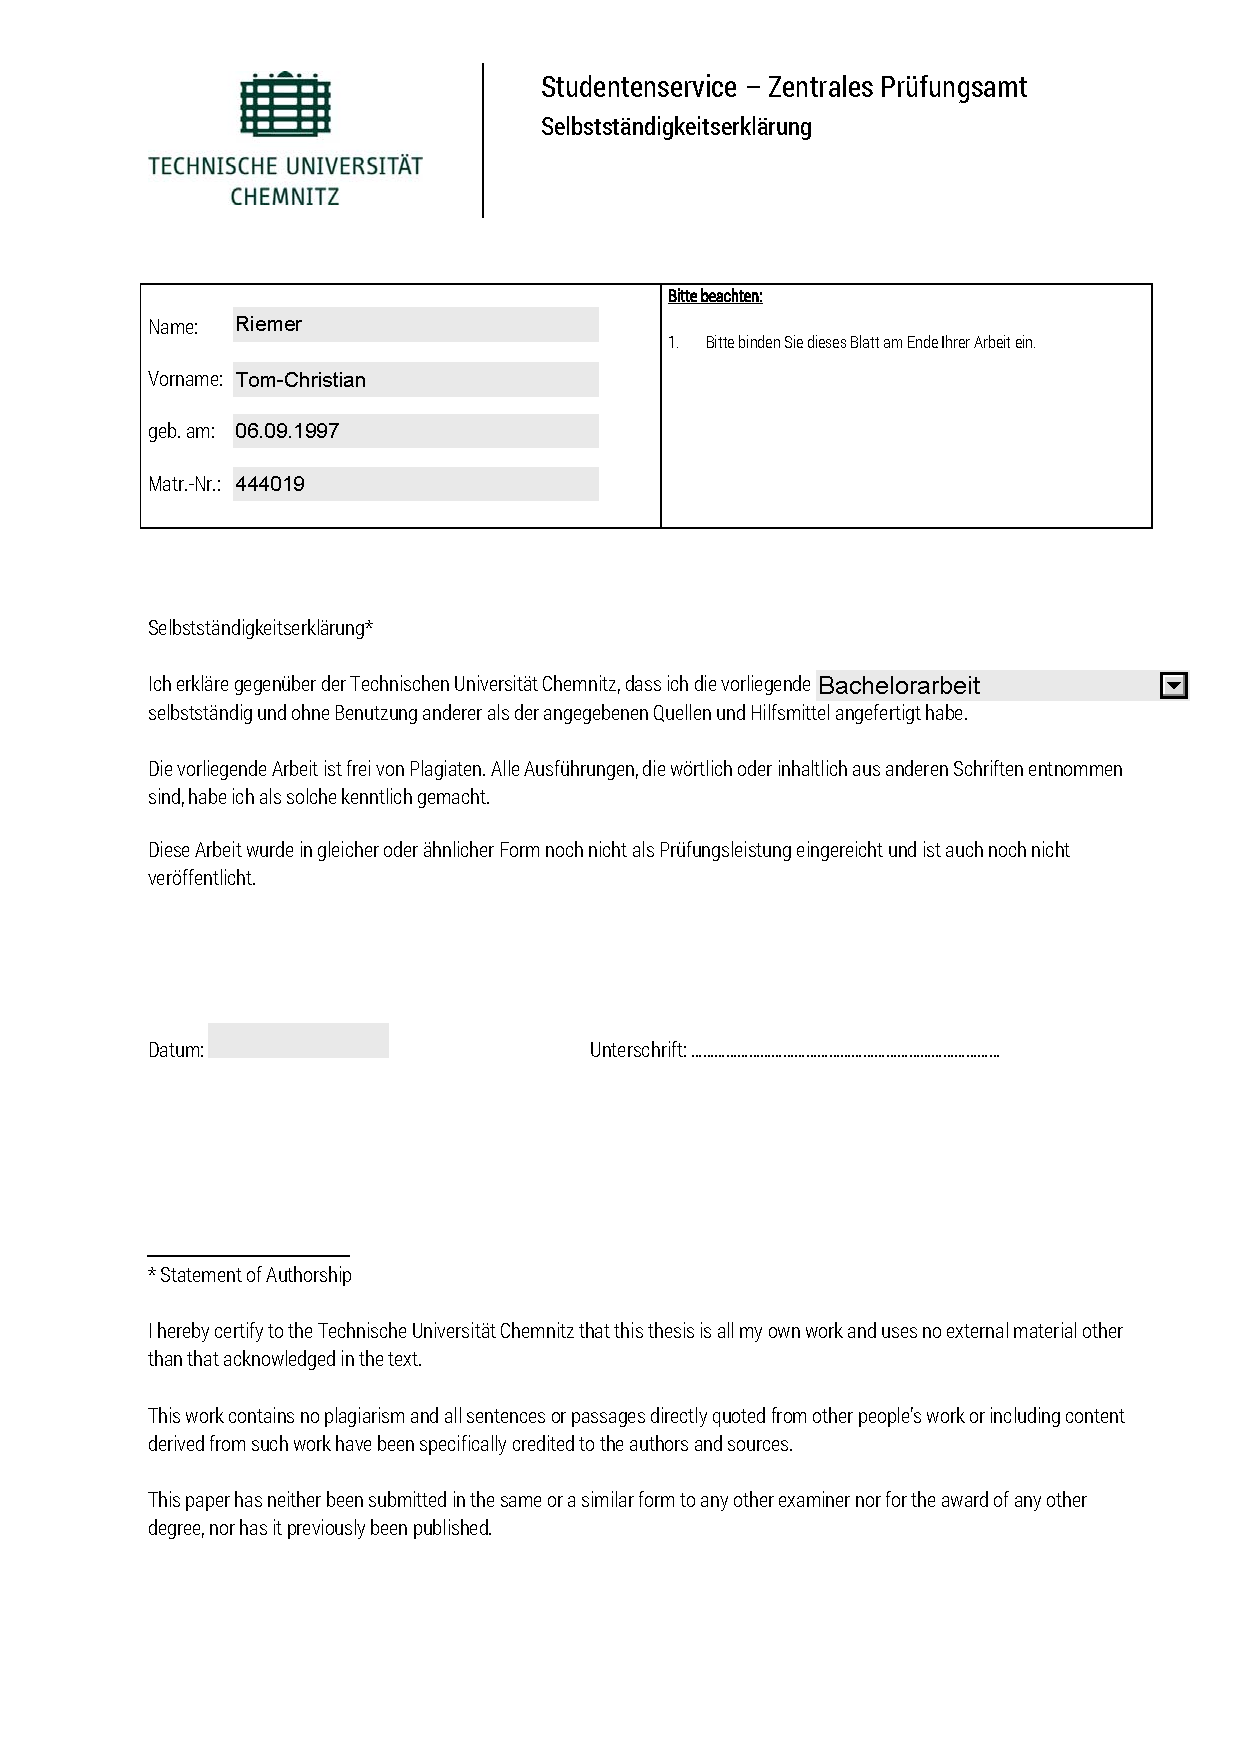
\includepdf[pages=-]{selbststaendigkeitserklaerung}
\end{document}